% Packages
% sudo tlmgr install silence appendixnumberbeamer fira fontaxes mwe noto csquotes babel helvet
%--- Preamble ---------------------------------------------------------%
% Load LaTeX packages
\documentclass[aspectratio=169]{beamer}                    % supports floating text in any location
\usetheme[darkmode]{pureminimalistic}
%\usetheme[lightmode]{pureminimalistic}

\AtBeginSection[]{%
    \frame<beamer>{
    \frametitle{Sumário para \secname}
    \setcounter{tocdepth}{10}
    \tableofcontents[currentsubsection, sectionstyle=hide/hide, subsectionstyle=show/show/hide, subsubsectionstyle=show/show/show/hide] % Show current section and current section's subsections, but hide other section's section and subsections!
  }
}
\usepackage[utf8]{inputenc}
\usepackage{csquotes,xpatch}% recommended
%\usepackage[english]{babel}
%\usepackage[american]{babel}
\usepackage[english,main=portuguese]{babel}
\usepackage{hyphenat}
\hyphenation{mate-mática recu-perar}
\usepackage{graphicx}
\usepackage{tabularx}
\usepackage{booktabs}
\usepackage{bookmark}

% Hyperlinks
\usepackage{hyperref}
\hypersetup{%
  %colorlinks=false,% hyperlinks will not be colored
  %linkbordercolor=white,
  %allcolors=white,
  %pdfborderstyle={/S/U/W 1}% border style will be underline of width 1pt
}

% Math
\usepackage{amsmath}
\usepackage{amssymb}
\usepackage{wasysym}

% Algorithms
\usepackage[ruled,vlined,portuguese]{algorithm2e}
\SetKwFor{Para}{para}{}{}

% Code
\usepackage{listings}
\usepackage{lstbayes} % Stan
\lstset{
  language=R,
  moredelim=**[is][\color{blue}]{@}{@}}

% strikethought text
\usepackage[normalem]{ulem}

% Plots
\usepackage{pgfplots}
\graphicspath{{logos}{../images}{images}}
\pgfplotsset{height=6cm, % only if needed
             width=12cm,
             compat=1.17,
             legend style = {fill = black, draw = white},
             contour/every contour label/.style={
               every node/.style={mapped color!50!black,fill=black}}
}
\usepackage{tikz}
\usepackage{tikzsymbols} % Metropolis Little Man
\usetikzlibrary{shapes}
\usetikzlibrary{arrows}
\usetikzlibrary{positioning}
\usetikzlibrary{calc}
\usetikzlibrary{automata} % State in Markov Chains
\usetikzlibrary{intersections}
\usetikzlibrary{backgrounds}
\usetikzlibrary{external}
\tikzexternalize[prefix=tikz/]
% Espaço Amostral Subfiguras
\usepackage{subfigure}
\definecolor{gray80}{gray}{0.8}
\definecolor{gray60}{gray}{0.6}
\definecolor{colorA}{rgb}{102, 255, 255}
\definecolor{colorB}{rgb}{0, 102, 255}
\usepackage{transparent}
% Modelos Multiníveis
\usepackage{adjustbox}
\newcommand*{\offset}{0.025}
\definecolor{light}{RGB}{188, 188, 220}
\definecolor{mid}{RGB}{124, 124, 185}
\definecolor{dark}{RGB}{39, 39, 143}
\definecolor{highlight}{RGB}{180, 31, 180}
% Animations
\usepackage{media9}
\usepackage{multimedia}
\addmediapath{animations}
\addmediapath{../images}

% Bibliography
\usepackage[
  backend=biber,
  doi=true,
  style=apa,
  url=true,
  eprint=false]{biblatex}
\usepackage{csquotes}
\addbibresource{../bib/bibliografia.bib}

% this makes it possible to add backup slides, without counting them
\usepackage{appendixnumberbeamer}
\renewcommand{\appendixname}{\texorpdfstring{\translate{appendix}}{appendix}}

% footer page
\renewcommand{\pageword}{Página}

% Math Font Default (Fira is strange)
\renewcommand\mathfamilydefault{\rmdefault}


% if loaded after begin{document} a warning will appear: "pdfauthor already used"
\title[Estatística Bayesiana]{Estatística Bayesiana}
\author{Jose Storopoli \newline
        \texttt{josees@uni9.pro.br}}
\institute{Universidade Nove de Julho - UNINOVE}
\date{Maio 2022}

%%%% Maths crap
\newtheorem{theo}{Theorema}[]
\newtheorem{defn}{Definição}[]
\newtheorem{question}{Questão}[]
\newtheorem{idea}{Ideia}[]
\newtheorem{exemplo}{Exemplo}[]
\newtheorem{property}{Propriedade}[]

\begin{document}
%--- Title Page -------------------------------------------------------%

\maketitle

%--- Intro Bayes for Everyone ----------------------------------------%
\begingroup
  \AtBeginSection[]{}
  \include{intro.tex}
\endgroup

%--- Table of Contents-------------------------------------------------%
\setcounter{tocdepth}{1}
\begin{frame}[plain, noframenumbering]{Sumário}
  \tableofcontents
\end{frame}

%--- Distributions ----------------------------------------------------%

\tikzset{
    declare function={
      discreteuniform(\a,\b)=1/(\b-\a+1);%
      binomial(\n,\p)=\n!/(x!*(\n-x)!)*\p^x*(1-\p)^(\n-x);%
      poisson(\l)=(\l^x)*exp(-\l)/(x!);%
      negativebinomial(\r,\p)=((x+\r-1)!/((\r-1)!*x!))*((1-\p)^x*\p^\r);%
      continuousuniform(\a,\b)=1/(\b-\a);%
      gaussian(\m,\s)=1/(\s*sqrt(2*pi))*exp(-((x-\m)^2)/(2*\s^2));%
      lognormal(\m,\s)=1/(x*\s*sqrt(2*pi))*exp(-((ln(x)-\m)^2)/(2*\s^2));%
      exponential(\l)=\l*exp(-\l*x);%
      gamma(\z)=2.506628274631*sqrt(1/\z)+ 0.20888568*(1/\z)^(1.5)+ 0.00870357*(1/\z)^(2.5)- (174.2106599*(1/\z)^(3.5))/25920- (715.6423511*(1/\z)^(4.5))/1244160)*exp((-ln(1/\z)-1)*\z;%
      student(\n)=gamma((\n+1)/2.)/(sqrt(\n*pi)*gamma(\n/2.))*((1+(x*x)/\n)^(-(\n+1)/2.));%
      beta(\a,\b)=(x^(\a-1)*(1-x)^(\b-1)/((gamma(\a)*gamma(\b))/gamma(\a+\b));%
      binormal(\ma,\sa,\mb,\sb,\ro)=exp(-(((x-\ma)/\sa)^2+((y-\mb)/\sb)^2-(2*\ro)*((x-\ma)/\sa)*((y-\mb)/\sb))/(2*(1-\ro^2)))/(2*pi*\sa*\sb*(1-\ro^2)^0.5);%
      conditionalbinormal(\yc,\ma,\sa,\mb,\sb,\ro)=exp(-(((x-\ma)/\sa)^2+((\yc-\mb)/\sb)^2-(2*\ro)*((x-\ma)/\sa)*((\yc-\mb)/\sb))/(2*(1-\ro^2)))/(2*pi*\sa*\sb*(1-\ro^2)^0.5);%
      sumtwonormals(\ma,\sa,\wa,\mb,\sb,\wb)=(\wa*gaussian(\ma,\sa))+(\wb*gaussian(\mb,\sb));%
      normcdf(\m,\s)=1/(1 + exp(-0.07056*((x-\m)/\s)^3 - 1.5976*(x-\m)/\s));%
    }
}

%--- Lectures --------------------------------------------------------%
\section{Estatística Bayesiana}

\subsection{Leituras Recomendadas}
\begin{frame}{Estatística Bayesiana - Leituras Recomendadas}
	\begin{vfilleditems}
		\item \textcite{gelman2013bayesian} - Capítulo 1: Probability and inference
		\item \textcite{mcelreath2020statistical} - Capítulo 1: The Golem of Prague
		\item \textcite{gelman2020regression} - Capítulo 3: Some basic methods in mathematics and probability
		\item \textcite{khanBayesianLearningRule2021}
		\item \textcite{storopoli2021estatisticabayesianaR} - O que é Estatística Bayesiana?
		\item \textbf{Probabilidade}:
		\begin{vfilleditems}
			\item Um ótimo livro-texto - \textcite{bertsekasIntroductionProbability2nd2008}
			\item Um ótimo livro-texto (pule a parte de estatística frequentista) - \textcite{dekkingModernIntroductionProbability2010}
			\item Do ponto de vista Bayesiano e com abordagem filosófica - \textcite{jaynesProbabilityTheoryLogic2003}
			\item Do ponto de vista Bayesiano e com abordagem simples e lúdica - \textcite{kurtBayesianStatisticsFun2019}
			\item Abordagem filosófica e uma exposição não focada no rigor matemático - \textcite{diaconisTenGreatIdeas2019}
		\end{vfilleditems}
	\end{vfilleditems}
\end{frame}

\subsection{O que é Estatística Bayesiana}
\begin{frame}{O que é Estatística Bayesiana}
	A estatística Bayesiana\footnote{maiúsculo, pois se refere ao teorema de Bayes que é um sobrenome}
	é uma abordagem de análise de dados baseada no teorema de Bayes,
	onde o conhecimento disponível sobre os parâmetros em um modelo estatístico
	é atualizado com as informações dos dados observados
	\parencite{gelman2013bayesian}. O conhecimento prévio é expresso como
	uma distribuição
	\textit{a priori}\footnote{do inglês \foreignlanguage{english}{\textit{prior distribution}}}
	e combinado com os dados observados na forma de uma função de
	verossimilhança\footnote{do inglês \foreignlanguage{english}{\textit{likelihood function}}}
	para determinar a distribuição
	posterior\footnote{\foreignlanguage{english}{do inglês \textit{posterior distribution}}}.
	A posterior também pode ser usada para fazer previsões sobre eventos futuros.
\end{frame}

\subsubsection{O que muda da Estatística Frequentista?}
\begin{frame}{O que muda da Estatística Frequentista?}
	\begin{vfilleditems}
		\item \textbf{Flexibilidade} - peças probabilísticas para construir um modelo\footnote{como se fosse LEGO}:
		\begin{vfilleditems}
			\item Conjecturas probabilísticas sobre os parâmetros:
			\begin{vfilleditems}
				\item \textit{Priori}
				\item Verossimilhança
			\end{vfilleditems}
		\end{vfilleditems}
		\item Melhor tratamento da \textbf{incerteza}:
		\begin{vfilleditems}
			\item Coerência
			\item Propagação
			\item Não se usa \textit{"se amostrássemos infinitamente de uma população que não existe..."}
		\end{vfilleditems}
		\item Sem \textbf{$p$-valores}:
		\begin{vfilleditems}
			\item Todas as intuições estatísticas fazem \textbf{sentido}
			\item 95\% de certeza que o valor do parâmetro $\theta$ está entre $x$ e $y$
			\item Quase \textbf{impossível} fazer $p$-hacking.
		\end{vfilleditems}
	\end{vfilleditems}
\end{frame}

\begin{frame}{Um pouco mais de Formalidade}
	\begin{vfilleditems}
		\item Estatística Bayesiana usa declarações probabilísticas:
		\begin{vfilleditems}
			\item um ou mais parâmetros $\theta$
			\item dados não-observados $\tilde{y}$
		\end{vfilleditems}
		\item Essas declarações são condicionadas nos valores observados de $y$:
		\begin{vfilleditems}
			\item $P(\theta \mid y)$
			\item $P(\tilde{y} \mid y)$
		\end{vfilleditems}
		\item Nós também, de maneira implícita, condicionados nos valores observados de quaisquer co-variáveis $x$
	\end{vfilleditems}
\end{frame}

\begin{frame}{Principal Mudança}
	\begin{defn}[Estatística Bayesiana]
		O uso do Teorema de Bayes\footnote{mais sobre ele já já...} como o procedimento de \textbf{estimativa dos parâmetros de interesse $\theta$ ou dados não-observados $\tilde{y}$}. \parencite{gelman2013bayesian}
	\end{defn}
\end{frame}

\subsection{Ferramentas}

\begin{frame}{Ferramentas para Estatística Bayesiana}
	\begin{vfilleditems}
		\item \LARGE  \href{https://mc-stan.org}{\texttt{Stan}}
		\item \texttt{PyMC}
		\item \small \texttt{JAGS}
		\item \footnotesize \texttt{BUGS}
	\end{vfilleditems}
\end{frame}

\subsubsection{Stan}

\begin{frame}{\href{https://mc-stan.org}{\texttt{Stan}}\footnote{\textcite{carpenterStanProbabilisticProgramming2017}}}
	\begin{columns}
		\begin{column}{0.8\textwidth}
			\begin{vfilleditems}
				\small
				\item Plataforma para modelagem e computação estatística de alto desempenho
				\item Suporte financeiro da \href{https://numfocus.org/}{NUMFocus}:
				\begin{vfilleditems}
					\footnotesize
					\item AWS Amazon
					\item Bloomberg
					\item Microsoft
					\item IBM
					\item RStudio
					\item Facebook
					\item NVIDIA
					\item Netflix
				\end{vfilleditems}
				\small
				\item Linguagem própria, similar à \texttt{C++}
				\item Amostrador \textit{Markov Chain Monte Carlo} (MCMC) em paralelo
			\end{vfilleditems}
		\end{column}
		\begin{column}{0.2\textwidth}
			\centering
			\includegraphics[width=0.6\textwidth]{stan_transparent.png}
		\end{column}
	\end{columns}
\end{frame}

\begin{frame}{\href{https://mc-stan.org}{\texttt{Stan}} na Série Billions\footnote{Se não conseguir assistir \href{https://github.com/storopoli/Estatistica-Bayesiana/blob/master/images/stan_billions_subtitled.mp4?raw=true}{clique aqui} para ver o vídeo no seu navegador} (Temporada 3 Episódio 9)}
	\centering
	\includemedia[
		width=\linewidth,
		height=0.3\linewidth,
		addresource=stan_billions_subtitled.mp4,
		transparent,
		activate=pageopen,
		passcontext,  %show VPlayer's right-click menu
		flashvars={
				source=stan_billions_subtitled.mp4
				&loop=true
				&scaleMode=stretch
			}
	]{\texttt{Stan} na Série Billions}{http://mirrors.ctan.org/macros/latex/contrib/media9/players/VPlayer.swf}
\end{frame}

% \begin{frame}[fragile]{Código \href{https://mc-stan.org}{\texttt{Stan}} versus Fórmulas de \texttt{R}}
%     \begin{lstlisting}[basicstyle=\small, language=Stan]
%     data {
%       int<lower=0> N;
%       vector[N] x1;
%       vector[N] x2;
%       vector[N] y;
%     }
%     parameters {
%       real alpha;
%       vector[2] beta;
%       real<lower=0> sigma;
%     }
%     model {
%       sigma ~ cauchy(0, 2.5);
%       y ~ normal(alpha + beta[1] * x1 + beta[2] * x2, sigma);
%     }
%     \end{lstlisting}
% \end{frame}

% \begin{frame}[fragile]{Código \href{https://mc-stan.org}{\texttt{Stan}} versus Fórmulas de \texttt{R}}
%     \begin{lstlisting}
% stan_glm(y ~ x1 + x2, data = df, family = gaussian())
%     \end{lstlisting}
% \end{frame}

% \begin{frame}{\href{https://mc-stan.org}{\texttt{Stan}}\footnote{foi lançado em 2012} na Scopus\footnote{veja as buscas Scopus nos \hyperlink{appendixscopus}{Slides de Backup no final dessa apresentação}}}
%    \centering
%    \begin{tikzpicture}[ybar]
%         \begin{axis}[
%         xlabel=Ano,ylabel=Uso,
%         x tick label style={rotate=45, /pgf/number format/.cd,
%                             scaled x ticks = false,
%                             set thousands separator={},
%                             fixed}]
%         \addplot [draw=blue, fill=blue] coordinates {
%                 (2012, 6)
%                 (2013, 19)
%                 (2014, 62)
%                 (2015, 113)
%                 (2016, 189)
%                 (2017, 387)
%                 (2018, 671)
%                 (2019, 1045)
%                 (2020, 1538)
%             };
%         \end{axis}
%     \end{tikzpicture}
% \end{frame}

% \begin{frame}{\href{https://mc-stan.org}{\texttt{Stan}}\footnote{baseado no \href{https://breckbaldwin.github.io/ScientificSoftwareImpactMetrics/DeepLearningAndBayesianSoftware.html}{reporte anual do Breck Baldwin para a NUMFocus}}\footnote{veja as buscas Scopus nos \hyperlink{appendixscopus}{Slides de Backup no final dessa apresentação}}}
%    \centering
%    \begin{tikzpicture}[ybar]
%         \begin{axis}[
%         nodes near coords={\pgfmathprintnumber[fixed,precision=3]{\pgfplotspointmeta}},
%         ylabel=Uso, xtick={1,2,3,4},
%         ymax=0.85,
%         ytick={0.1, 0.2, 0.3, 0.4, 0.5, 0.6, 0.7, 0.8},
%         xticklabels={\texttt{TensorFlow}, \texttt{PyTorch}, \texttt{Stan}, \texttt{PyMC}}]
%         \addplot [draw=yellow, fill=yellow] coordinates {
%                 (1, 0.713)};
%         \addplot [draw=green, fill=green] coordinates {
%                 (2, 0.161)};
%         \addplot [draw=blue, fill=blue] coordinates {
%                 (3, 0.108)};
%         \addplot [draw=red, fill=red] coordinates {
%                 (4, 0.0176)};
%         \end{axis}
%     \end{tikzpicture}
% \end{frame}

\subsubsection{R}
\begin{frame}{\texttt{R}}
	\begin{vfilleditems}
		\item R é uma linguagem criada \textbf{por estatísticos para estatísticos}
		\item Possui um vasto \textbf{ecossistema de bibliotecas} e é amplamente usado na \textbf{ciência} e em especial nas \textbf{ciências aplicadas}
		\item Quase toda \textbf{tese maluca} ou \textbf{algoritmo inovador} de Estatística/Probabilidade está no \texttt{CRAN} (Repositório de Pacotes \texttt{R}
		\item Como linguagem de programação é \textbf{horrível}\footnote{consegue ser um pouco menos pior que \texttt{Python}}: Recomendo \href{https://julialang.org/}{\texttt{Julia}}
	\end{vfilleditems}
\end{frame}

\subsubsection{Python}
\begin{frame}{\texttt{Python} e \href{http://docs.pymc.io/}{\texttt{PyMC}}}
	\begin{vfilleditems}
		\item \texttt{Python} consegue ser um pouco melhor que \texttt{R}
		\item Mas tem a "tara"~dos anos 90 de tudo ser \textbf{Orientado à Objetos}
		\item \href{http://docs.pymc.io/}{\texttt{PyMC}} \parencite{pymc3}:
		\begin{vfilleditems}
			\item Uma Biblioteca de Estatística Bayesiana com o seu próprio amostrador \textit{Markov Chain Monte Carlo} (MCMC)
			\item Também com Suporte financeiro da \href{https://numfocus.org/}{NUMFocus}
			\item Amarram o cavalo num barco que afundou há algum tempo: \texttt{Theano}
			\item \texttt{Theano} \textbf{morreu} mas os desenvolvedores do \texttt{PyMC} fizeram um \textit{fork} no projeto e estão usando-o como \textit{backend}
		\end{vfilleditems}
	\end{vfilleditems}
\end{frame}

% \begin{frame}[fragile]{Exemplo de Código \href{http://docs.pymc.io/}{\texttt{PyMC}}}
% \begin{lstlisting}[basicstyle=\small, language=Python]
% with Model() as model:
%     sigma = HalfCauchy("sigma", beta=10, testval=1.0)
%     alpha = Normal("Intercept", 0, sigma=20)
%     beta_1 = Normal("beta_1", 0, sigma=2)
%     beta_2 = Normal("beta_2", 0, sigma=2)

%     likelihood = Normal("y",
%                  mu=alpha + beta_1 * x1 + beta_2 * x2,
%                  sigma=sigma, observed=y)
% \end{lstlisting}
% \end{frame}

\subsubsection{Julia}
\begin{frame}{\href{https://julialang.org/}{\texttt{Julia}} e \href{https://turing.ml}{\texttt{Turing}}}
	\begin{vfilleditems}
		\item \href{https://julialang.org/}{\texttt{Julia}} \parencite{bezanson2017julia} é uma linguagem relativamente nova, lançada pela primeira vez em 2012, que visa ser de \textbf{alto nível} e \textbf{rápida}
		\item Linguagem de tipagem \textbf{dinâmica rápida} que compila \textit{just-in-time} (JIT) em código nativo usando \texttt{LLVM}.
		\item "Roda como \texttt{C}, mas lê como \texttt{Python}"~\parencite{perkelJuliaComeSyntax2019}, o que significa que é extremamente \textbf{rápida}, fácil \textbf{prototipagem} e \textbf{ler/escrever} código.
		\item \textbf{Multi-paradigma}, combinando recursos de programação \textbf{imperativa}, \textbf{funcional} e \textbf{orientada a objetos}.
	\end{vfilleditems}
\end{frame}

\begin{frame}{\href{https://turing.ml}{\texttt{Turing}}}
	\begin{vfilleditems}
		\item \href{https://turing.ml}{\texttt{Turing}} é uma \textbf{Linguagem de Programação Probabilística}\footnote{em inglês \textit{probabilistic programming language} (PPL)} escrita totalmente em \href{https://julialang.org/}{\texttt{Julia}}
		\item Usa \textbf{pacotes} de \href{https://julialang.org/}{\texttt{Julia}} para:
		\begin{vfilleditems}
			\item \textbf{Diferenciação Automática}\footnote{\textit{autodiff}}
			\item \textbf{Distribuições Probabilísticas}
			\item \textbf{Solucionadores de Equações Ordinais}\footnote{\textit{Ordinary Differential Equation Solvers} (ODE)}
			\item \textbf{Redes Neurais} (sendo responsável pela parte "Bayesiana"~da Rede Neural Bayesiana)
		\end{vfilleditems}
	\end{vfilleditems}
\end{frame}

% \begin{frame}[fragile]{Exemplo de Código \href{https://turing.ml}{\texttt{Turing}}\footnote{eu acredito que há muito potencial em \texttt{Julia} e escrevi um \href{https://storopoli.io/Bayesian-Julia}{tutorial de Estatística Bayesiana usando \texttt{Julia} e \texttt{Turing}} \parencite{storopoli2021bayesianjulia}}}
%     \begin{lstlisting}[basicstyle=\small, language=Matlab, escapeinside=\{\}]
%         @model linreg({$x_1$}, {$x_2$}, y) = begin
%             {$\alpha$} ~ Normal(0, 20)
%             {$\beta_1$} ~ Normal(0, 2)
%             {$\beta_2$} ~ Normal(0, 2)
%             {$\sigma$} ~ Exponential(1)

%             y .~ Normal({$\alpha$} .+ {$\beta_1$} * {$x_1$} + {$\beta_2$} * {$x_2$}, {$\sigma$})
%         end
%     \end{lstlisting}
% \end{frame}

\subsection{Probabilidade}
\begin{frame}{PROBABILIDADE NÃO EXISTE!\footnote{\textcite{definettiTheoryProbability1974}}}
	\begin{columns}
		\begin{column}{0.8\textwidth}
			\begin{vfilleditems}
				\item Sim, a probabilidade não existe.
				\item Ou melhor, probabilidade como uma quantidade física,
				chance objetiva, \textbf{NÃO existe}
				\item se dispensarmos a questão da chance objetiva \textit{nada se perde}
				\item A matemática do raciocínio indutivo permanece
				\textbf{exatamente a mesma}
			\end{vfilleditems}
		\end{column}
		\begin{column}{0.2\textwidth}
			\centering
			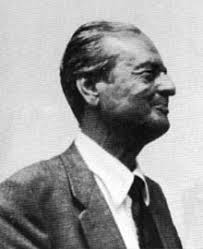
\includegraphics[width=0.9\columnwidth]{finetti.jpg}
		\end{column}
	\end{columns}
\end{frame}

\begin{frame}{PROBABILIDADE NÃO EXISTE!\footnote{\textcite{definettiTheoryProbability1974}}}
	\begin{columns}
		\begin{column}{0.6\textwidth}
			\begin{vfilleditems}
				\small
				\item Considere jogar uma moeda de enviesada
				\item As tentativas são consideradas independentes e, como resultado,
				exibem outra propriedade importante: \textbf{a ordem não importa}
				\item A frequência é considerada uma \textbf{estatística suficiente}
				\item Dizer que a ordem não importa ou dizer que a única coisa que
				importa é a frequência são duas maneiras de dizer exatamente a
				mesma coisa
				\item Dizemos que essa probabilidade é \textbf{invariante sob permutações}
			\end{vfilleditems}
		\end{column}
		\begin{column}{0.4\textwidth}
			\begin{tikzpicture}[
					scale=0.55,
					transform shape, thick,
					every node/.style = {draw, circle, minimum size = 10mm},
					grow = down,  % alignment of characters
					level 1/.style = {sibling distance=3cm},
					level 2/.style = {sibling distance=1.5cm},
					level 3/.style = {sibling distance=3cm},
					level distance = 3cm,
					head/.style = {fill = orange!90!blue,
							label = center:\textsf{\Large C}},
					tail/.style = {fill = blue!70!yellow, text = black,
							label = center:\textsf{\Large K}}
				]
				\node[shape = circle split, draw, line width = 1pt,
					minimum size = 10mm, inner sep = 0mm, font = \sffamily\large,
					rotate=30] (Start)
				{ \rotatebox{-30}{H} \nodepart{lower} \rotatebox{-30}{T}}
				child {   node [head] (A) {}
						child { node [head] (B) {}}
						child { node [tail] (C) {}}
					}
				child {   node [tail] (D) {}
						child { node [head] (E) {}}
						child { node [tail] (F) {}}
					};

				% Filling the root (Start)
				\begin{scope}[on background layer, rotate=30]
					\fill[head] (Start.base) ([xshift = 0mm]Start.east) arc (0:180:5mm)
					-- cycle;
					\fill[tail] (Start.base) ([xshift = 0pt]Start.west) arc (180:360:5mm)
					-- cycle;
				\end{scope}

				% Labels
				\begin{scope}[nodes = {draw = none}]
					\path (Start) -- (A) node [near start, left]  {$0.5$};
					\path (A)     -- (B) node [near start, left]  {$0.5$};
					\path (A)     -- (C) node [near start, right] {$0.5$};
					\path (Start) -- (D) node [near start, right] {$0.5$};
					\path (D)     -- (E) node [near start, left]  {$0.5$};
					\path (D)     -- (F) node [near start, right] {$0.5$};
					\begin{scope}[nodes = {below = 11pt}]
						\node at (B) {$0.25$};
						\node at (C) {$0.25$};
						\node at (E) {$0.25$};
						\node at (F) {$0.25$};
					\end{scope}
				\end{scope}
			\end{tikzpicture}
		\end{column}
	\end{columns}
\end{frame}

\begin{frame}{Interpretações da Probabilidade}
	\begin{vfilleditems}
		\item \textbf{Objetiva} - frequência no longo prazo de um evento específico
		\begin{vfilleditems}
			\item $P(\text{chuva}) = \frac{\text{dias que choveram}}{\text{dias totais}}$
			\item $P(\text{chance de eu ser presidente} = 0)$ (Nunca ocorreu)
		\end{vfilleditems}
		\item \textbf{Subjetiva} - nível de crença em um evento
		\begin{vfilleditems}
			\item $P(\text{chuva}) = \text{crença que choverá}$
			\item $P(\text{chance de eu ser presidente} = 10^{-10})$ (Muito improvável)
		\end{vfilleditems}
	\end{vfilleditems}
\end{frame}

\subsubsection{O que é Probabilidade?}
\begin{frame}{O que é Probabilidade?}
	\begin{defn}[Probabilidade]
		Sobre notação, definimos que $A$ é um evento e $P(A)$ a probabilidade do evento, logo:
		$$
			\{P(A) \in \mathbb{R} : 0 \leq P(A) \leq 1 \}.
		$$
		\vfill
		Isto quer dizer o "probabilidade do evento $A$ ocorrer é o conjunto de
		todos os números reais entre $0$ e $1$; incluindo $0$ e $1$"
	\end{defn}
\end{frame}

\begin{frame}{Axiomas da Probabilidade\footnote{\textcite{kolmogorovFoundationsTheoryProbability1933}}}
	\begin{columns}
		\begin{column}{0.8\textwidth}
			\begin{vfilleditems}
				\item \textbf{Não-negatividade}: Para todo $A$, $P(A) \geq 0$.
				Toda probabilidade é positiva (maior ou igual a zero), independente do
				evento
				\item \textbf{Aditividade}: Para dois \textit{mutuamente exclusivos}
				$A$ e $B$ (não podem ocorrer ao mesmo tempo):
				$P(A) = 1 - P(B)$ e $P(B) = 1 - P(A)$
				\item \textbf{Normalização}: A probabilidade de todos os eventos
				possíveis $A_1, A_2, \dots$ devem somar $1$:
				$\sum_{n \in \mathbb{N}} A_n = 1$
			\end{vfilleditems}
		\end{column}
		\begin{column}{0.2\textwidth}
			\centering
			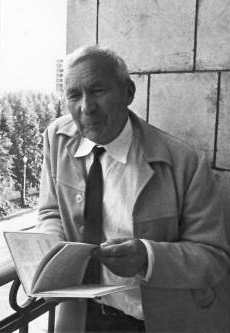
\includegraphics[width=0.9\columnwidth]{kolmogorov.jpg}
		\end{column}
	\end{columns}
\end{frame}

\begin{frame}{Espaços Amostrais}
	\begin{vfilleditems}
		\item Discretos $$\Theta = \left\{1, 2, \ldots, \right\}$$
		\item Contínuos $$\Theta \in \left(-\infty, \infty \right)$$
	\end{vfilleditems}
\end{frame}

\begin{frame}{Espaços Amostrais Discretos}
	8 Planetas do Nosso Sistema Solar
	\begin{vfilleditems}
		\item Mercúrio - $\mercury$
		\item Vênus - $\venus$
		\item Terra - $\earth$
		\item Marte $\mars$
		\item Júpiter - $\jupiter$
		\item Saturno $\saturn$
		\item Urano - $\uranus$
		\item Netuno $\neptune$
	\end{vfilleditems}
\end{frame}

\begin{frame}[fragile]{Espaços Amostrais Discretos\footnote{figuras adaptadas de \href{https://github.com/betanalpha/stan_intro}{Michael Betancourt (CC-BY-SA-4.0)}}}
	\footnotesize
	\begin{figure}
		\centering
		\subfigure{
			\begin{tikzpicture}[scale=0.25, thick]
				\draw[color=black] (-25, 0) to (10, 0);
				\node[] at (-15, 0) {O planeta possui campo magnético};
				\node[] at (7, 2) {$\theta \in E_{1}$};

				\fill[color=gray60] (0, 0) circle (25pt) node[color=black] {$\mercury$};
				\fill[color=blue] (2, 0) circle (25pt) node[color=black] {$\venus$};
				\fill[color=blue] (4, 0) circle (25pt) node[color=black] {$\earth$};
				\fill[color=gray60] (6, 0) circle (25pt) node[color=black] {$\mars$};
				\fill[color=blue] (8, 0) circle (25pt) node[color=black] {$\jupiter$};
				\fill[color=blue] (10, 0) circle (25pt) node[color=black] {$\saturn$};
				\fill[color=blue] (12, 0) circle (25pt) node[color=black] {$\uranus$};
				\fill[color=blue] (14, 0) circle (25pt) node[color=black] {$\neptune$};
			\end{tikzpicture}
		}
		%
		\subfigure{
			\begin{tikzpicture}[scale=0.25, thick]
				\draw[color=black] (-25, 0) to (10, 0);
				\node[] at (-15, 0) {O planeta possui luas};
				\node[] at (7, 2) {$\theta \in E_{2}$};

				\fill[color=gray60] (0, 0) circle (25pt) node[color=black] {$\mercury$};
				\fill[color=gray60] (2, 0) circle (25pt) node[color=black] {$\venus$};
				\fill[color=blue] (4, 0) circle (25pt) node[color=black] {$\earth$};
				\fill[color=blue] (6, 0) circle (25pt) node[color=black] {$\mars$};
				\fill[color=blue] (8, 0) circle (25pt) node[color=black] {$\jupiter$};
				\fill[color=blue] (10, 0) circle (25pt) node[color=black] {$\saturn$};
				\fill[color=blue] (12, 0) circle (25pt) node[color=black] {$\uranus$};
				\fill[color=blue] (14, 0) circle (25pt) node[color=black] {$\neptune$};
			\end{tikzpicture}
		}
		%
		\subfigure{
			\begin{tikzpicture}[scale=0.25, thick]
				\draw[color=black] (-25, 0) to (10, 0);
				\node[] at (-15, 0) {O planeta possui campo magnético e luas};
				\node[] at (7, 2) {$\theta \in E_{1} \cap E_{2}$};

				\fill[color=gray60] (0, 0) circle (25pt) node[color=black] {$\mercury$};
				\fill[color=gray60] (2, 0) circle (25pt) node[color=black] {$\venus$};
				\fill[color=blue] (4, 0) circle (25pt) node[color=black] {$\earth$};
				\fill[color=gray60] (6, 0) circle (25pt) node[color=black] {$\mars$};
				\fill[color=blue] (8, 0) circle (25pt) node[color=black] {$\jupiter$};
				\fill[color=blue] (10, 0) circle (25pt) node[color=black] {$\saturn$};
				\fill[color=blue] (12, 0) circle (25pt) node[color=black] {$\uranus$};
				\fill[color=blue] (14, 0) circle (25pt) node[color=black] {$\neptune$};
			\end{tikzpicture}
		}
		%
		\subfigure{
			\begin{tikzpicture}[scale=0.25, thick]
				\node[] at (-15, 0) {O planeta possui campo magnético ou luas};
				\node[] at (7, 2) {$\theta \in E_{1} \cup E_{2}$};

				\fill[color=gray60] (0, 0) circle (25pt) node[color=black] {$\mercury$};
				\fill[color=blue] (2, 0) circle (25pt) node[color=black] {$\venus$};
				\fill[color=blue] (4, 0) circle (25pt) node[color=black] {$\earth$};
				\fill[color=blue] (6, 0) circle (25pt) node[color=black] {$\mars$};
				\fill[color=blue] (8, 0) circle (25pt) node[color=black] {$\jupiter$};
				\fill[color=blue] (10, 0) circle (25pt) node[color=black] {$\saturn$};
				\fill[color=blue] (12, 0) circle (25pt) node[color=black] {$\uranus$};
				\fill[color=blue] (14, 0) circle (25pt) node[color=black] {$\neptune$};
			\end{tikzpicture}
		}
		%
		\subfigure{
			\begin{tikzpicture}[scale=0.25, thick]
				\node[] at (-15, 0) {O planeta não possui um campo magnético};
				\node[] at (7, 2) {$\theta \in \neg E_{1}$};

				\fill[color=blue] (0, 0) circle (25pt) node[color=black] {$\mercury$};
				\fill[color=gray60] (2, 0) circle (25pt) node[color=black] {$\venus$};
				\fill[color=gray60] (4, 0) circle (25pt) node[color=black] {$\earth$};
				\fill[color=blue] (6, 0) circle (25pt) node[color=black] {$\mars$};
				\fill[color=gray60] (8, 0) circle (25pt) node[color=black] {$\jupiter$};
				\fill[color=gray60] (10, 0) circle (25pt) node[color=black] {$\saturn$};
				\fill[color=gray60] (12, 0) circle (25pt) node[color=black] {$\uranus$};
				\fill[color=gray60] (14, 0) circle (25pt) node[color=black] {$\neptune$};
			\end{tikzpicture}
		}
		%
	\end{figure}
\end{frame}

\begin{frame}{Espaços Amostrais Contínuos\footnote{figuras adaptadas de \href{https://github.com/betanalpha/stan_intro}{Michael Betancourt (CC-BY-SA-4.0)}}}
	\footnotesize
	\begin{figure}
		\centering
		\subfigure{
			\begin{tikzpicture}[scale=0.25, thick]
				\draw[color=black] (-27, 0) to (17, 0);
				\node[align=center] at (-15, 0) {A distância é menos que cinco centímetros};
				\node[] at (7.5, 2) {$\theta \in E_{1}$};

				\draw[|->] (0, 0) -- (14,0) node[right] {$x$};
				\draw[line width=1mm, color=blue] (0, 0) node[] {$\,($} -- (5, 0) node[] {$\!)$};
			\end{tikzpicture}
		}
		%
		\subfigure{
			\begin{tikzpicture}[scale=0.25, thick]
				\draw[color=black] (-27, 0) to (17, 0);
				\node[align=center] at (-15, 0) {A distância é entre três e sete centímetros};
				\node[] at (7.5, 2) {$\theta \in E_{2}$};

				\draw[|->] (0, 0) -- (14,0) node[right] {$x$};
				\draw[line width=1mm, color=blue] (3, 0) node[] {$\,($} -- (7,0) node[] {$\!)$};

			\end{tikzpicture}
		}
		%
		\subfigure{
			\begin{tikzpicture}[scale=0.25, thick]
				\draw[color=black] (-27, 0) to (17, 0);
				\node[align=center] at (-15, 0) {A distância é menos que cinco centímetros \\ e entre três e sete centímetros};
				\node[] at (7.5, 2) {$\theta \in E_{1} \cap E_{2}$};

				\draw[|->] (0, 0) -- (14,0) node[right] {$x$};
				\draw[line width=1mm, color=blue] (3, 0) node[] {$\,($} -- (5, 0) node[] {$\!)$};
			\end{tikzpicture}
		}
		%
		\subfigure{
			\begin{tikzpicture}[scale=0.25, thick]
				\draw[color=black] (-27, 0) to (17, 0);
				\node[align=center] at (-15, 0) {A distância é menos que cinco centímetros \\ ou entre três e sete centímetros};
				\node[] at (7.5, 2) {$\theta \in E_{1} \cup E_{2}$};

				\draw[|->] (0, 0) -- (14, 0) node[right] {$x$};
				\draw[line width=1mm, color=blue] (0, 0) node[] {$\,($} -- (7, 0) node[] {$\!)$};
			\end{tikzpicture}
		}
		%
		\subfigure{
			\begin{tikzpicture}[scale=0.25, thick]
				\draw[color=black] (-27, 0) to (17, 0);
				\node[align=center] at (-15, 0) {A distância não é menos que cinco centímetros};
				\node[] at (7.5, 2) {$\theta \in \neg E_{1}$};

				\draw[|->] (0, 0) -- (14, 0) node[right] {$x$};
				\draw[line width=1mm, color=blue] (5, 0) node[] {$\,($} -- (13, 0);
			\end{tikzpicture}
		}
	\end{figure}
\end{frame}

\begin{frame}{Parâmetros Discretos versus Contínuos}

	Tudo o que foi exposto até agora partiu do pressuposto que os parâmetros
	são discretos. Isto foi feito com o intuito de prover uma melhor intuição
	do que é probabilidade. Nem sempre trabalhamos com parâmetros discretos.
	Os parâmetros podem ser contínuos, como por exemplo: idade, altura, peso etc.
	Mas não se desespere, todas as regras e axiomas da probabilidade são válidos
	também para parâmetros contínuos. A única coisa que temos que fazer é trocar
	todas as somas $\sum$ por integrais $\int$. Por exemplo o terceiro axioma de
	\textbf{Normalização} para variáveis aleatórias contínuas se torna:

	$$
		\int_{x \in X} p(x) dx = 1.
	$$

\end{frame}


\begin{frame}{Probabilidade Condicional}
	\begin{defn}[Probabilidade Condicional]
		Probabilidade de um evento ocorrer caso outro tenha ocorrido ou não. \newline \newline
		A notação que usamos é $P( A \mid B )$, que lê-se como "a probabilidade
		de observamos $A$ dado que já observamos $B$". \newline \newline
		\vfill \vfill
		$$
			\begin{aligned}
				P(A \mid B) & = \frac{\text{número de elementos em $A$ e $B$}}{\text{número de elemementos em $B$}} \\
				P(A \mid B) & = \frac{P(A \cap B)}{(B)}
			\end{aligned}
		$$
		\newline \newline \hspace{0.7\textwidth}
		{\footnotesize assumimos que $P(B) > 0$}.
	\end{defn}
\end{frame}

\begin{frame}{Exemplo de Probabilidade Condicional}
	\begin{exemplo}[Poker Texas Hold'em]
		\begin{vfilleditems}
			\item \textbf{Espaço Amostral}: $52$ cartas no baralho, $13$ tipos de cartas e $4$ tipos de naipes.
			\item $P(A)$: Chance de receber um Ás $\left( \frac{4}{52} = \frac{1}{13}\right)$
			\item $P(K)$: Chance de receber um Rei (K) $\left( \frac{4}{52} = \frac{1}{13} \right)$
			\item $P(A \mid K)$: Chance de receber um Ás, dado que você recebeu um Rei (K) $\left( \frac{4}{51} \approx 0.078 \right)$
			\item $P(K \mid A)$: Chance de receber um Rei (K), dado que você recebeu um Ás $\left( \frac{4}{51} \approx 0.078 \right)$
		\end{vfilleditems}
	\end{exemplo}
\end{frame}

\begin{frame}{Cuidado! Nem sempre $P(A \mid B) = P(B \mid A)$}
	No exemplo anterior temos a simetria $P(A \mid K) = P(K \mid A)$, \textbf{mas nem sempre isso é verdade}\footnote{Mais especificamente, se as taxas basais $P(A)$ e $P(B)$ não são iguais, a simetria é quebrada $P(A \mid B) \neq P(B \mid A)$!}
	\begin{exemplo}[O Papa é católico]
		\begin{vfilleditems}
			\small{
				\item $P(\text{papa})$: Chance alguém aleatório ser papa, algo bem pequeno, 1 em 8 bilhões $\left( \frac{1}{8 \cdot 10^9} \right)$
				\item $P(\text{católico})$: Chance alguém aleatório ser católico, 1.34 de 8 bilhões $\left( \frac{1.34}{8} \approx 0.17 \right)$
				\item $P(\text{católico} \mid \text{papa})$: Chance do Papa ser católico $\left( \frac{999}{1000} = 0.999 \right)$
				\item $P(\text{papa} \mid \text{católico})$: Chance de alguém católico ser o papa $\left( \frac{1}{1.34 \cdot 10^9} \cdot 0.999 \approx 7.46 \cdot 10^{-10} \right)$
			}
			\item \large{\textbf{Logo}: $P(\text{católico} \mid \text{papa}) \neq P(\text{papa} \mid \text{católico})$}
		\end{vfilleditems}
	\end{exemplo}
\end{frame}

\begin{frame}{Um clássico da Probabilidade}
	\begin{columns}
		\begin{column}{0.6\textwidth}
			\begin{exemplo}[Monty Hall]
				\begin{vfilleditems}
					\small
					\item Um apresentador de TV lhe apresenta 3 portas
					\item Uma delas tem um prêmio: um carro! As outras tem um bode
					\item Você deve escolher uma porta (que não é aberta)
					\item Nesse momento Monty abre uma das outras duas portas que você
					não escolheu, revelando que o carro não se encontra nessa porta e revelando um dos bodes
					\item Monty então lhe pergunta "Você quer manter sua escolha de porta ou trocar?"
				\end{vfilleditems}
			\end{exemplo}
		\end{column}
		\begin{column}{0.4\textwidth}
			\begin{figure}
				\centering
				\def\svgwidth{\columnwidth}
				\input{../images/monty_hall.pdf_tex}
			\end{figure}
		\end{column}
	\end{columns}
\end{frame}

\begin{frame}{Solução do Problema de Monty Hall}
	\begin{idea}[Probabilidade de ganhar o carro]
		$$
			\begin{aligned}
				P(\text{carro} \mid C_i) & = \frac{1}{3}                                                                                                                          \\
				P(\text{carro})          & = \frac{1}{3} \cdot P(\text{carro} \mid C_1) + \frac{1}{3} \cdot P(\text{carro} \mid C_2) + \frac{1}{3} \cdot P(\text{carro} \mid C_3) \\
				P(\text{carro})          & = \frac{\sum^3_{i=1}P(\text{carro} \mid C_i)}{3}                                                                                       \\
				P(\text{carro})          & = \frac{1}{3}
			\end{aligned}
		$$
	\end{idea}
	\vfill \vfill
	$C_i$ é o evento no qual o carro está atrás da porta $i$, $i=1,2,3$
\end{frame}

\begin{frame}[t]{Solução do Problema de Monty Hall\footnote{se você não acredita nesse resultado veja como simular o problema de Monty Hall nos \hyperlink{appendixmontyhall}{Slides de Backup no final dessa apresentação}}}
	\begin{columns}[t]
		\begin{column}{0.5\textwidth}
			{\Large \textbf{Cenário 1}: Não trocar de porta} \newline \newline
			Simples: $$\frac{1}{3}$$
		\end{column}
		\begin{column}{0.5\textwidth}
			{\Large \textbf{Cenário 2}: Trocar de porta} \newline \newline
			Escolha qualquer porta $i$ para ser $C_i = 0$
			\vfill
			$$
				\begin{aligned}
					P(\text{carro}) & = 0 \cdot P(\text{carro} \mid C_i) + \frac{1}{3} + \frac{1}{3} \\
					P(\text{carro}) & = \frac{2}{3}
				\end{aligned}
			$$
		\end{column}
	\end{columns}
\end{frame}

\begin{frame}{Visualização do Problema de Monty Hall}
	\begin{figure}
		\centering
		\subfigure{
			\begin{tikzpicture}[
					scale=0.55,
					header/.style = {draw, rectangle, fill = blue!50!black, minimum size = 10mm},
					level distance = 3.5cm,
					transform shape, thick,
					grow = right, sloped,
				]
				\node[header] {Sua Escolha}
				child{
						node[header] {Carro está}
						edge from parent[draw=none]
						child{
								node[header] {Monty abre}
								edge from parent[draw=none]
								child{
										node[header] {resultado}
										edge from parent[draw=none]
									}
							}
					};
			\end{tikzpicture}
		}
		%
		\subfigure{
			\begin{tikzpicture}[
					scale=0.55,
					door/.style = {draw, circle, minimum size = 10mm},
					car/.style = {circle, fill = green!50!black, minimum size = 10mm},
					goat/.style = {circle, fill = red!50!black, minimum size = 10mm},
					level distance = 3.5cm,
					transform shape, thick,
					grow = right, sloped,
					level 1/.style = {sibling distance=3.5cm},
					level 2/.style = {sibling distance=2cm},
					level 3/.style = {sibling distance=3cm}
				]
				\node[door] {Porta 1}
				child {
				node[door] {Porta 3}
				child {
				node[door] {Porta 2}
				child {
				node[car, label=right:{\Large$\frac{1}{3}$}] {Carro}
				}
				edge from parent
				node[above] {\Large$1$}
				}
				edge from parent
				node[below] {\Large$\frac{1}{3}$}
				}
				child {
				node[door] {Porta 2}
				child {
				node[door] {Porta 3}
				child {
				node[car, label=right:{\Large$\frac{1}{3}$}] {Carro}
				}
				edge from parent
				node[above] {\Large$1$}
				}
				edge from parent
				node[above] {\Large$\frac{1}{3}$}
				}
				child {
				node[door] {Porta 1}
				child {
				node[door] {Porta 2}
				child {
				node[goat, label=right:{\Large$\frac{1}{6}$}] {Bode}
				}
				edge from parent
				node[above]  {\Large$\frac{1}{2}$}
				}
				child {
				node[door] {Porta 3}
				child {
				node[goat, label=right:{\Large$\frac{1}{6}$}] {Bode}
				}
				edge from parent
				node[above]  {\Large$\frac{1}{2}$}
				}
				edge from parent
				node[above] {\Large$\frac{1}{3}$}
				};
			\end{tikzpicture}
		}
	\end{figure}
\end{frame}

\begin{frame}{Probabilidade Conjunta}
	\begin{defn}[Probabilidade Conjunta]
		Probabilidade de observados dois ou mais eventos ocorrem. \newline \newline
		A notação que usamos é $P(A, B)$, que lê-se como
		"a probabilidade de observamos $A$ e também observamos $B$". \newline \newline
		$$
			\begin{aligned}
				P(A,B) & = \text{número de elementos em $A$ ou $B$} \\
				P(A,B) & = P(A \cup B)
			\end{aligned}
		$$
	\end{defn}
\end{frame}

\begin{frame}{Exemplo de Probabilidade Conjunta}
	\begin{exemplo}[Revisitando Poker Texas Hold'em]
		\begin{vfilleditems}
			{\footnotesize
				\item \textbf{Espaço Amostral}: $52$ cartas no baralho, $13$ tipos de cartas e $4$ tipos de naipes.
				\item $P(A)$: Chance de receber um Ás $\left( \frac{4}{52} = \frac{1}{13}\right)$
				\item $P(K)$: Chance de receber um Rei (K) $\left( \frac{4}{52} = \frac{1}{13} \right)$
				\item $P(A \mid K)$: Chance de receber um Ás, dado que você recebeu um Rei (K) $\left( \frac{4}{51} \approx 0.078 \right)$
				\item $P(K \mid A)$: Chance de receber um Rei (K), dado que você recebeu um Ás $\left( \frac{4}{51} \approx 0.078 \right)$
			}
			\item $P(A, K)$: Chance de receber um Ás e um Rei (K)
			$$
				\begin{aligned}
					P(A, K)                         & = P(K, A)                         \\
					P(A) \cdot P(K \mid A)          & = P(K) \cdot P(A \mid K)          \\
					\frac{1}{13} \cdot \frac{4}{51} & = \frac{1}{13} \cdot \frac{4}{51} \\
					                                & \approx 0.006
				\end{aligned}
			$$
		\end{vfilleditems}
	\end{exemplo}
\end{frame}

% Exemplo do Poker com pacote pst-poker
% Exemplo do Papa e Católico

% Bivariate Normal inspirada aqui: https://github.com/walmes/Tikz/blob/master/src/bivariate-normal.pgf
\begin{frame}{Visualização de Probabilidade Conjunta vs Probabilidade Condicional}
	\centering
	\begin{tikzpicture}[scale=0.9]
		\begin{axis}[
				domain   = -3.5:3.5,
				domain y = -3.5:3.5,
				view = {-70}{20},
				title={$P(X,Y)$ versus $P(X \mid Y=-0.75)$},
				xlabel={$X$},
				ylabel={$Y$},
				% zlabel={$SSE(\beta_0, \beta_1)$},
				zmin = -0,
				%xticklabels=\empty,
				%yticklabels=\empty,
				zticklabels=\empty,
				xtick=\empty,
				ytick={-0.75},
				ztick=\empty,
				axis z line*=none,
				axis y line*=left,
				axis x line*= bottom]
			\addplot3 [
				domain = -3.5:3.5,
				samples = 50, samples y = 0,
				thick, smooth, color = red, fill = orange, opacity = 0.75]
			(x, -0.75, {conditionalbinormal(-0.75, 0, 1, 0, 1, 0.75)});

			\draw (-3.5, -0.75, 0) -- (3.5, -0.75, 0);

			\addplot3 [
				surf,
				domain = -3.5:3.5,
				samples = 50,
				opacity = 0.15,
				faceted color = colorB,
				colormap = {blueblack}{
						color = (colorB)
						color = (colorA!50!white)
						color = (colorA)}]
			{binormal(0, 1, 0, 1, 0.7)};
		\end{axis}
	\end{tikzpicture}
\end{frame}

% Countour plot inspirado daqui: https://tex.stackexchange.com/a/31713/200209
\begin{frame}{Visualização de Probabilidade Conjunta vs Probabilidade Condicional}
	\begin{columns}
		\begin{column}{0.5\textwidth}
			\centering
			\begin{tikzpicture}[scale=0.5]
				\begin{axis}[
						view={0}{90},
						axis equal,
						enlarge y limits=true,
						title={$P(X,Y)$},
						xlabel={$X$},
						ylabel={$Y$},
						xtick=\empty,
						ytick={-0.75}
					]

					\draw[red, line width=2pt] (-3.5, -0.75) -- (3.5, -0.75);

					\addplot3[contour gnuplot={labels=false},domain=-3.5:3.5,domain y=-3.5:3.5]
					{exp(-( x^2 + y^2)/3 )};

				\end{axis}
			\end{tikzpicture}
		\end{column}
		\begin{column}{0.5\textwidth}
			\centering
			\begin{tikzpicture}[scale=0.5]
				\begin{axis}[every axis plot, line width=2pt,
						title={$P(X \mid Y=-0.75)$},
						xlabel={$X$},
						ylabel={$Y$},
						xtick=\empty,
						ytick=\empty,
						domain=-3.5:3.5,samples=200,
						axis x line*=bottom, % no box around the plot, only x and y axis
						axis y line*=left, % the * suppresses the arrow tips
						enlarge x limits=true
					] % extend the axes a bit

					\addplot [red, fill = red, fill opacity = 0.5] {exp(-( x^2 + -0.75^2)/3 )};
				\end{axis}
			\end{tikzpicture}
		\end{column}
	\end{columns}
\end{frame}

\subsubsection{Teorema de Bayes}
\begin{frame}{Quem foi Thomas Bayes?}
	\begin{columns}
		\begin{column}{0.8\textwidth}
			\begin{vfilleditems}
				\item \small Thomas Bayes (1701 - 1761) foi um estatístico, filósofo
				e ministro presbiteriano inglês conhecido por formular um caso
				específico do teorema que leva seu nome
				\item \small Bayes nunca publicou o que se tornaria sua realização mais famosa;
				suas notas foram editadas e publicadas após sua morte pelo seu amigo
				Richard Price
				\item \small O nome formal do teorema é Bayes-Price-Laplace, pois Thomas
				Bayes foi o primeiro a descobrir, Richard Price pegou seus rascunhos,
				formalizou em notação matemática e apresentou para a Royal Society of London,
				e Pierre Laplace redescobriu o teorema sem ter tido contato prévio no final
				do século XVIII na França ao usar probabilidade para inferência estatística
				com dados do Censo na era Napoleônica
			\end{vfilleditems}
		\end{column}
		\begin{column}{0.2\textwidth}
			\centering
			\includegraphics[width=0.9\columnwidth]{thomas_bayes.png}
		\end{column}
	\end{columns}
\end{frame}


\begin{frame}{Teorema de Bayes}
	\begin{theo}[Bayes]
		Nos diz como "inverter" a probabilidade condicional: \newline \newline
		$$P(A \mid B) = \frac{P(A) \cdot P(B \mid A)}{P(B)}$$
	\end{theo}
\end{frame}

\begin{frame}{Prova do Teorema de Bayes}
	Lembra que temos a seguinte identidade na probabilidade:
	$$
		\begin{aligned}
			P(A,B)                 & = P(B,A)                 \\
			P(A) \cdot P(B \mid A) & = P(B) \cdot P(A \mid B)
		\end{aligned}
	$$

	Pois bem, agora passe o $P(B)$ do lado direito para o lado esquerdo dividindo:
	$$
		\begin{aligned}
			P(A) \cdot P(B \mid A)              & = \overbrace{P(B)}^{\text{isso vai para $\leftarrow$}} \cdot \quad P(A \mid B) \\
			                                    &                                                                                \\
			\frac{P(A) \cdot P(B \mid A)}{P(B)} & = P(A \mid B)                                                                  \\
			P(A \mid B)                         & = \frac{P(A) \cdot P(B \mid A)}{P(B)}
		\end{aligned}
	$$
\end{frame}

\begin{frame}{Visualização do Teorema de Bayes}
	\begin{columns}
		\begin{column}{0.6\textwidth}
			\begin{tikzpicture}[thick]
				\node[circle, label={137:Espaço Amostral}, fill=red!20!white, fill opacity = 0.5, minimum size=6cm] (Omega) at (0,0) {};
				\node[ellipse, label={35:$E_1$}, fill=blue, fill opacity = 0.5, minimum width=5.5cm, minimum height=2cm] (Ellipse) at (0,1) {};
				\node[circle, label={178:$E_2$}, fill=red, fill opacity = 0.5, minimum size = 1cm] (Circulo) at (-1.5,1) {};
				\node[] (KK) at (-1.5, 1) {$KK$};
				\node[] (CC) at (1.5, 1) {$CC$};
				\node[] (KC) at (1.5, -1) {$KC$};
				\node[] (CK) at (-1.5, -1) {$CK$};
			\end{tikzpicture}
		\end{column}
		\begin{column}{0.4\textwidth}
			$$
				\begin{aligned}
					E_1 & = P(KK  \cup CC) \\
					E_2 & = P(KK \mid E_1)
				\end{aligned}
			$$
		\end{column}
	\end{columns}
\end{frame}

\begin{frame}{Mais um clássico da Probabilidade\footnote{Origem: \href{https://www.yudkowsky.net/rational/bayes}{Yudkowski - \textit{An Intuitive Explanation of Bayes’ Theorem}}}}
	\begin{exemplo}[Cancêr de Mama]
		\small
		O quão acurado é o teste de \textbf{câncer de mama}?
		\begin{vfilleditems}
			\item \footnotesize 1\% das mulheres têm \textbf{câncer de mama} (Prevalência)
			\item \footnotesize 80\% das mamografias detectam o \textbf{câncer de mama} (Verdadeiro Positivo)
			\item \footnotesize 9.6\% das mamografias detectam \textbf{câncer de mama} quando não há incidência (Falso Positivo)
		\end{vfilleditems}
		$$
			\begin{aligned}
				P(C \mid +) & = \frac{P(+ \mid C) \cdot P(C)}{P(+)}                                                      \\
				P(C \mid +) & = \frac{P(+ \mid C) \cdot P(C)}{P(+ \mid C) \cdot P(C) + P(+ \mid \neg C) \cdot P(\neg C)} \\
				P(C \mid +) & = \frac{0.8 \cdot 0.01}{0.8 \cdot 0.01 + 0.096 \cdot 0.99}                                 \\
				P(C \mid +) & \approx 0.0776
			\end{aligned}
		$$
	\end{exemplo}
\end{frame}


\begin{frame}{Porquê o teorema de Bayes é Importante?}
	\begin{idea}[Podemos Inverter a Probabilidade Condicional]
		$$
			\begin{aligned}
				P(\text{hipótese} \mid \text{dados}) = \frac{P(\text{hipótese}) \cdot P(\text{dados} \mid \text{hipótese})}{P(\text{data})}
			\end{aligned}
		$$
	\end{idea}
	Mas isso não é o $p$-valor? \textcolor{red}{\textbf{NÃO!}}
\end{frame}

\subsection{Estatística Frequentista versus Bayesiana}
\subsubsection{O que são $p$-valores e Intervalos de Confiança}
\begin{frame}{O que é o $p$-valor?}
	\begin{defn}[$p$-valor]
		$p$-valor é a probabilidade de obter resultados no mínimo tão
		extremos quanto os que foram observados, dado que a hipótese nula
		$H_0$ é verdadeira
		$$P(D \mid H_0)$$
	\end{defn}
\end{frame}

\begin{frame}{O que \textbf{não é} o $p$-valor!}
	\centering
	\includegraphics[width=0.7\textwidth]{meme-pvalue.jpg}
\end{frame}

\begin{frame}{O que \textbf{não é} o $p$-valor!}
	\begin{vfilleditems}
		\item \textbf{$p$-valor não é a probabilidade da Hipótese nula}
		- Famosa confusão entre $P(D \mid H_0)$ e $P(H_0 \mid D)$.
		Para obter a $P(H_0 \mid D)$ você precisa de estatística Bayesiana.
		\item \textbf{$p$-valor não é a probabilidade dos dados serem produzidos pelo acaso}
		- \textcolor{red}{Não!} Ninguém falou nada de acaso.
		\item \textbf{$p$-valor mensura o tamanho do efeito de um teste estatístico}
		- Também \textcolor{red}{não}... $p$-valor não diz nada sobre o tamanho do efeito.
		Apenas sobre se o quanto os dados observados divergem do esperado sob a hipótese nula.
		Além disso, $p$-valores podem ser "hackeados" de diversas maneiras \parencite{head2015extent}.
	\end{vfilleditems}
\end{frame}

\begin{frame}{A relação entre $p$-valor e $H_0$}
	Para descobrir o $p$-valor, \textbf{descubra a $H_0$ que está por trás dele}.
	Sua definição nunca mudará, pois ela sempre é $P(D \mid H_0)$:
	\begin{vfilleditems}
		\item \textbf{Teste $t$}: $P(D \mid \text{a diferença entre os grupos é zero})$
		\item \textbf{ANOVA}: $P(D \mid \text{não há diferença entre os grupos})$
		\item \textbf{Regressão}: $P(D \mid \text{coeficiente é nulo})$
		\item \textbf{Shapiro-Wilk}: $P(D \mid \text{população é distribuída como uma normal})$
	\end{vfilleditems}
\end{frame}

\begin{frame}{O que são Intervalos de Confiança?}
	\begin{columns}
		\begin{column}{0.8\textwidth}
			\begin{defn}[Intervalos de Confiança]
				\begin{quotation}
					Um intervalo de confiança de X\% para um parâmetro é um intervalo
					$(a, b)$ gerado por um procedimento que em amostragem repetida
					tem uma probabilidade de X\% de conter o valor verdadeiro do
					parâmetro, para todos os valores possíveis do parâmetro
				\end{quotation}
				\vfill \vfill
				\textcite{neyman1937outline} (o "pai" dos intervalos de confiança)
			\end{defn}
		\end{column}
		\begin{column}{0.2\textwidth}
			\centering
			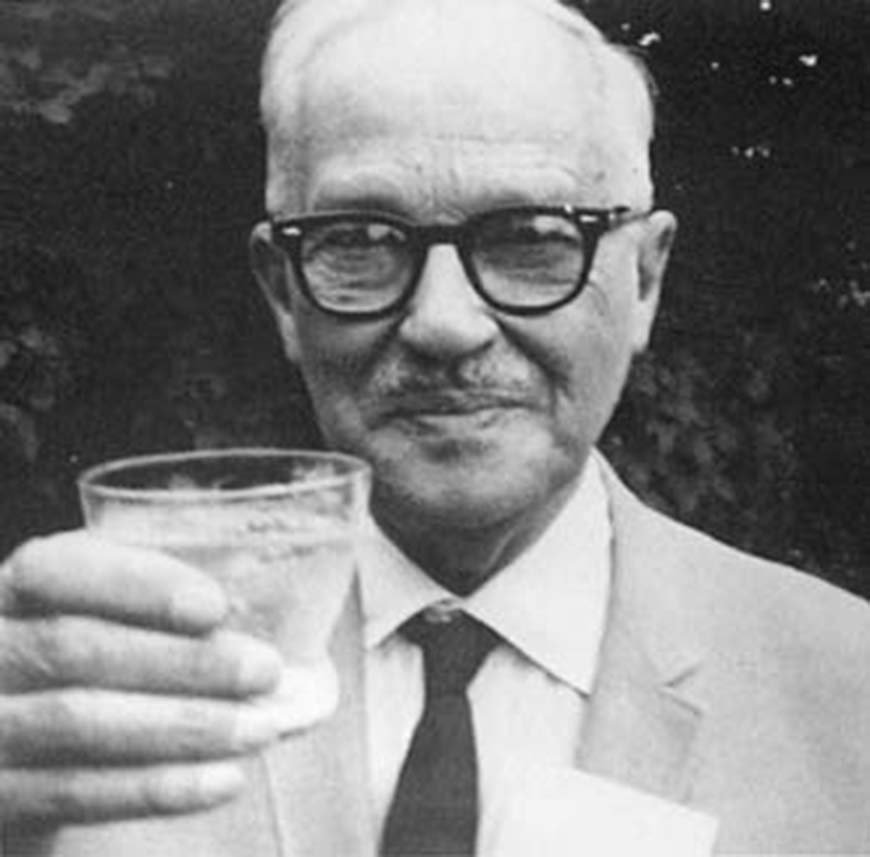
\includegraphics[width=0.9\columnwidth]{neyman.jpeg}
		\end{column}
	\end{columns}
\end{frame}

\begin{frame}{O que são Intervalos de Confiança?}
	\begin{exemplo}[Intervalo de Confiança de uma Política Pública]
		Digamos que você executou uma análise estatística para comparar
		eficácia de uma política pública em dois grupos e você obteve a
		diferença entre a média desses grupos. Você pode expressar essa
		diferença como um intervalo de confiança. Geralmente escolhemos a
		confiança de 95\%. Isso quer dizer que \textbf{95 estudos de 100},
		que usem o \textbf{mesmo tamanho de amostra e população-alvo},
		aplicando o \textbf{mesmo teste estatístico}, esperarão encontrar
		um resultado de diferenças de média entre grupos entre o intervalo
		de confiança.
	\end{exemplo}
	\footnotesize \textcolor{red}{Não diz nada sobre a sua \textbf{população-alvo},
		mas sim sobre a sua \textbf{amostra} num processo maluco de \textbf{amostragem infinita}...}
\end{frame}

\begin{frame}{Intevalos de Confiança versus Intervalos da Posterior}
	\centering
	\begin{tikzpicture}
		\begin{axis}[every axis plot, line width=2pt,
				xmin=0, xmax=4,
				ymin=0, ymax=1.5,
				ylabel=\empty,
				xlabel={$\theta$},
				samples=200,
				axis x line*=bottom, % no box around the plot, only x and y axis
				axis y line*=left,
				enlarge x limits=true,
			] % extend the axes a bit

			\addplot [blue, domain=0:4, forget plot] {lognormal(0, 2)};
			\addplot+ [
				mark=none,
				area legend,
				line width=0pt,
				color=blue,
				fill=blue, fill opacity=0.5,
				domain=0.25950495026507125:3.8534910373715427
			]
			{lognormal(0, 2)} \closedcycle;
			\addlegendentry{50\% Posterior}
			\addplot[red, mark=none] (-0.09, 1.4739034450607542) to (0.09, 1.4739034450607542);
			\addlegendentry{MLE}
			\draw [red] (0,0) to (0, 1.4739034450607542);
		\end{axis}
	\end{tikzpicture}
\end{frame}

\begin{frame}{Intevalos de Confiança versus Intervalos da Posterior}
	\centering
	\begin{tikzpicture}
		\begin{axis}[every axis plot, line width=2pt,
				xmin=-3, xmax=14,
				%ymin=0, ymax=1.5,
				ylabel=\empty,
				xlabel={$\theta$},
				samples=200,
				axis x line*=bottom, % no box around the plot, only x and y axis
				axis y line*=left,
				enlarge x limits=true,
				%legend pos=outer north east, %there is one default value for the `legend pos' that is outside the axis
				%legend cell align=left, % so the legend looks a bit better
			] % extend the axes a bit

			\addplot [blue, domain=-3:14, forget plot] {sumtwonormals(2, 1, 0.6, 10, 1, 0.4)};
			\addplot+ [
				mark=none,
				area legend,
				line width=0pt,
				color=blue,
				fill=blue, fill opacity=0.5,
				domain=1.8:9.7
			]
			{sumtwonormals(2, 1, 0.6, 10, 1, 0.4)} \closedcycle;
			\addlegendentry{50\% Posterior}
			\addplot[red, mark=none] (1.5, 0.24) to (2.5, 0.24);
			\addlegendentry{MLE}
			\draw [red] (2,0) to (2, 0.24);
		\end{axis}
	\end{tikzpicture}
\end{frame}

\begin{frame}{Mas por quê eu nunca vejo estatística sem $p$-valor?}
	\begin{columns}
		\begin{column}{0.8\textwidth}
			Não tem como entendermos $p$-valores se não compreendermos as suas
			origens e trajetória histórica. A primeira menção do termo foi feita
			pelo estatístico Ronald Fisher em 1925 \parencite{fisher1925statistical}:
			\begin{quotation}
				[$p$-valor é] índice que mede a força da evidência contra a hipótese nula
			\end{quotation}
			\begin{vfilleditems}
				\item Para quantificar a força da evidência contra a hipótese nula, Fisher defendeu
				"$p<0.05$ como um nível padrão para concluir que há evidência contra a hipótese testada"
				\item "Não seremos frequentemente perdidos se traçarmos uma linha convencional de 0.05"
			\end{vfilleditems}
		\end{column}
		\begin{column}{0.2\textwidth}
			\centering
			\includegraphics[width=0.9\columnwidth]{fisher.jpg}
		\end{column}
	\end{columns}
\end{frame}

\begin{frame}{$p = 0.06$}
	\begin{vfilleditems}
		\item Como o $p$-valor é uma probabilidade, ele é uma quantidade contínua.
		\item Não há razão para diferenciarmos um $p$ de 0.049 contra um $p$ de 0.051.
		\item Robert Rosenthal, um psicólogo já dizia "Deus ama $p$ de 0.06 tanto quanto um $p$ de 0.05"~\parencite{rosnow1989statistical}.
	\end{vfilleditems}
\end{frame}

\begin{frame}{Mas por quê eu nunca ouvi falar de Estatística Bayesiana?\footnote{\textit{inverse probability} é como o teorema de Bayes era chamado no começo do século XX}}
	\begin{columns}
		\begin{column}{0.8\textwidth}
			\begin{quotation}
				… it will be sufficient … to reaffirm my personal conviction …
				that the theory of inverse probability is founded upon an error,
				and must be wholly rejected.
			\end{quotation}
			\vfill \vfill
			\textcite{fisher1925statistical}
		\end{column}
		\begin{column}{0.2\textwidth}
			\centering
			\includegraphics[width=0.9\columnwidth]{fisher.jpg}
		\end{column}
	\end{columns}
\end{frame}

\begin{frame}{Dentro de todo não Bayesiano há um Bayesiano querendo sair\footnote{Dennis Lindley "Inside every nonBayesian there is a Bayesian struggling to get out"}}
	\begin{columns}
		\begin{column}{0.8\textwidth}
			\begin{vfilleditems}
				\item No último ano de sua vida, Fisher publicou um artigo \parencite{fisherExamplesBayesMethod1962} examinando as possibilidades dos métodos Bayesianos, mas com as probabilidades a \textit{priori} a serem determinadas experimentalmente.
				\item Inclusive alguns autores especulam \parencite{jaynesProbabilityTheoryLogic2003} que se Fisher estivesse vivo hoje, ele provavelmente seria um "Bayesiano".
			\end{vfilleditems}
		\end{column}
		\begin{column}{0.2\textwidth}
			\centering
			\includegraphics[width=0.9\columnwidth]{fisher.jpg}
		\end{column}
	\end{columns}
\end{frame}

\subsection{Estatística Bayesiana}
\begin{frame}{Teorema de Bayes como Motor de Inferência}
	\footnotesize Agora que você já sabe o que é probabilidade e o que é o teorema de Bayes, vou propor o seguinte modelo:
	$$
		\underbrace{P(\theta \mid y)}_{\text{Posterior}} = \frac{\overbrace{P(y \mid  \theta)}^{\text{Verossimilhança}} \cdot \overbrace{P(\theta)}^{\textit{Priori}}}{\underbrace{P(y)}_{\text{Constante Normalizadora}}}
	$$
	\begin{vfilleditems}
		\item \footnotesize $\theta$ -- parâmetro(s) de interesse
		\item \footnotesize $y$ -- dados observados
		\item \footnotesize \textbf{\textit{Priori}}: probabilidade prévia do valor do(s) parâmetro(s)
		\item \footnotesize \textbf{Verossimilhança}: probabilidade dos dados observados condicionados aos valores do(s) parâmetro(s)
		\item \footnotesize \textbf{Posterior}: probabilidade posterior do valor do(s) parâmetros após observamos os dados $y$
		\item \footnotesize \textbf{Constante Normalizadora}: $P(y)$ não faz sentido intuitivo. Essa probabilidade é transformada e pode ser interepretada como algo que existe apenas para que o resultado de $P(y \mid \theta) P(\theta)$ seja algo entre 0 e 1 -- uma probabilidade válida.
	\end{vfilleditems}
\end{frame}

\begin{frame}{Teorema de Bayes como Motor de Inferência}
	A estatísica Bayesiana nos permite \textbf{quantificar diretamente a incerteza}
	relacionada ao valor de um ou mais parâmetros do nosso modelo condicionado aos
	dados observados. Isso é a \textbf{característica principal} da estatística
	Bayesiana. Pois estamos estimando diretamente $P(\theta \mid y)$ por meio do
	teorema de Bayes. A estimativa resultante é totalmente intuitiva:
	simplesmente quantifica a intercerteza que temos sobre o valor de um ou mais
	parâmetro condicionado nos dados, nos pressupostos do nosso modelo
	(verossimilhança) e na probabilidade prévia que temos sobre tais valores.
\end{frame}

\subsubsection{Vantagens da Estatísca Bayesiana}
\begin{frame}{Estatística Bayesiana vs Frequentista}
	%\begin{table}[h!]
	\small
	\begin{tabular}{|l|p{.3\textwidth}|p{.3\textwidth}|}
		\toprule
		                       & \textcolor{blue}{\textbf{Estatística Bayesiana}} & \textcolor{red}{\textbf{Estatística Frequentista}}                  \\ \midrule
		\textbf{Dados}         & Fixos –- Não Aleatórios                          & Incertos –- Aleatórios                                              \\ \midrule
		\textbf{Parâmetros}    & Incertos –- Aleatórios                           & Fixos –- Não Aleatórios                                             \\ \midrule
		\textbf{Inferência}    & Incerteza sobre o valor do parâmetro             & Incerteza sobre um processo de amostragem de uma população infinita \\ \midrule
		\textbf{Probabilidade} & Subjetiva                                        & Objetiva (mas com diversos pressupostos dos modelos)                \\ \midrule
		\textbf{Incerteza}     & Intervalo de Credibilidade –- $P(\theta \mid y)$ & Intervalo de Confiança –- $P(y \mid \theta)$                        \\
		\bottomrule
	\end{tabular}
	%\end{table}
\end{frame}

\begin{frame}{Vantagens da Estatística Bayesiana}
	\begin{vfilleditems}
		\item Abordagem Natural para expressar Incerteza
		\item Habilidade de incorporar Informações Prévias
		\item Maior Flexibilidade do Modelo
		\item Distribuição Posterior completa dos Parâmetros
		\item Propagação Natural da Incerteza
	\end{vfilleditems}
	\small \textbf{Principal Desvantagem}: Velocidade lenta de estimativa de modelos\footnote{\textit{e.g.} 30 segundos ao invés de 3 segundos na abordagem frequentista}
\end{frame}

\begin{frame}{O começo do fim da Estatística Frequentista}
	\begin{vfilleditems}
		\small
		\item Saiba que você está em um momento da história no qual a Estatística está passando por grandes mudanças
		\item Acredito que a estatística frequentista, em especial a maneira que qualificamos evidências e hipóteses
		com $p$-valores se transformará de maneira "significante".
		\item Há cinco anos atrás, a \textit{American Statistical Association} (ASA) publicou uma declaração sobre
		$p$-valores \parencite{Wasserstein2016}. A declaração diz exatamente o que falamos aqui: Os conceitos principais do teste de significância de hipótese nula e, em particular $p$-valores não conseguem prover o que os pesquisadores requerem deles. Apesar do que dizem muitos livros de estatística, materiais de ensinos e artigos publicados, $p$-valores abaixo de 0,05 não "provam" a realidade de nada. Nem, chegando a esse ponto, os $p$-valores acima de 0,05 refutam alguma coisa.
		\item A declaração da ASA tem mais de 3.600 citações provocando impacto relevante.
	\end{vfilleditems}
\end{frame}

\begin{frame}{O começo do fim da Estatística Frequentista}
	\begin{vfilleditems}
		\small
		\item Um simpósio internacional foi promovido em 2017 que originou uma edição especial de acesso aberto da
		\textit{The American Statistician} dedicada à maneiras práticas de abandonarmos $p < 0.05$
		\parencite{wassersteinMovingWorld052019}.
		\item Logo na sequência vieram mais tentativas e reivindicações.
		Em setembro de 2017, a \textit{Nature Human Behaviour} publicou um editorial propondo que o nível de
		significância do $p$-valor seja reduzido de $0.05$ para $0.005$ \parencite{benjaminRedefineStatisticalSignificance2018}
		Diversos autores, inclusive muitos estatísticos altamente influentes e importantes argumentaram que esse simples passo
		ajudaria a combater o problema da crise de replicabilidade da ciência, que muitos acreditam ser a principal
		consequência do uso abusivo de $p$-valores \parencite{Ioannidis2019}.
		\item Além disso, muitos foram um passo além e sugerem que a ciência descarte de uma vez por todas $p$-valores
		\parencite{ItTimeTalk2019,lakensJustifyYourAlpha2018}. Muitos sugerem (eu inclusive) que a principal ferramenta
		de inferência seja a estatística Bayesiana \parencite{amrheinScientistsRiseStatistical2019, Goodman1180, vandeschootBayesianStatisticsModelling2021}
	\end{vfilleditems}
\end{frame}

\section{Distribuições Probabilísticas}

\subsection{Leituras Recomendadas}
\begin{frame}{Distribuições Probabilísticas - Leituras Recomendadas}
	\begin{vfilleditems}
		\item \textcite{dekkingModernIntroductionProbability2010}
		\begin{vfilleditems}
			\item Capítulo 4: Discrete random variables
			\item Capítulo 5: Continuous random variables
		\end{vfilleditems}
		\item \textcite{betancourtProbabilisticBuildingBlocks2019}
		\item \textcite{storopoli2021estatisticabayesianaR} - Distribuições Estatísticas
	\end{vfilleditems}
\end{frame}

%--- Intro -----------------------------------------------------------%
\begin{frame}{Distribuições Probabilísticas}
	A estatística Bayesiana usa distribuições probabilísticas como o motor de sua inferência na elaboração dos
	valores dos parâmetros estimados e suas incertezas.
	\vfill
	Imagine que distribuição probabilísticas são pequenas peças de "Lego". Podemos construir o que quisermos com
	essas pequenas peças. Podemos fazer um castelo, uma casa, uma cidade; literalmente o que quisermos. O mesmo é
	válido para modelos probabilísticos em estatística Bayesiana. Podemos construir modelos dos mais simples aos mais
	complexo a partir de distribuições probabilísticas e suas relações entre si.
\end{frame}

\begin{frame}{Distribuições Probabilísticas}
	\begin{defn}[Função de Distribuição de Probabilidade]
		Uma função de distribuição de probabilidade é a função matemática que fornece as probabilidades de ocorrência
		de diferentes resultados possíveis para um experimento. É uma descrição matemática de um fenômeno
		aleatório em termos de seu espaço amostral e as probabilidades de eventos (subconjuntos do espaço amostral).
		$$P(X): X \to \mathbb{R} \in [0, 1]$$
		Para variáveis discretas chamamos de "massa"~
		e para variáveis contínuas chamamos de "densidade".
	\end{defn}
\end{frame}

\begin{frame}{Notação Matemática}
	Geralmente usamos a notação
	$$X \sim \text{Dist}(\theta_1, \theta_2, \dots)$$
	Onde:
	\begin{vfilleditems}
		\item $X$: variável
		\item Dist: é o nome da distribuição
		\item $\theta_1, \theta_2, \dots$: os parâmetros que definem como a distribuição se comporta.
	\end{vfilleditems}
	Toda distribuição probabilística pode ser "parameterizada"~ao especificarmos parâmetros que permitem moldarmos alguns aspectos da distribuição para algum fim específico.
\end{frame}

\begin{frame}{Função Distribuição de Probabilidade}
	\centering
	\begin{tikzpicture}
		\begin{axis}[every axis plot, line width=2pt,
				ylabel=FDP,
				xlabel={$X$},
				domain=-4:4,samples=200,
				axis x line*=bottom, % no box around the plot, only x and y axis
				axis y line*=left, % the * suppresses the arrow tips
				enlarge x limits=true, % extend the axes a bit
			]

			\addplot [blue] {gaussian(0, 1)};
		\end{axis}
	\end{tikzpicture}
\end{frame}

\begin{frame}{Distribuições Probabilísticas}
	\begin{defn}[Função de Distribuição Cumulativa]
		A função de distribuição cumulativa (\textit{cumulative distribution function} - CDF)
		de uma variável aleatória $X$ avaliada em $x$ é a probabilidade que $X$ tomará
		valores menores ou iguais à $x$:
		$$\text{CDF} = P(X \leq x)$$
	\end{defn}
\end{frame}

\begin{frame}{Função de Distribuição Cumulativa}
	\centering
	\begin{tikzpicture}
		\begin{axis}[every axis plot, line width=2pt,
				ylabel=CDF,
				xlabel={$X$},
				domain=-4:4,samples=200,
				axis x line*=bottom, % no box around the plot, only x and y axis
				axis y line*=left, % the * suppresses the arrow tips
				enlarge x limits=true, % extend the axes a bit
			]

			\addplot [blue] {normcdf(0, 1)};
		\end{axis}
	\end{tikzpicture}
\end{frame}

%--- Discrete --------------------------------------------------------%
\subsection{Distribuições Discretas}
\begin{frame}{Distribuições Discretas}
	\begin{defn}[Distribuição de Probabilidade Discreta]
		Distribuições de probabilidade discretas são aquelas que os resultados são números
		discretos: $-N, \dots, -2, 1, 0,1,2,\dots, N$ e $N \in \mathbb{Z}$. Em distribuições discretas chamamos a
		probabilidade de uma distribuição tomar certos valores como "massa". A função massa de probabilidade
		$\text{FMP}$ é a função que especifica a probabilidade da variável aleatória $X$ tomar o valor $x$:
		$$\text{FMP}(x) = P(X = x)$$
	\end{defn}
\end{frame}

\subsubsection{Uniforme Discreta}
\begin{frame}{Uniforme Discreta}
	A distribuição uniforme discreta é uma distribuição de probabilidade simétrica em que um número finito de valores
	são igualmente prováveis de serem observados. Cada um dos $n$ valores tem probabilidade igual $\frac{1}{n}$.
	\vfill
	A distribuição uniforme discreta possui dois parâmetros e sua notação é $\text{Unif}(a, b)$:
	\begin{vfilleditems}
		\item Limite Inferior ($a$)
		\item Limite Superior ($b$)
	\end{vfilleditems}
	\vfill
	Exemplo: Um dado.
\end{frame}

\begin{frame}{Uniforme Discreta}
	$$\text{Unif}(a,b) = f(x, a, b) = \frac{1}{b-a+1} \quad \text{para $a \leq x \leq b$ e $x\in \{a,a+1,\dots ,b-1,b\}$}$$
\end{frame}

\begin{frame}{Uniforme Discreta}
	\centering
	\begin{tikzpicture}
		\begin{axis}[every axis plot,
				ybar=0pt, bar width=0.3,
				ylabel=PMF,
				samples at={1,...,6}, % All plots: from 1:6, 6 samples only
				axis x line*=bottom, % no box around the plot, only x and y axis
				axis y line*=left, % the * suppresses the arrow tips
				enlarge x limits=true, % extend the axes a bit
			]

			\addplot [fill=blue] {discreteuniform(1, 6)};
			\addlegendentry{$a=1, b=6$}
		\end{axis}
	\end{tikzpicture}
\end{frame}

\subsubsection{Bernoulli}
\begin{frame}{Bernoulli}
	A distribuição de Bernoulli descreve um evento binário de um sucesso de um experimento.
	Geralmente representamos $0$ como falha e $1$ como sucesso, então o resultado de uma distribuição de Bernoulli é
	uma variável binária $Y \in \{0, 1\}$.
	\vfill
	A distribuição de Bernoulli é muito usada para modelar resultados discretos binários no qual só há dois possíveis resultados.
	\vfill
	A distribuição de Bernoulli possui apenas um único paramêtro e sua notação é $\text{Bernoulli} (p)$:
	\begin{vfilleditems}
		\item Probabilidade de Sucesso ($p$)
	\end{vfilleditems}
	\vfill
	Exemplo: Se o paciente sobreviveu ou morreu ou se o cliente conclui sua compra ou não.
\end{frame}

\begin{frame}{Bernoulli}
	$$\text{Bernoulli}(p) = f(x, p)=p^{x}(1-p)^{1-x} \quad \text{para $x \in \{0,1\}$}$$ %
\end{frame}

\begin{frame}{Bernoulli}
	\centering
	\begin{tikzpicture}
		\begin{axis}[every axis plot,
				ybar=0pt, bar width=0.5,
				ymin=0,
				xmin=-0.25, xmax=1.25,
				ylabel=PMF,
				axis x line*=bottom, % no box around the plot, only x and y axis
				axis y line*=left, % the * suppresses the arrow tips
				enlarge x limits=true, % extend the axes a bit
				xtick={0, 1}
			]

			\addplot [fill=blue] coordinates {
					(0, 0.6)
					(1, 0.4)};
			\addlegendentry{$p=\frac{1}{3}$}
		\end{axis}
	\end{tikzpicture}
\end{frame}

\subsubsection{Binomial}
\begin{frame}{Binomial}
	A distribuição binomial descreve um evento do número de sucessos em uma sequência de $n$ experimentos independentes,
	cada um fazendo uma pergunta sim-não com probabilidade de sucesso $p$. Note que a distribuição de Bernoulli é
	um caso especial da distribuição binomial no qual o número de experimentos é $1$.
	\vfill
	A distribuição binomial possui dois parâmetros e sua notação é $\text{Bin}(n, p)$ ou $\text{Binomial}(n, p)$:
	\begin{vfilleditems}
		\item Número de Experimentos ($n$)
		\item Probabilidade de Sucessos ($p$)
	\end{vfilleditems}
	\vfill
	Exemplo: quantidade de caras em 5 lançamentos de uma moeda.
\end{frame}

\begin{frame}{Binomial}
	$$\text{Binomial}(n,p) = f(x, n, p) = \binom{n}{x}p^{x}(1-p)^{n-x} \quad \text{para $x \in \{0, 1, \dots, n\}$}$$
\end{frame}

\begin{frame}{Binomial}
	\centering
	\begin{tikzpicture}
		\begin{axis}[every axis plot,
				ybar=0pt, bar width=1,
				ylabel=PMF,
				ytick={0,0.05,...,0.15},
				samples at={0,...,40},
				axis x line*=bottom, % no box around the plot, only x and y axis
				axis y line*=left, % the * suppresses the arrow tips
				enlarge x limits=true, % extend the axes a bit
				y tick label style={/pgf/number format/.cd, fixed, fixed zerofill, precision=2}
			]

			\addplot [fill=blue, fill opacity=0.5] {binomial(40, 0.2)};
			\addlegendentry{$n=40, p=\frac{1}{5}$}
			\addplot [fill=red, fill opacity=0.5] {binomial(40, 0.5)};
			\addlegendentry{$n=40, p=\frac{1}{2}$}
		\end{axis}
	\end{tikzpicture}
\end{frame}

\subsubsection{Poisson}
\begin{frame}{Poisson}
	A distribuição Poisson expressa a probabilidade de um determinado número de
	eventos ocorrerem em um intervalo fixo de tempo ou espaço se esses eventos
	ocorrerem com uma taxa média constante conhecida e independentemente do tempo
	desde o último evento. A distribuição de Poisson também pode ser usada
	para o número de eventos em outros intervalos especificados, como distância,
	área ou volume.
	\vfill
	A distribuição Poisson possui um parâmetro e sua notação é $\text{Poisson}(\lambda)$:
	\begin{vfilleditems}
		\item Taxa ($\lambda$)
	\end{vfilleditems}
	\vfill
	Exemplo: Quantidade de e-mails que você recebe diariamente. Quantidade de buracos que você encontra na rua.
\end{frame}

\begin{frame}{Poisson}
	$$\text{Poisson}(\lambda) = f(x, \lambda) = \frac{\lambda^x e^{-\lambda}}{x!} \quad \text{para $\lambda > 0$}$$
\end{frame}

\begin{frame}{Poisson}
	\centering
	\begin{tikzpicture}
		\begin{axis}[every axis plot,
				ybar=0pt, bar width=1,
				ylabel=PMF,
				samples at={0,...,8},
				axis x line*=bottom, % no box around the plot, only x and y axis
				axis y line*=left, % the * suppresses the arrow tips
				enlarge x limits=true, % extend the axes a bit
			]

			\addplot [fill=blue, fill opacity=0.5] {poisson(1)};
			\addlegendentry{$\lambda=2$}
			\addplot [fill=red, fill opacity=0.5] {poisson(4)};
			\addlegendentry{$\lambda=4$}
		\end{axis}
	\end{tikzpicture}
\end{frame}

\subsubsection{Binomial Negativa}
\begin{frame}{Binomial Negativa\footnote{Qualquer fenômeno que pode ser modelo com uma distribuição de Poisson, pode ser modelo com uma distribuição binomial negativa \parencite{gelman2013bayesian, gelman2020regression}.}}
	\small
	A distribuição binomial negativa descreve um evento do número de sucessos em uma
	sequência de $n$ experimentos independentes, cada um fazendo uma pergunta sim-não
	com probabilidade $p$ até que se obtenha $k$ sucessos. Note que ela se torna
	idêntica à distribuição de Poisson quando no limite de $k \to \infty$. Isto faz
	com que seja uma opção robusta para substituir uma distribuição de Poisson para
	modelar fenômenos com uma \textit{superdispersão} (variação nos dados excedente ao
	esperado).
	\vfill \small
	A distribuição negativa binomial possui dois parâmetros e sua notação é
	$\text{Binomial Negativa}(k, p)$:
	\begin{vfilleditems}
		\small
		\item Número de Sucessos ($k$)
		\item Probabilidade de Sucessos ($p$)
	\end{vfilleditems}
	\vfil \small
	Exemplo: Contagem anual de ciclones tropicais.
\end{frame}

\begin{frame}{Binomial Negativa}
	$$
		\begin{aligned}
			\text{Binomial Negativa}(k, p) & = f(x, k, p) & = \binom{x + k - 1}{k - 1}p^{x}(1-p)^{k} \\
			\\
			                               & ~            & \text{para $x \in \{0, 1, \dots, n\}$}
		\end{aligned}
	$$
\end{frame}

\begin{frame}{Binomial Negativa}
	\centering
	\begin{tikzpicture}
		\begin{axis}[every axis plot,
				ybar=0pt, bar width=1,
				ylabel=PMF,
				samples at={0,...,8},
				axis x line*=bottom, % no box around the plot, only x and y axis
				axis y line*=left, % the * suppresses the arrow tips
				enlarge x limits=true, % extend the axes a bit
			]

			\addplot [fill=blue, fill opacity=0.5] {negativebinomial(1, 0.5)};
			\addlegendentry{$k=1, p=\frac{1}{2}$}
			\addplot [fill=red, fill opacity=0.5] {negativebinomial(5,0.5)};
			\addlegendentry{$k=5, p=\frac{1}{2}$}
		\end{axis}
	\end{tikzpicture}
\end{frame}

%--- Continuous ------------------------------------------------------%

\subsection{Distribuições Contínuas}
\begin{frame}{Distribuições Contínuas}
	\begin{defn}[Distribuição de Probabilidade Contínua]
		\small
		Distribuições de probabilidade contínuas são aquelas que os resultados
		são valores em uma faixa contínua (também chamados de número reais):
		$(-\infty, +\infty) \in \mathbb{R}$.
		Em distribuições contínuas chamamos a probabilidade de uma distribuição
		tomar certos valores como "densidade". Como estamos falando sobre
		números reais não conseguimos obter a probabilidade de uma variável aleatória
		$X$ tomar o valor de $x$. Isto sempre será $0$, pois não há como especificar
		um valor exato de $x$. $x$ vive na linha dos números reais, portanto,
		precisamos especificar a probabilidade de $X$ tomar valores em um \textbf{intervalo}
		$[a,b]$. A função densidade de probabilidade $\text{FDP}$ é definida como:
		$$\text{FDP}(x) = P(a \leq X \leq b) = \int_a^b f(x) dx$$
	\end{defn}
\end{frame}

\subsubsection{Uniforme Contínua}
\begin{frame}{Uniforme Contínua}
	A distribuição uniforme contínua é uma distribuição de probabilidade simétrica em que um número infinito de intervalos de valores
	são igualmente prováveis de serem observados. Cada um dos $n$ infinitos intervalos valores tem probabilidade igual $\frac{1}{n}$.
	\vfill
	A distribuição uniforme contínua possui dois parâmetros e sua notação é $\text{Unif}(a, b)$:
	\begin{vfilleditems}
		\item Limite Inferior ($a$)
		\item Limite Superior ($b$)
	\end{vfilleditems}
\end{frame}

\begin{frame}{Uniforme Contínua}
	$$\text{Unif}(a,b) = f(x, a, b) = \frac{1}{b-a} \quad \text{para $a \leq x \leq b$ e $x \in [a, b]$}$$
\end{frame}

\begin{frame}{Uniforme Contínua}
	\centering
	\begin{tikzpicture}
		\begin{axis}[every axis plot, line width=2pt,
				ylabel=PDF,
				domain=0:6,samples=200,
				axis x line*=bottom, % no box around the plot, only x and y axis
				axis y line*=left, % the * suppresses the arrow tips
				enlarge x limits=true, % extend the axes a bit
			]

			\addplot [blue] {continuousuniform(0, 6)};
			\addlegendentry{$a=0, b=6$}
		\end{axis}
	\end{tikzpicture}
\end{frame}

\subsubsection{Normal}
\begin{frame}{Normal}
	Essa distribuição geralmente é usada nas ciências sociais e naturais para
	representar variáveis contínuas na qual as suas distribuições não são conhecidas.
	Esse pressuposto é por conta do teorema do limite central. O teorema do limite
	central afirma que, em algumas condições, a média de muitas amostras (observações)
	de uma variável aleatória com média e variância finitas é ela própria uma variável
	aleatória cuja distribuição converge para uma distribuição normal à medida que o
	número de amostras aumenta.
	\vfill
	Portanto, as quantidades físicas que se espera sejam a
	soma de muitos processos independentes (como erros de medição) muitas vezes têm
	distribuições que são quase normais.
\end{frame}

\begin{frame}{Normal}
	A distribuição normal possui dois parâmetros e sua notação é
	$\text{Normal}(\mu, \sigma^2)$ ou $\text{N}(\mu, \sigma^2)$:
	\begin{vfilleditems}
		\item Média ($\mu$): média da distribuição e também a moda e a mediana
		\item Desvio Padrão ($\sigma$) (às vezes também parametrizada com a variância $\sigma^2$): é uma medida de dispersão das observações em relação à média
	\end{vfilleditems}
	\vfill
	Exemplo: Altura, Peso etc.
\end{frame}

\begin{frame}{Normal\footnote{veja como a distribuição Normal foi derivada a partir da distribuição binomial nos \hyperlink{appendixnormal}{Slides de Backup no final dessa apresentação}}}
	$$\text{Normal}(\mu,\sigma) = f(x, \mu, \sigma) = \frac{1}{\sigma{\sqrt{2\pi }}}e^{-{\frac{1}{2}}\left({\frac {x-\mu }{\sigma }}\right)^{2}} \quad \text{para $\sigma > 0$}$$
\end{frame}

\begin{frame}{Normal}
	\centering
	\begin{tikzpicture}
		\begin{axis}[every axis plot, line width=2pt,
				ylabel=PDF,
				domain=-4:6,samples=200,
				axis x line*=bottom, % no box around the plot, only x and y axis
				axis y line*=left, % the * suppresses the arrow tips
				enlarge x limits=true, % extend the axes a bit
			]

			\addplot [blue] {gaussian(0, 1)};
			\addlegendentry{$\mu=0, \sigma=1$}
			\addplot [red] {gaussian(0, 2)};
			\addlegendentry{$\mu=0, \sigma=2$}
			\addplot [yellow] {gaussian(2, 1)};
			\addlegendentry{$\mu=2, \sigma=1$}
		\end{axis}
	\end{tikzpicture}
\end{frame}

\subsubsection{Log-Normal}
\begin{frame}{Log-Normal}
	A distribuição Log-normal é uma distribuição de probabilidade contínua de uma
	variável aleatória cujo logaritmo é normalmente distribuído. Assim, se a variável
	aleatória $X$ for distribuída normalmente por $\log$ natural ($\ln$),
	então $Y = \ln(X)$ terá uma distribuição normal.
	\vfill
	Uma variável aleatória com distribuição logarítmica aceita apenas valores reais
	positivos. É um modelo conveniente e útil para medições em ciências exatas e de
	engenharia, bem como medicina, economia e outros campos, por ex. para energias,
	concentrações, comprimentos, retornos financeiros e outros valores.
	\vfill
	Um processo log-normal é a realização estatística do produto multiplicativo de
	muitas variáveis aleatórias independentes, cada uma das quais positiva.
\end{frame}

\begin{frame}{Log-Normal}
	A distribuição log-normal possui dois parâmetros e sua notação é
	$\text{Log-Normal}(\mu, \sigma^2)$:
	\begin{vfilleditems}
		\item Média ($\mu$): média do logaritmo natural ($\ln$) da distribuição
		\item Desvio Padrão ($\sigma$): a variância do logaritmo natural da distribuição ($\sigma^2$) é uma medida de dispersão das observações em relação à média
	\end{vfilleditems}
\end{frame}

\begin{frame}{Log-Normal}
	$$\text{Log-Normal}(\mu,\sigma) = f(x, \mu, \sigma) = \frac{1}{x \sigma{\sqrt{2\pi}}}e^{-\left({\frac {(\ln(x)-\mu)^2}{2 \sigma^2 }}\right)} \quad \text{para $\sigma > 0$}$$
\end{frame}

\begin{frame}{Log-Normal}
	\centering
	\begin{tikzpicture}
		\begin{axis}[every axis plot, line width=2pt,
				ylabel=PDF,
				domain=0:5,samples=200,
				axis x line*=bottom, % no box around the plot, only x and y axis
				axis y line*=left, % the * suppresses the arrow tips
				enlarge x limits=true, % extend the axes a bit
			]

			\addplot [blue] {lognormal(0, 0.25)};
			\addlegendentry{$\mu=0, \sigma=\frac{1}{4}$}
			\addplot [red] {lognormal(0, 1)};
			\addlegendentry{$\mu=0, \sigma=1$}
			\addplot [yellow] {lognormal(1, 1)};
			\addlegendentry{$\mu=1, \sigma=1$}
		\end{axis}
	\end{tikzpicture}
\end{frame}

\subsubsection{Exponencial}
\begin{frame}{Exponencial}
	A distribuição exponencial é a distribuição de probabilidade do tempo entre
	eventos que ocorrem de forma contínua e independente a uma taxa média constante.
	\vfill
	A distribuição exponencial possui um parâmetro e sua notação é
	$\text{Exp}(\lambda)$:
	\begin{vfilleditems}
		\item Taxa ($\lambda$)
	\end{vfilleditems}
	\vfill
	Exemplo: Quanto tempo até o próximo terremoto. Quanto tempo até o próximo ônibus.
\end{frame}

\begin{frame}{Exponencial}
	$$\text{Exp}(\lambda) = f(x, \lambda) = \lambda e^{-\lambda x} \quad \text{para $\lambda > 0$}$$
\end{frame}

\begin{frame}{Exponencial}
	\centering
	\begin{tikzpicture}
		\begin{axis}[every axis plot, line width=2pt,
				ylabel=PDF,
				domain=0:5,samples=200,
				axis x line*=bottom, % no box around the plot, only x and y axis
				axis y line*=left, % the * suppresses the arrow tips
				enlarge x limits=true, % extend the axes a bit
			]

			\addplot [blue] {exponential(0.5)};
			\addlegendentry{$\lambda=\frac{1}{2}$}
			\addplot [red] {exponential(1)};
			\addlegendentry{$\lambda=1$}
			\addplot [yellow] {exponential(2)};
			\addlegendentry{$\lambda=2$}
		\end{axis}
	\end{tikzpicture}
\end{frame}

\subsubsection{$t$ de Student}
\begin{frame}{$t$ de Student}
	A distribuição $t$ de Student surge ao estimar a média de uma população
	normalmente distribuída em situações onde o tamanho da amostra é pequeno e o
	desvio padrão da população é
	desconhecido\footnote{Daqui que vem o tal do teste $t$ de Student}.
	\vfill
	Se tomarmos uma amostra de $n$ observações de uma distribuição normal,
	então a distribuição $t$ com $\nu = n-1$ graus de liberdade pode ser definida
	como a distribuição da localização da média da amostra em relação à média
	verdadeira, dividida pela desvio padrão da amostra, após multiplicar
	pelo termo padronizador $\sqrt{n}$.
	\vfill
	A distribuição $t$ é simétrica e em forma de sino, como a distribuição normal,
	mas tem caudas mais longas, o que significa que é mais propensa a produzir
	valores que estão longe de sua média.
\end{frame}

\begin{frame}{$t$ de Student}
	A distribuição $t$ de Student possui um parâmetro e sua notação é
	$\text{Student}(\nu)$:
	\begin{vfilleditems}
		\item Graus de Liberdade ($\nu$): controla o quanto ela se assemelha com uma distribuição normal
	\end{vfilleditems}
	\vfill
	Exemplo: Uma base de dados cheia de outliers.
\end{frame}

\begin{frame}{$t$ de Student}
	$$\text{Student}(\nu) = f(x, \nu) = \frac{\Gamma \left(\frac{\nu+1}{2} \right)} {\sqrt{\nu\pi}\,\Gamma \left(\frac{\nu}{2} \right)} \left(1+\frac{x^2}{\nu} \right)^{-\frac{\nu+1}{2}} \quad \text{para $\nu \geq 1$}$$
\end{frame}

\begin{frame}{$t$ de Student}
	\centering
	\begin{tikzpicture}
		\begin{axis}[every axis plot, line width=2pt,
				ylabel=PDF,
				domain=-4:4,samples=200,
				axis x line*=bottom, % no box around the plot, only x and y axis
				axis y line*=left, % the * suppresses the arrow tips
				enlarge x limits=true, % extend the axes a bit
			]

			\addplot [blue] {student(1)};
			\addlegendentry{$\nu=1$}
			\addplot [red] {student(3)};
			\addlegendentry{$\nu=3$}
			\addplot [yellow] {student(30)};
			\addlegendentry{$\nu=30$}
		\end{axis}
	\end{tikzpicture}
\end{frame}

\subsubsection{Beta}
\begin{frame}{Beta}
	A distribuição beta é uma escolha natural para modelar qualquer coisa
	que seja restrita a valores entre $0$ e $1$. Portanto, é uma boa candidata
	para probabilidades e proporções.
	\vfill
	A distribuição beta possui dois parâmetros e sua notação é $\text{Beta} (\alpha, \beta)$:
	\begin{vfilleditems}
		\item Parâmetro de Forma ($\alpha$ ou às vezes $a$): controla o quanto a forma é deslocada para próximo de $1$
		\item Parâmetro de Forma ($\beta$ ou às vezes $b$): controla o quanto a forma é deslocada para próximo de $0$
	\end{vfilleditems}
	\vfill
	Exemplo: Um jogador de basquete já marcou 5 lances livres e errou 3 em um
	total de 8 tentativas - $\text{Beta}(3, 5)$
\end{frame}

\begin{frame}{Beta}
	$$\text{Beta} (\alpha, \beta) = f(x, \alpha, \beta) \frac{x^{\alpha-1}(1-x)^{\beta-1}} {\frac{\Gamma (\alpha )\Gamma (\beta )}{\Gamma (\alpha +\beta )}} \quad \text{para $\alpha,\beta > 0$ e $x \in [0, 1]$}$$
\end{frame}

\begin{frame}{Beta}
	\centering
	\begin{tikzpicture}
		\begin{axis}[every axis plot, line width=2pt,
				ylabel=PDF,
				domain=0:1,samples=200,
				axis x line*=bottom, % no box around the plot, only x and y axis
				axis y line*=left, % the * suppresses the arrow tips
				enlarge x limits=true, % extend the axes a bit
			]

			\addplot [blue] {beta(1,1)};
			\addlegendentry{$\alpha=\beta=1$}
			\addplot [red] {beta(3,2)};
			\addlegendentry{$\alpha=3,\beta=2$}
			\addplot [yellow] {beta(2,3)};
			\addlegendentry{$\alpha=2,\beta=3$}
		\end{axis}
	\end{tikzpicture}
\end{frame}

\section{\texttt{rstanarm} e \texttt{brms}}

\subsection{Leituras Recomendadas}
\begin{frame}{\texttt{rstanarm} e \texttt{brms} - Leituras Recomendadas\footnote{\texttt{rstanarm} - \url{http://mc-stan.org/rstanarm/} e \texttt{brms} - \url{https://paul-buerkner.github.io/brms/}}}
	\begin{vfilleditems}
		\item Vinheta e Manual do \texttt{rstanarm} de \textcite{rstanarm}
		\item Vinheta e Manual do \texttt{brms} de \textcite{brms}
		\item Tutorial de \texttt{rstanarm} de \textcite{muth2018user}
		\item Tutorial de \texttt{brms} de \textcite{burknerAdvancedBayesianMultilevel2018}
		\item \textit{Workflow} Bayesiano de \textcite{gelmanBayesianWorkflow2020}
		\item \textit{Workflow} Visual Bayesiano de \textcite{gabryVisualizationBayesianWorkflow2019}
		\item Vinheta e Manual do \texttt{bayesplot} \textcite{bayesplot}
		\item \textcite{storopoli2021estatisticabayesianaR} - \texttt{rstanarm} e \texttt{brms}
	\end{vfilleditems}
\end{frame}

\subsection{Ecosistema \texttt{Stan}}
\begin{frame}{O que é \href{https://mc-stan.org}{\texttt{Stan}}}
	\begin{columns}
		\begin{column}{0.8\textwidth}
			\href{https://mc-stan.org}{\texttt{Stan}}
			\parencite{carpenterStanProbabilisticProgramming2017} é uma \textbf{plataforma para
				modelagem e computação estatística de alto desempenho}.
			Milhares de usuários contam com \texttt{Stan} para modelagem estatística,
			análise de dados e previsão nas ciências sociais, biológicas e físicas,
			engenharia e negócios.
		\end{column}
		\begin{column}{0.2\textwidth}
			\centering
			\includegraphics[width=0.6\textwidth]{stan_transparent.png}
		\end{column}
	\end{columns}
\end{frame}

\subsubsection{Interfaces Oficiais}
\begin{frame}{Interfaces do \href{https://mc-stan.org}{\texttt{Stan}}}
	\begin{vfilleditems}
		\item \texttt{R}: \href{https://mc-stan.org/users/interfaces/rstan.html}{\texttt{RStan}} e \href{https://mc-stan.org/cmdstanr}{\texttt{CmdStanR}}
		\item Python: \href{https://mc-stan.org/users/interfaces/pystan.html}{\texttt{PyStan}} e \href{https://cmdstanpy.readthedocs.io/en/latest/getting_started.html}{\texttt{CmdStanPy}}
		\item \texttt{Shell} (Linha de Comando): \href{https://mc-stan.org/users/interfaces/cmdstan.html}{\texttt{CmdStan}}
		\item \texttt{Julia}: \href{https://mc-stan.org/users/interfaces/julia-stan.html}{\texttt{Stan.jl}}
		\item \texttt{Scala}: \href{https://github.com/cibotech/ScalaStan}{\texttt{ScalaStan}}
		\item \sout{\texttt{Matlab}}: \href{https://mc-stan.org/users/interfaces/matlab-stan.html}{\sout{\texttt{MatlabStan}}}
		\item \sout{\texttt{Stata}}: \href{https://mc-stan.org/users/interfaces/stata-stan.html}{\sout{\texttt{StataStan}}}
		\item \sout{\texttt{Mathematica}}: \href{https://mc-stan.org/users/interfaces/mathematica-stan.html}{\sout{\texttt{MathematicaStan}}}
	\end{vfilleditems}
\end{frame}

\begin{frame}{Interfaces Amigáveis do \href{https://mc-stan.org}{\texttt{Stan}}}
	Somente para \texttt{R}
	\begin{columns}
		\begin{column}{0.8\textwidth}
			\begin{vfilleditems}
				\item \href{http://mc-stan.org/rstanarm/}{\texttt{rstanarm}} \parencite{rstanarm}: ajuda o usuário a especificar modelos usando a sintaxe familiar de fórmulas do \texttt{R}.
				\item \href{https://paul-buerkner.github.io/brms/}{\texttt{brms}} \parencite{brms}: similar ao \texttt{rstanarm} pois usa a sintaxe familiar de fórmulas do \texttt{R}, mas dá maior flexibilidade na especificação de modelos mais complexos.
			\end{vfilleditems}
		\end{column}
		\begin{column}{0.2\textwidth}
			\centering
			\includegraphics[width=0.6\textwidth]{brms.png}
		\end{column}
	\end{columns}
\end{frame}

\begin{frame}[fragile]{Código \href{https://mc-stan.org}{\texttt{Stan}}}
	\begin{lstlisting}[basicstyle=\small, language=Stan]
    data {
      int<lower=0> N;
      vector[N] x1;
      vector[N] x2;
      vector[N] y;
    }
    parameters {
      real alpha;
      vector[2] beta;
      real<lower=0> sigma;
    }
    model {
      sigma ~ cauchy(0, 2.5);
      y ~ normal(alpha + beta[1] * x1 + beta[2] * x2, sigma);
    }
    \end{lstlisting}
\end{frame}

\begin{frame}{\href{http://mc-stan.org/rstanarm/}{\texttt{rstanarm}} versus \href{https://paul-buerkner.github.io/brms/}{\texttt{brms}}}
	Para remediar essa barreira de acesso ao \href{https://mc-stan.org}{\texttt{Stan}},
	temos interfaces abstratas que interpretam a intenção do usuário e
	lidam com a parte mais \textit{obral} de codificação:
	\begin{vfilleditems}
		\small
		\item \href{http://mc-stan.org/rstanarm/}{\texttt{rstanarm}} todos os
		modelos são pré-compilados e
		\href{https://paul-buerkner.github.io/brms/}{\texttt{brms}} não possui os
		modelos pré-compilados então os modelos devem ser todos compilados antes de serem rodados
		\item Como \href{https://paul-buerkner.github.io/brms/}{\texttt{brms}}
		compila os modelos conforme a especificação do usuário, ele pode criar
		modelos um pouco mais eficientes que o \href{http://mc-stan.org/rstanarm/}{\texttt{rstanarm}}
		\item \href{https://paul-buerkner.github.io/brms/}{\texttt{brms}} dá maior poder e flexibilidade
		ao usuário na especificação de funções de verossimilhança e também permite modelos mais complexos
		que o \href{http://mc-stan.org/rstanarm/}{\texttt{rstanarm}}
	\end{vfilleditems}
\end{frame}

\subsubsection{Pacotes}
\begin{frame}{Pacotes \texttt{R}}
	\begin{columns}
		\begin{column}{0.5\textwidth}
			\begin{vfilleditems}
				\item \href{https://mc-stan.org/bayesplot/}{\texttt{bayesplot}} -- visualização
				\item \href{http://mc-stan.org/loo/}{\texttt{loo}} -- seleção de modelos com LOO-CV
				\item \href{https://mc-stan.org/projpred/}{\texttt{projpred}} -- seleção de variáveis
				\item \href{https://facebook.github.io/prophet/}{\texttt{prophet}} -- previsão de séries temporais
				\item \href{https://github.com/asael697/varstan}{\texttt{varstan}} -- modelos \textit{Vector Auto-Regressive} (VAR)
			\end{vfilleditems}
		\end{column}
		\begin{column}{0.5\textwidth}
			\begin{vfilleditems}
				\item \href{https://github.com/ecmerkle/blavaan}{\texttt{blavaan}} -- \textit{Structural Equation Modeling} (SEM)
				\item \href{https://github.com/jtimonen/lgpr/}{\texttt{lgpr}} -- \textit{Longitudinal Gaussian Process Regression} (LGPR)
				\item \href{https://github.com/asael697/bayesforecast}{\texttt{bayesforecast}} -- previsão de séries temporais
				\item \href{https://github.com/wwiecek/baggr}{\texttt{baggr}} -- meta-análise
				\item \href{https://github.com/macartan/CausalQueries}{\texttt{CausalQueries}} -- modelos binários causais
			\end{vfilleditems}
		\end{column}
	\end{columns}
\end{frame}

\begin{frame}{\href{https://mc-stan.org}{\texttt{Stan}}\footnote{foi lançado em 2012} na Scopus\footnote{veja as buscas Scopus nos \hyperlink{appendixscopus}{Slides de Backup no final dessa apresentação}}}
	\centering
	\begin{tikzpicture}[ybar]
		\begin{axis}[
				xlabel=Ano,ylabel=Uso,
				x tick label style={rotate=45, /pgf/number format/.cd,
						scaled x ticks = false,
						set thousands separator={},
						fixed}]
			\addplot [draw=blue, fill=blue] coordinates {
					(2012, 6)
					(2013, 19)
					(2014, 62)
					(2015, 113)
					(2016, 189)
					(2017, 387)
					(2018, 671)
					(2019, 1045)
					(2020, 1538)
				};
		\end{axis}
	\end{tikzpicture}
\end{frame}

\begin{frame}{\href{https://mc-stan.org}{\texttt{Stan}}\footnote{baseado no \href{https://breckbaldwin.github.io/ScientificSoftwareImpactMetrics/DeepLearningAndBayesianSoftware.html}{reporte anual do Breck Baldwin para a NUMFocus}}\footnote{veja as buscas Scopus nos \hyperlink{appendixscopus}{Slides de Backup no final dessa apresentação}}}
	\centering
	\begin{tikzpicture}[ybar]
		\begin{axis}[
				nodes near coords={\pgfmathprintnumber[fixed,precision=3]{\pgfplotspointmeta}},
				ylabel=Uso, xtick={1,2,3,4},
				ymax=0.85,
				ytick={0.1, 0.2, 0.3, 0.4, 0.5, 0.6, 0.7, 0.8},
				xticklabels={\texttt{TensorFlow}, \texttt{PyTorch}, \texttt{Stan}, \texttt{PyMC}}]
			\addplot [draw=yellow, fill=yellow] coordinates {
					(1, 0.713)};
			\addplot [draw=green, fill=green] coordinates {
					(2, 0.161)};
			\addplot [draw=blue, fill=blue] coordinates {
					(3, 0.108)};
			\addplot [draw=red, fill=red] coordinates {
					(4, 0.0176)};
		\end{axis}
	\end{tikzpicture}
\end{frame}

\subsection{Especificação de Modelos com Fórmulas}
\begin{frame}[fragile]{Especificação de Modelos com Fórmulas}
	Todos os modelos especificados pelo \href{http://mc-stan.org/rstanarm/}{\texttt{rstanarm}}
	e \href{https://paul-buerkner.github.io/brms/}{\texttt{brms}} usam uma fórmula
	com a seguinte síntaxe:
	\vfill
	\begin{lstlisting}
    dependente ~ independente_1 + independente_2 + ...
    \end{lstlisting}
\end{frame}

\begin{frame}[fragile]{Especificação de Modelos com Fórmulas}
	Moderações?! Sem problema:
	\vfill
	\begin{lstlisting}[basicstyle=\footnotesize]
dependente ~ independente_1 * moderadora + independente_2 * moderadora + ...
    \end{lstlisting}
\end{frame}

\subsection{Funções de Verossimilhança com \texttt{family}}
\begin{frame}{Funções de Verossimilhança com \texttt{family}}
	Todo modelo especificado pelo \href{http://mc-stan.org/rstanarm/}{\texttt{rstanarm}} e
	\href{https://paul-buerkner.github.io/brms/}{\texttt{brms}} devem especificar qual
	família da função de verossimilhança (\texttt{family}) respectivamente com a
	função de ligação (\texttt{link}) que fará o mapeamento dos parâmetros
	condicionados nos dados para a variável
	dependente\footnote{caso o usuário não designe nenhum valor para esses dois parâmetros, \href{http://mc-stan.org/rstanarm/}{\texttt{rstanarm}} e \href{https://paul-buerkner.github.io/brms/}{\texttt{brms}} usarão a verossimilhança Gaussiana (\texttt{family = gaussian}) e a função de identidade como função de ligação (\texttt{link = "identity"})}.
\end{frame}

\begin{frame}{Funções de Verossimilhança com \texttt{family}}
	\begin{vfilleditems}
		\item Gaussiana -- \texttt{family = gaussian(link = "identity")}
		\item Log-Normal -- \texttt{family = lognormal(link = "log")}
		\item Binomial -- \texttt{family = binomial(link = "logit")}
		\item Poisson -- \texttt{family = poisson(link = "log")}
		\item Binomial Negativa -- \texttt{family = negbinomial(link = "log")}
		\item $t$ de Student -- \texttt{family = student(link = "identity")}
		\item Exponencial -- \texttt{family = exponential(link = "log")}
	\end{vfilleditems}
\end{frame}

\subsection{\texttt{rstanarm}}

\begin{frame}{\href{http://mc-stan.org/rstanarm/}{\texttt{rstanarm}}\footnote{\textcite{rstanarm}}}
	O \href{http://mc-stan.org/rstanarm/}{\texttt{rstanarm}} é a porta de
	entrada para estatística Bayesiana com \href{https://mc-stan.org}{\texttt{Stan}}.
	\vfill
	O nome \texttt{rstanarm} é:
	\begin{vfilleditems}
		\item \texttt{r}: pacote para \texttt{R}
		\item \texttt{stan}: usa a linguagem probabilística \texttt{Stan}
		\item \texttt{arm}: acrônimo para \textit{Applied Regression Modeling}
	\end{vfilleditems}
\end{frame}

\subsubsection{Modelos do \texttt{rstanarm}}
\begin{frame}{Modelos do \href{http://mc-stan.org/rstanarm/}{\texttt{rstanarm}}\footnote{Neste curso usaremos apenas \texttt{stan\_glm} e \texttt{stan\_glmer}, mas saiba que você possui uma vasta categoria de modelos Bayesianos à disposição}}
	\begin{vfilleditems}
		\item \texttt{stan\_glm()} -- modelos lineares generalizados (\textit{\textbf{g}eneralized \textbf{l}inear \textbf{m}odel})
		\item \texttt{stan\_lm()} -- modelos lineares regularizados (\textit{\textbf{l}inear \textbf{m}odel)}
		\item \texttt{stan\_aov()} -- modelo ANOVA (\textit{\textbf{an}alysis \textbf{o}f \textbf{va}riance})
		\item \texttt{stan\_glmer()} - modelos linares generalizados multiníveis
		\item \texttt{stan\_lmer()} -- modelos linares regularizados multiníveis
		\item \texttt{stan\_jm()} -- modelos longitudinais e de sobrevivência
		\item \texttt{stan\_nlmer()} -- modelos não-lineares multiníveis (\textit{\textbf{n}on-\textbf{l}inear \textbf{m}odel})
		\item \texttt{stan\_polr()} -- modelos ordinais
		\item \texttt{stan\_gamm4()} -- modelos aditivos linares multiníveis
	\end{vfilleditems}
\end{frame}

\begin{frame}[fragile]{Exemplo Simples do \href{http://mc-stan.org/rstanarm/}{\texttt{rstanarm}}}
	\begin{lstlisting}
    library(rstanarm)
    rstanarm_fit <- @stan_glm(mpg ~ wt + am, data = mtcars)@
    summary(rstanarm_fit)
    \end{lstlisting}
\end{frame}

\begin{frame}{\texttt{summary} do \href{http://mc-stan.org/rstanarm/}{\texttt{rstanarm}}}
	\centering
	\begin{tabular}{lrrrrrrr}
		\toprule
		Parameter   & Rhat & n\_eff & mean  & sd   & 2.5\% & 50\%  & 97.5\% \\
		\midrule
		(Intercept) & 1.00 & 2157   & 37.16 & 3.20 & 30.78 & 37.16 & 43.44  \\
		wt          & 1.00 & 2285   & -5.32 & 0.83 & -6.91 & -5.32 & -3.65  \\
		am          & 1.00 & 2263   & 0.07  & 1.62 & -3.11 & 0.07  & 3.15   \\
		\bottomrule
	\end{tabular}
\end{frame}

\subsubsection{Visualizações do \texttt{rstanarm}}
\begin{frame}{Visualizações do \href{http://mc-stan.org/rstanarm/}{\texttt{rstanarm}}}
	% rstanarm_fit <- stan_glm(mpg ~ wt + am, data = mtcars)
	% library(ggplot2)
	% library(ggdark)
	% library(bayesplot)
	% library(tikzDevice)
	% theme_set(dark_theme_light())
	% bayesplot_theme_set(dark_theme_light())
	% tikz(file = "slides/images/mcmc_areas.tex")
	% mcmc_dens(rstanarm_fit)
	% dev.off()
	\centering
	\begin{figure}
		\resizebox{.45\linewidth}{!}{\input{images/mcmc_trace.tex}}
	\end{figure}
\end{frame}

\begin{frame}{Visualizações do \href{http://mc-stan.org/rstanarm/}{\texttt{rstanarm}}}
	% rstanarm_fit <- stan_glm(mpg ~ wt + am, data = mtcars)
	% library(ggplot2)
	% library(ggdark)
	% library(bayesplot)
	% library(tikzDevice)
	% theme_set(dark_theme_light())
	% bayesplot_theme_set(dark_theme_light())
	% tikz(file = "slides/images/mcmc_areas.tex")
	% mcmc_dens(rstanarm_fit)
	% dev.off()
	\centering
	\begin{figure}
		\resizebox{.45\linewidth}{!}{\input{images/mcmc_density.tex}}
	\end{figure}
\end{frame}

\subsubsection{Otimizações do \texttt{rstanarm}}
\begin{frame}{Otimizações do \href{http://mc-stan.org/rstanarm/}{\texttt{rstanarm}}}
	\begin{vfilleditems}
		\item Por padrão \href{http://mc-stan.org/rstanarm/}{\texttt{rstanarm}}
		usa \textbf{NCP}\footnote{\textit{Non-Centered Parameterization}}
		em \textbf{modelos multiníveis}\footnote{mais sobre isso quando falamos de modelos multiníveis}
		\item Por padrão \href{http://mc-stan.org/rstanarm/}{\texttt{rstanarm}}
		usa \textbf{centraliza as covariáveis em zero} para facilitar o trabalho do amostrador
		MCMC.
		\item Em modelos binomiais (regressão logística) é mais eficiente computacionalmente
		especificar uma fórmula usando o \lstinline!cbind! --
		\lstinline!stan_glm(cbind(successos, n - successos) ~ ...)!
		\item É possível especificar para que \href{http://mc-stan.org/rstanarm/}{\texttt{rstanarm}}
		use uma decomposição QR\footnote{veja os detalhes matemáticos nos \hyperlink{appendixqr}{Slides de Backup no final dessa apresentação}}
		da matrix de dados facilitando o trabalho do amostrador MCMC
		-- \lstinline!stan_glm(..., QR = TRUE)!
	\end{vfilleditems}
\end{frame}

\subsection{\texttt{brms}}
\begin{frame}{\href{https://paul-buerkner.github.io/brms/}{\texttt{brms}}\footnote{\textcite{brms}}}
	O \href{https://paul-buerkner.github.io/brms/}{\texttt{brms}} alia toda a
	comodidade do \href{http://mc-stan.org/rstanarm/}{\texttt{rstanarm}} com o
	poder e flexibilidade do \href{https://mc-stan.org}{\texttt{Stan}}.
	O nome \texttt{brms} quer dizer:
	\begin{vfilleditems}
		\item \texttt{b}: \textit{\textbf{b}ayesian}
		\item \texttt{r}: \textit{\textbf{r}egression}
		\item \texttt{m}: \textit{\textbf{m}odels}
		\item \texttt{s}: usando a linguagem probabilística \texttt{Stan}
	\end{vfilleditems}
\end{frame}
\subsubsection{Modelos do \texttt{brms}}
\begin{frame}{Modelos do \href{https://paul-buerkner.github.io/brms/}{\texttt{brms}}}
	Ao invés de possuir diversas funções para diferentes tipos de modelo,
	\texttt{brms} tem apenas uma única função para especificar modelos --
	\lstinline!brm(...)!
	\par
	O usuário consegue especificar qualquer modelo que quiser a partir da função
	\lstinline!brm(...)! apenas mudando seus parâmetros internos:
	\begin{vfilleditems}
		\item \lstinline!family! -- especifica a família da função de verossimilhança
		do modelo (padrão \lstinline!gaussian!)
		\item \lstinline!link! -- especifica a função de ligação
		que fará o mapeamento dos parâmetros condicionados nos dados para a variável
		dependente do modelo (padrão varia conforme o \lstinline!family!)
	\end{vfilleditems}
\end{frame}
\begin{frame}[fragile]{Exemplo Simples do \href{https://paul-buerkner.github.io/brms/}{\texttt{brms}}}
	\begin{lstlisting}
    library(brms)
    brms_fit <- @brm(mpg ~ wt + am, data = mtcars)@
    summary(brms_fit)
    \end{lstlisting}
\end{frame}

\begin{frame}{\texttt{summary} do \href{https://paul-buerkner.github.io/brms/}{\texttt{brms}}}
	\begin{table}[ht]
		\centering
		\begin{tabular}{lrrrrrrr}
			\toprule
			Parameter   & Rhat & n\_eff & mean  & sd   & 2.5\% & 50\%  & 97.5\% \\
			\midrule
			(Intercept) & 1.00 & 2361   & 37.28 & 3.22 & 30.83 & 37.30 & 43.79  \\
			wt          & 1.00 & 2486   & -5.35 & 0.83 & -7.03 & -5.35 & -3.71  \\
			am          & 1.00 & 2557   & -0.00 & 1.61 & -3.26 & 0.02  & 3.28   \\
			\bottomrule
		\end{tabular}
	\end{table}
\end{frame}
\subsubsection{Visualizações do \texttt{brms}}
\begin{frame}{Visualizações do \href{https://paul-buerkner.github.io/brms/}{\texttt{brms}}}
	% library(ggplot2)
	% library(ggdark)
	% library(bayesplot)
	% library(tikzDevice)
	% theme_set(dark_theme_light())
	% bayesplot_theme_set(dark_theme_light())
	% plot(conditional_effects(brms_fit, "wt"))
	% dev.off()
	% tikz(file = "slides/images/conditional_effects_am.tex")
	% plot(conditional_effects(brms_fit, "am"))
	% dev.off()
	\begin{columns}
		\begin{column}{0.5\textwidth}
			\centering
			\begin{figure}
				\resizebox{0.9\linewidth}{!}{\input{images/conditional_effects_wt.tex}}
			\end{figure}
		\end{column}
		\begin{column}{0.5\textwidth}
			\centering
			\begin{figure}
				\resizebox{0.9\linewidth}{!}{\input{images/conditional_effects_am.tex}}
			\end{figure}
		\end{column}
	\end{columns}
\end{frame}

\subsubsection{Otimizações do \texttt{brms}}
\begin{frame}{Otimizações do \href{https://paul-buerkner.github.io/brms/}{\texttt{brms}}}
	\small
	\begin{vfilleditems}
		\item Por padrão \href{https://paul-buerkner.github.io/brms/}{\texttt{brms}}
		\textbf{também} usa \textbf{NCP}\footnote{\textit{Non-Centered Parameterization}}
		em \textbf{modelos multiníveis}\footnote{mais sobre isso quando falamos de modelos multiníveis}
		\item Por padrão \href{https://paul-buerkner.github.io/brms/}{\texttt{brms}}
		\textbf{também} usa \textbf{centraliza as covariáveis em zero} para facilitar o trabalho do amostrador
		MCMC. Mas, você consegue desativar com \lstinline!bf(formula, center = FALSE)! sendo
		input da fórmula do \texttt{brms}
		\item Em modelos binomiais (regressão logística) é mais eficiente computacionalmente
		especificar uma fórmula usando o \lstinline!trials! --
		\lstinline!brms(success | trials(n) ~ ...)!
		\item É possível especificar para que \href{http://mc-stan.org/rstanarm/}{\texttt{rstanarm}}
		use uma decomposição QR\footnote{veja os detalhes matemáticos nos \hyperlink{appendixqr}{Slides de Backup no final dessa apresentação}}
		da matrix de dados facilitando o trabalho do amostrador MCMC
		-- \lstinline!bf(formula, decomp = "QR")! sendo input da fórmula do
		\texttt{brms}
	\end{vfilleditems}
\end{frame}

\begin{frame}[fragile]{\textit{Backend} \href{https://mc-stan.org/cmdstanr/}{\texttt{CmdStanR}} com o \href{https://paul-buerkner.github.io/brms/}{\texttt{brms}}}
	Além disso, \href{https://paul-buerkner.github.io/brms/}{\texttt{brms}} permite
	o uso de outros \textit{backend} além do \href{https://mc-stan.org/rstan/}{\texttt{RStan}}.
	\vfill
	Em especial o \href{https://mc-stan.org/cmdstanr/}{\texttt{CmdStanR}}
	sempre está mais atualizado que o \texttt{RStan} e tem algumas otimizações interessantes.
	Uma delas é o \lstinline!normalize! que usa o log PDF \textbf{não-normalizado} da função
	de verossimilhança, assim evitando computação de constantes ao usar o log PDF
	\textbf{normalizado} da função de verossimilhança\footnote{eu vejo, dependendo do modelo, um ganho de 25\% de velocidade}:
	\begin{lstlisting}
brm(..., backend = "cmdstanr", normalize = FALSE)
    \end{lstlisting}
\end{frame}

\section{\textit{Prioris}}

\subsection{Leituras Recomendadas}
\begin{frame}{\textit{Prioris} - Leituras Recomendadas}
	\begin{vfilleditems}
		\item \textcite{gelman2013bayesian}:
		\begin{vfilleditems}
			\item Capítulo 2: Single-parameter models
			\item Capítulo 3: Introduction to multiparameter models
		\end{vfilleditems}
		\item \textcite{mcelreath2020statistical} - Capítulo 4: Geocentric Models
		\item \textcite{gelman2020regression}:
		\begin{vfilleditems}
			\item Capítulo 9, Seção 9.3: Prior information and Bayesian synthesis
			\item Capítulo 9, Seção 9.5: Uniform, weakly informative, and informative priors in regression
		\end{vfilleditems}
		\item \textcite{vandeschootBayesianStatisticsModelling2021}
		\item \textcite{storopoli2021estatisticabayesianaR} - Priors
		\item \href{http://mc-stan.org/rstanarm/articles/priors.html}{Vinheta do \texttt{rstanarm} sobre \textit{prioris}}
		\item \href{https://paul-buerkner.github.io/brms/reference/set_prior.html}{Documentação sobre \textit{prioris} do \texttt{brms}}
	\end{vfilleditems}
\end{frame}

\begin{frame}{Probabilidade \textit{Priori}}
	A Estatística Bayesiana é caracterizada pelo uso de informação prévia
	embutida como probabilidade prévia $P(\theta)$, chamada de \textit{priori}:
	$$
		\underbrace{P(\theta \mid y)}_{\textit{Posterior}} = \frac{\overbrace{P(y \mid  \theta)}^{\text{Verossimilhança}} \cdot \overbrace{P(\theta)}^{\textit{Priori}}}{\underbrace{P(y)}_{\text{Constante Normalizadora}}}
	$$
\end{frame}

\subsection{A subjetividade da \textit{Priori}}
\begin{frame}{A subjetividade da \textit{Priori}}
	\begin{vfilleditems}
		\item Muitas críticas à estatística Bayesiana, se dá pela subjetividade da
		elucidação da probabilidade *a priori* de certas hipóteses ou parâmetros de
		modelos.
		\item A subjetividade é algo indesejado na idealização do cientista e do
		método científico.
		\item Tudo que envolve ação humana nunca será 100\% objetivo.
		Temos subjetividade em tudo e ciência \textcolor{red}{não} é um exceção.
		\item O próprio processo dedutivo e criativo de formulação de teoria e
		hipóteses não é algo objetivo.
		\item A estatística frequentista, que bane o uso de probabilidades \textit{a priori}
		também é subjetiva, pois há \textbf{MUITA} subjetividade em especificar um modelo
		e uma função de verossimilhança \parencite{jaynesProbabilityTheoryLogic2003, vandeschootBayesianStatisticsModelling2021}
	\end{vfilleditems}
\end{frame}

\begin{frame}{Como Incorporar Subjetividade}
	\begin{vfilleditems}
		\item A estatística Bayesiana \textbf{abraça} a subjetividade enquanto a
		estatística frequentista a \textbf{proíbe}.
		\item Para a estatística Bayesiana, \textbf{subjetividade guiam nossas inferências e nos levam a modelos mais robustos},
		confiáveis e que podem auxiliar à tomada de decisão.
		\item Já para a estatística frequentista, \textbf{subjetividade é um tabu e todas inferências devem ser objetivas},
		mesmo que isso resulte em \textbf{esconder pressupostos dos modelos embaixo dos panos}.
		\item Estatística Bayesiana possui também pressupostos e subjetividade,
		mas estes são \textbf{enunciados e formalizados}.
	\end{vfilleditems}
\end{frame}

\subsection{Tipos de \textit{Prioris}}

\begin{frame}{Tipos de \textit{Prioris}}
	De maneira geral, podemos ter 3 tipos de \textit{priori} em uma abordagem
	Bayesiana \parencite{gelman2013bayesian, mcelreath2020statistical, vandeschootBayesianStatisticsModelling2021}:
	\begin{vfilleditems}
		\item uniforme (\textit{flat}): não recomendada
		\item fracamente informativa (\textit{weakly informative}): pequena restrição
		com um pouco de senso comum e baixo conhecimento de domínio incorporado
		\item informativa (\textit{informative}): conhecimento de domínio incorporado
	\end{vfilleditems}
\end{frame}

\subsubsection{\textit{Priori} Uniforme (\textit{Flat})}
\begin{frame}{\textit{Priori} Uniforme (\textit{Flat})}
	Parte da premissa que "tudo é possível". Não há limites na crença de que tamanho
	o valor deve ser ou quaisquer restrições.
	\vfill
	\textit{Prioris} uniformes e super-vagas geralmente não são recomendadas e algum
	esforço deve ser incluído para ter, pelo menos, \textit{prioris} um pouco
	informativas.
	\vfill
	Formalmente uma \textit{priori} uniforme é uma distribuição uniforme em todo o
	suporte possível do valor do parâmetros
	\begin{vfilleditems}
		\item parâmetros a serem estimados: $\{\theta \in \mathbb{R} : -\infty < \theta < \infty\}$
		\item resíduos ou erros do modelo: $\{\sigma \in \mathbb{R}^+ : 0 \leq \theta < \infty\}$
	\end{vfilleditems}
\end{frame}

\subsubsection{\textit{Priori} Fracamente Informativa (\textit{Weekly Informative})}
\begin{frame}{\textit{Priori} Fracamente Informativa (\textit{Weekly Informative})}
	Aqui começamos a entrar num palpite informado sobre o valor do parâmetro.
	Portanto não partimos da premissa que "tudo é possível".
	\vfill
	Recomendo sempre traduzir as \textit{prioris} do seu problema em algo
	centrado em $0$ e com desvio padrão $1$\footnote{isso chama-se normalização,
		transformar todas variáveis para terem média $0$ e desvio padrão $1$}:
	\vfill
	\begin{vfilleditems}
		\item $\theta \sim \text{Normal}(0, 1)$ (preferida do Andrew Gelman\footnote{Veja mais sobre a escolha de \textit{prioris} nessa \href{https://github.com/stan-dev/stan/wiki/Prior-Choice-Recommendations}{wiki do GitHub do \texttt{Stan}}})
		\item $\theta \sim \text{Student}(\nu=3, 0, 1)$ (preferida do Aki Vehtari)
		\item $\sigma \sim \text{Exponencial}(10)$
	\end{vfilleditems}
\end{frame}

\begin{frame}{Um exemplo de uma \textit{Priori} robusta}
	\footnotesize
	Um exemplo interessante vem de uma aula do Ben
	Goodrich\footnote{\url{https://youtu.be/p6cyRBWahRA}, caso queira ver o vídeo na íntegra, a parte que nos interessa de \textit{prioris} começa a partir do minuto 40}
	professor de Columbia e membro do grupo de pesquisa de \texttt{Stan}.
	\vfill
	Aqui ele fala sobre um dos maiores efeitos observados nas ciências sociais.
	Nas pesquisas de intenção de voto à eleição presidencial dos EUA de 2008 (Obama vs McCain),
	havia um apoio de quase 40\% do Obama de maneira geral.
	Se você trocasse a raça de um respondente de \lstinline!race_black = 0!
	para \lstinline!race_black = 1! isso gerava um aumento de aproximadamente 60\%
	na probabilidade do respondente votar no Obama\footnote{ele clama que isso é provavelmente
		o maior efeito encontrado na história das ciências sociais}.
	\vfill
	Em escala logit esses 60\% se
	traduziriam em um modelo binomial como um coeficiente
	$\beta_{\text{Race Black}} = 3.64$\footnote{$\log(\text{chance}) = \frac{e^{0.6}}{1 + e^{0.6}} \approx 3.644$}.
	Esse tamanho de efeito seria facilmente inferido com uma \textit{priori} $$\beta_{\text{Race Black}} \sim \text{Normal}(0, 1)$$
\end{frame}

\subsubsection{\textit{Priori} Informativa (\textit{Informative})}
\begin{frame}{\textit{Priori} Informativa (\textit{Informative})}
	Em alguns cenários é interessante usarmos uma \textit{priori} informativa.
	Geralmante são cenários que os dados são raros ou custosos de serem obtidos
	e que temos já algum conhecimento prévio sobre o fenômeno:
	\begin{vfilleditems}
		\item $\text{Normal}(5, 20)$
		\item $\text{Log-Normal}(0, 5)$
		\item $\text{Beta}(100, 9803)$\footnote{esta é usada nos modelos de COVID do grupo de pesquisa \href{https://codatmo.github.io}{CoDatMo} \texttt{Stan}}
	\end{vfilleditems}
\end{frame}

\subsection{\textit{Prioris} do \texttt{rstanarm} e \texttt{brms}}
\begin{frame}{\textit{Prioris} do \href{http://mc-stan.org/rstanarm/}{\texttt{rstanarm}} e \href{https://paul-buerkner.github.io/brms/}{\texttt{brms}}}
	Tanto \href{http://mc-stan.org/rstanarm/}{\texttt{rstanarm}}
	quanto \href{https://paul-buerkner.github.io/brms/}{\texttt{brms}} possui \textit{prioris}
	padrões incorporadas nos seus modelos.
	\vfill
	\textbf{Recomendo fortemente que você use uma \textit{priori} específica e não se atenha
		às prioris padrões do \texttt{rstanarm} ou \texttt{brms}}.
	\vfill
	\begin{vfilleditems}
		\item Elas refletem o estado-da-arte e as melhores práticas
		de especificação de \textit{prioris}
		\item Podem mudar conforme versões dos pacotes
		\item Não faz o seu modelo/código ser \textbf{replicável}
	\end{vfilleditems}
\end{frame}

\subsubsection{\textit{Prioris} do \texttt{rstanarm}}
\begin{frame}{\textit{Prioris} do \href{http://mc-stan.org/rstanarm/}{\texttt{rstanarm}}}
	\footnotesize
	\begin{tabular}{|l|p{.3\textwidth}|p{.3\textwidth}|}
		\toprule
		\textbf{Argumento}         & \textbf{Usado em}                                                                    & \textbf{Aplica-se à}                                                                                                    \\ \midrule
		\texttt{prior\_intercept}  & Todas funções de modelagem exceto \texttt{stan\_polr} e \texttt{stan\_nlmer}         & Constante (\textit{intercept}) do modelo, após centralização dos preditores                                             \\ \midrule
		\texttt{prior}             & Todas funções de modelagem                                                           & Coeficientes de Regressão, não inclui coeficientes que variam por grupo em modelos multiníveis (veja prior\_covariance) \\ \midrule
		\texttt{prior\_aux}        & \texttt{stan\_glm}, \texttt{stan\_glmer}, \texttt{stan\_gamm4}, \texttt{stan\_nlmer} & Parâmetro auxiliar (ex: desvio padrão (standard error – DP), interpretação depende do modelo                            \\ \midrule
		\texttt{prior\_covariance} & \texttt{stan\_glmer}, \texttt{stan\_gamm4}, \texttt{stan\_nlmer}                     & Matrizes de covariância em modelos multiníveis                                                                          \\
		\bottomrule
	\end{tabular}
\end{frame}

\begin{frame}{\href{http://mc-stan.org/rstanarm/}{\texttt{rstanarm}} -- \textit{Prioris} Uniformes}
	Especifica-se colocando o valor \texttt{NULL} (nulo em \texttt{R}) nos argumentos
	\texttt{prior\_*} dos modelos \texttt{rstanarm}:
	\begin{vfilleditems}
		\item \lstinline!prior_intercept = NULL! -- \textbf{constante} possuirá \textit{priori} uniforme sobre todos os números reais $(-\infty, +\infty)$
		\item \lstinline!prior = NULL! -- \textbf{parâmetros} possuirão \textit{prioris} uniformes sobre todo os números reais $(-\infty, +\infty)$
		\item \lstinline!prior_aux = NULL! -- \textbf{parâmetros auxiliares} (geralmente o erro do modelo) possuirão \textit{prioris} uniforme sobre todos os números reais $(-\infty, +\infty)$\footnote{No caso de erro do modelo, isto se restringe aos numeros reais positivos: $[0, +\infty)$}.
	\end{vfilleditems}
\end{frame}

\begin{frame}[fragile]{\href{http://mc-stan.org/rstanarm/}{\texttt{rstanarm}} -- \textit{Prioris} Uniformes}
	\begin{lstlisting}
    stan_glm(y ~ ...,
        @prior = NULL@,
        @prior_intercept = NULL@,
        @prior_aux = NULL@)
    \end{lstlisting}
\end{frame}

\begin{frame}{\href{http://mc-stan.org/rstanarm/}{\texttt{rstanarm}} -- \textit{Prioris} Informativas}
	Coloca-se qualquer distribuição nos argumentos
	\lstinline!prior_*! dos modelos \texttt{rstanarm}:
	\begin{vfilleditems}
		\item \lstinline!prior = normal(0, 5)! -- $\text{Normal}(0, 5)$
		\item \lstinline!prior_intercept = student_t(4, 0, 10)! -- $\text{Student}(\nu=4, 0, 10)$
		\item  \lstinline!prior_aux = cauchy(0, 3)! -- $\text{Cauchy}^+(0, 3)$\footnote{Note que como ela é especificada como uma \textit{priori} de um parâmetro auxiliar (no caso o erro do modelo), ela somente tomará valores positivos por isso o $\text{Cauchy}^+$}
	\end{vfilleditems}
\end{frame}

\begin{frame}[fragile]{\href{http://mc-stan.org/rstanarm/}{\texttt{rstanarm}} -- \textit{Prioris} Informativas}
	\begin{lstlisting}
    stan_glm(y ~ ...,
        @prior = normal(0, 5)@,
        @prior_intercept = student_t(4, 0, 10)@,
        @prior_aux = cauchy(0, 3)@
        )
    \end{lstlisting}
\end{frame}

\begin{frame}{\href{http://mc-stan.org/rstanarm/}{\texttt{rstanarm}} -- \textit{Prioris} Padrões em Modelos Gaussianos}
	\begin{vfilleditems}
		\item \textbf{Constante} (\textit{Intercept}): Normal centralizada com média $\mu_{\boldsymbol{y}}$ e desvio padrão de $2.5 \sigma_{\boldsymbol{y}}$ - \lstinline!prior_intercept = normal(mean_y, 2.5 * sd_y)!
		\item \textbf{Coeficientes}: Normal para cada coeficiente média $\mu = 0$ e desvio padrão de $2.5\times\frac{\sigma_{\boldsymbol{y}}}{\sigma_{\boldsymbol{x}}}$ - \lstinline!prior = normal(0, 2.5 * sd_y/sd_xk)!
	\end{vfilleditems}
	Em notação matemática:
	$$
		\begin{aligned}
			\alpha             & \sim \text{Normal}(\mu_{\boldsymbol{y}}, 2.5 \cdot \sigma_{\boldsymbol{y}})                           \\
			\boldsymbol{\beta} & \sim \text{Normal}\left( 0, 2.5 \cdot \frac{\sigma_{\boldsymbol{y}}}{\sigma_{\boldsymbol{x}}} \right) \\
			\sigma             & \sim \text{Exponential}\left( \frac{1}{\sigma_{\boldsymbol{y}}} \right)
		\end{aligned}
	$$
\end{frame}

\begin{frame}{\href{http://mc-stan.org/rstanarm/}{\texttt{rstanarm}} -- \textit{Prioris} Padrões em Modelos Lineares Generalizados}
	\begin{vfilleditems}
		\item \textbf{Constante} (\textit{Intercept}): Normal centralizada com média $\mu = 0$ e desvio padrão de $2.5 \sigma_{\boldsymbol{y}}$ - \lstinline!prior_intercept = normal(0, 2.5 * sd_y)!
		\item \textbf{Coeficientes}: Normal para cada coeficiente média $\mu = 0$ e desvio padrão de $2.5\times\frac{1}{\sigma_{\boldsymbol{x}}}$ - \lstinline!prior = normal(0, 2.5 * 1/sd_xk)!
	\end{vfilleditems}
	Em notação matemática:
	$$
		\begin{aligned}
			\alpha             & \sim \text{Normal}(0, 2.5 \cdot \sigma_{\boldsymbol{y}})                        \\
			\boldsymbol{\beta} & \sim \text{Normal}\left( 0, 2.5 \cdot \frac{1}{\sigma_{\boldsymbol{x}}} \right) \\
			\sigma             & \sim \text{Exponential}\left( \frac{1}{\sigma_{\boldsymbol{y}}} \right)
		\end{aligned}
	$$
\end{frame}

\subsubsection{\textit{Prioris} do \texttt{brms}}
\begin{frame}{\textit{Prioris} do \texttt{brms}}
	\texttt{rstanarm} faz com que as \textit{prioris} sejam automaticamente
	transformadas para possuírem média $0$ e desvio padrão/variância $1$. O resultado
	disso é que a \textbf{escala das \textit{prioris} são unitárias}.
	\vfill
	\href{https://paul-buerkner.github.io/brms/}{\texttt{brms}} \textbf{não faz isso}.
	Por padrão, as \textit{prioris} não são transformadas, portanto, \textbf{se
		atente com a escala as \textit{prioris} do \texttt{brms}}.
\end{frame}

\begin{frame}[fragile]{\href{https://paul-buerkner.github.io/brms/}{\texttt{brms}} -- \textit{Prioris} Informativas}
	\begin{lstlisting}[basicstyle=\small]
brm(y ~ ...,
  prior = c(
    @set_prior("normal(0, 5)", class = "b", coef = "...")@,
        ...
    @set_prior("student_t(4, 0, 10)", class = "b", coef = "intercept")@,
    @set_prior("cauchy(0, 3)", class = "sigma")@
    )
  )
    \end{lstlisting}
\end{frame}

\begin{frame}{\href{https://paul-buerkner.github.io/brms/}{\texttt{brms}} -- \textit{Prioris} Padrões}
	Como o \href{https://paul-buerkner.github.io/brms/}{\texttt{brms}} dá
	muito mais autonomia, poder e flexibilidade ao usuário, todas as \textit{prioris}
	padrões dos coeficientes dos modelos são literalmente \textit{prioris} uniformes
	sobre todo os números reais $(-\infty, +\infty)$. \texttt{brms} apenas ajusta de
	maneira robusta a \textit{priori} para:
	\begin{vfilleditems}
		\item Constante (\textit{Intercept}): $t$ de Student média $\mu = \text{mediana}(y)$, desvio padrão de $\text{MAD}(y)$ e graus de liberdade $\nu = 3$
		\item Erro (\texttt{sigma}): $t$ de Student média $\mu = 0$ e desvio padrão de $\text{MAD}(y)$\footnote{\textit{\textbf{M}edian \textbf{A}bsolute \textbf{D}eviation} -- Desvio Absoluto Mediano}
	\end{vfilleditems}
	Em notação matemática:
	$$
		\begin{aligned}
			\alpha             & \sim \text{Student}(\nu=3, \text{mediana}({\boldsymbol{y}}), \text{MAD}({\boldsymbol{y}})) \\
			\boldsymbol{\beta} & \sim \text{Unif}(-\infty, + \infty)                                                        \\
			\sigma             & \sim \text{Student}(\nu=3, 0, \text{MAD}({\boldsymbol{y}}))
		\end{aligned}
	$$
\end{frame}

\section{Verificações Preditivas}

\subsection{Leituras Recomendadas}
\begin{frame}{Verificações Preditivas - Leituras Recomendadas}
	\begin{vfilleditems}
		\item \textcite{gelman2013bayesian} - Capítulo 6: Model checking
		\item \textcite{mcelreath2020statistical} - Capítulo 5: Geocentric Models
		\item \textcite{gelman2020regression}:
		\begin{vfilleditems}
			\item Capítulo 6: Background on regression modeling
			\item Capítulo 11: Assumptions, diagnostics, and model evaluation
		\end{vfilleditems}
		\item \textcite{gelmanBayesianWorkflow2020}
	\end{vfilleditems}
\end{frame}

\subsection{All models are wrong}
\begin{frame}{\textit{All models are wrong}}
	\begin{columns}
		\begin{column}{0.8\textwidth}
			\begin{quotation}
				All models are wrong but some are useful
			\end{quotation}
			\vfill
			\textcite{boxScienceStatistics1976}
		\end{column}
		\begin{column}{0.2\textwidth}
			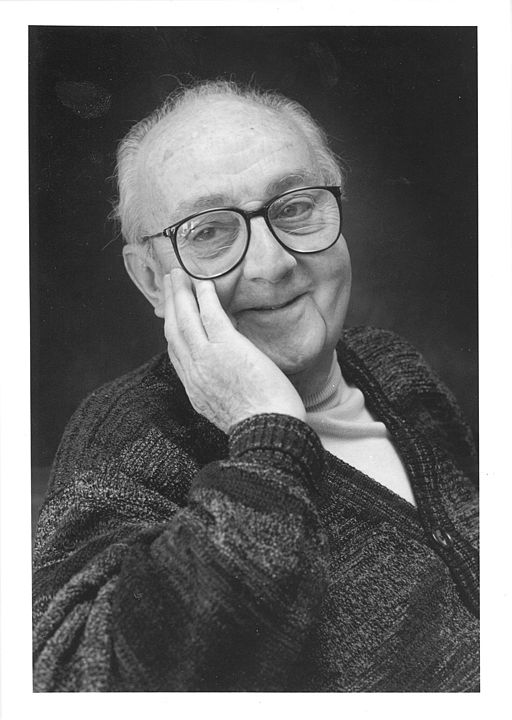
\includegraphics[width=0.9\columnwidth]{george_box.jpg}
		\end{column}
	\end{columns}
\end{frame}

\subsection{Fluxo de Trabalho Bayesiano (\textit{Workflow})\footnote{baseado em \textcite{gelmanBayesianWorkflow2020}}}
\begin{frame}{Fluxo de Trabalho Bayesiano (\textit{Workflow})\footnote{baseado em \textcite{gelmanBayesianWorkflow2020}}}
	\centering
	\begin{tikzpicture}[
			scale=0.8,
			transform shape, thick,
			every node/.style={text width=3.5cm, align=center},
			constructs/.style = {draw,
					ellipse,
					minimum width=4cm,
					minimum height=2cm}
		]
		\node[constructs] (Modelo) {Especificação do Modelo};
		\node[constructs] [right = of Modelo] (Priori) {Elicitação das \textit{Prioris}};
		\node[constructs] [right = of Priori] (Posterior) {Inferência da Posterior};
		\draw [<->, line width=1pt] (Modelo) to [out=45,in=135] node[above] {\textit{Prior Predictive Check}} (Priori);
		%\draw [->, line width=1pt] (Priori) to [out=225,in=315] {} (Modelo);
		\draw [<->, line width=1pt] (Priori) to [out=45,in=135] node[above] {\textit{Posterior Predictive Check}} (Posterior);
		%\draw [->, line width=1pt] (Posterior) to [out=225,in=315] {} (Priori);
	\end{tikzpicture}
\end{frame}

\subsection{Verificação Preditiva da \textit{Priori} (\textit{Prior Predictive Check})}
\begin{frame}{Verificação Preditiva da \textit{Priori} (\textit{Prior Predictive Check})}
	Em especial, antes de começar a alimentar o modelo com dados precisamos fazer uma
	checagem de todas as nossas \textit{prioris}.
	\vfill
	De maneira muito simples, consiste em simular parâmetros com base nas suas distribuições
	especificadas \textit{a priori} no modelo sem qualquer condicionamento aos dados e
	sem envolvimento nenhum da função de verossimilhança.
	\vfill
	Independentemente do nível de informação especificada na \textit{priori},
	é sempre importante realizar uma análise de sensibilidade prévia para entender completamente
	a influência que as \textit{prioris} têm na posterior.
\end{frame}

\begin{frame}{Verificação Preditiva da \textit{Priori} no \href{http://mc-stan.org/rstanarm/}{\texttt{rstanarm}} e \href{https://paul-buerkner.github.io/brms/}{\texttt{brms}}}
	\begin{vfilleditems}
		\item \texttt{rstanarm}: em qualquer função \text6t{stan\_*()} usar o argumento \texttt{prior\_PD = TRUE}
		\item \texttt{brms}: na função \textit{brm()} usar o argumento \texttt{sample\_prior = "only"}
	\end{vfilleditems}
\end{frame}

\subsubsection{Verificação Preditiva da \textit{Priori} no \texttt{rstanarm}}
\begin{frame}[fragile]{Verificação Preditiva da \textit{Priori} no \href{http://mc-stan.org/rstanarm/}{\texttt{rstanarm}}}
	\begin{lstlisting}
    stan_glm(y ~ ...,
        prior = normal(c(0, 0), c(5, 6)),
        prior_intercept = student_t(4, 0, 10),
        prior_aux = cauchy(0, 3),
        @prior_PD = TRUE@)
    \end{lstlisting}
\end{frame}
\subsubsection{Verificação Preditiva da \textit{Priori} no \texttt{brms}}
\begin{frame}[fragile]{Verificação Preditiva da \textit{Priori} no \href{https://paul-buerkner.github.io/brms/}{\texttt{brms}}}
	\begin{lstlisting}
    brm(y ~ x1 + x2,
        prior = c(
          prior(normal(0, 5), class = b, coef = x1),
          prior(normal(0, 6), class = b, coef = x2),
          prior(student_t(4, 0, 10), class = Intercept),
          prior(cauchy(0, 3), class = sigma)
        ),
        @sample_prior = "only"@)
    \end{lstlisting}
\end{frame}

\begin{frame}{Verificação Preditiva da \textit{Priori} no \href{https://paul-buerkner.github.io/brms/}{\texttt{brms}}}
	O interessante do \href{https://paul-buerkner.github.io/brms/}{\texttt{brms}} é
	que conseguimos naturalmente visualizar hipóteses sobre os valores do parâmetros de modelos
	estimados pela função \lstinline!brm()!
	% library(brms)
	% library(ggplot2)
	% library(ggdark)
	% library(bayesplot)
	% library(tikzDevice)
	% theme_set(dark_theme_light())
	% bayesplot_theme_set(dark_theme_light())
	% brms_custom_prior <- brm(mpg ~ wt + am, data = mtcars, chains = 1,
	%  prior = c(
	%    prior(normal(0, 5), class = b, coef = wt),
	%    prior(normal(0, 6), class = b, coef = am),
	%    prior(student_t(4, 0, 10), class = Intercept),
	%    prior(cauchy(0, 3), class = sigma)
	%  ),
	%  sample_prior = "only")
	% tikz(file = "slides/images/brms_prior_check.tex")
	% plot(hypothesis(brms_custom_prior, "Intercept = 0"))
	% dev.off()
	\begin{figure}
		\centering
		\resizebox{.35\linewidth}{!}{\input{images/brms_prior_check.tex}}
	\end{figure}
\end{frame}

\subsection{Verificação Preditiva da Posterior (\textit{Posterior Predictive Check})}
\begin{frame}{Verificação Preditiva da Posterior (\textit{Posterior Predictive Check})}
	Precisamos nos certificar que a nossa distribuição posterior de $\boldsymbol{y}$
	consegue capturar todas as nuanças da densidade real de $\boldsymbol{y}$.
	\vfill
	Isto é um procedimento chamado de Verificação Preditiva da Posterior
	(\textit{Posterior Predictive Check}) e é geralmente auferido com uma inspeção
	visual\footnote{também fazemos inspeções matemáticas probabilísticas,
		veja a seção de Comparação de Modelos} da densidade real de $\boldsymbol{y}$
	contrastada com amostragens da densidade
	posterior de $\boldsymbol{y}$ estimada pelo modelo Bayesiano.
	\vfill
	O propósito é comparar o histograma da variável dependente $\boldsymbol{y}$ contra o histograma variáveis dependentes simuladas
	pelo modelo $\boldsymbol{y}_{\text{rep}}$ após a estimação dos parâmetros. A ideia é
	que os histogramas reais e simulados se misturem e não haja divergências.
\end{frame}

\begin{frame}{Verificação Preditiva da Posterior no \href{http://mc-stan.org/rstanarm/}{\texttt{rstanarm}} e \href{https://paul-buerkner.github.io/brms/}{\texttt{brms}}}
	\begin{vfilleditems}
		\item \texttt{rstanarm}: função \lstinline!pp_check()! em qualquer modelo oriundo das funções \lstinline!stan_*()!
		\item \texttt{brms}: função \lstinline!pp_check()! em qualquer modelo oriundo da função \lstinline!brm()!
	\end{vfilleditems}
\end{frame}

\subsubsection{Verificação Preditiva da Posterior no \texttt{rstanarm}}
\begin{frame}[fragile]{Verificação Preditiva da Posterior no \href{http://mc-stan.org/rstanarm/}{\texttt{rstanarm}}}
	\begin{lstlisting}
    rstanarm_fit <- stan_glm(mpg ~ wt + am, data = mtcars)
    @pp_check(rstanarm_fit)@
    \end{lstlisting}
\end{frame}

\begin{frame}{Verificação Preditiva da Posterior no \href{http://mc-stan.org/rstanarm/}{\texttt{rstanarm}}}
	% library(rstanarm)
	% library(ggplot2)
	% library(ggdark)
	% library(bayesplot)
	% library(tikzDevice)
	% theme_set(dark_theme_light())
	% bayesplot_theme_set(dark_theme_light())
	% rstanarm_fit <- stan_glm(mpg ~ wt + am, data = mtcars)
	% tikz(file = "slides/images/pp_check_rstanarm.tex")
	% pp_check(rstanarm_fit, nreps = 10, seed = 123, type = "dens_overlay")
	% dev.off()
	\begin{columns}
		\begin{column}{0.5\textwidth}
			\begin{figure}
				\centering
				\resizebox{0.8\columnwidth}{!}{\input{images/pp_check_rstanarm.tex}}
			\end{figure}
		\end{column}
	\end{columns}
\end{frame}

\subsubsection{Verificação Preditiva da Posterior no \texttt{brms}}
\begin{frame}[fragile]{Verificação Preditiva da Posterior no \href{https://paul-buerkner.github.io/brms/}{\texttt{brms}}}
	O interessante do \href{https://paul-buerkner.github.io/brms/}{\texttt{brms}} é
	que conseguimos olhar o PPC da distribuição CDF empírica (\textit{ECDF}) também:
	\vfill
	\begin{lstlisting}
    brms_fit <- brm(mpg ~ wt + am, data = mtcars)
    @pp_check(brmsfit)@
    @pp_check(brmsfit, type = "ecdf_overlay")@
    \end{lstlisting}
\end{frame}

\begin{frame}{Verificação Preditiva da Posterior no \href{https://paul-buerkner.github.io/brms/}{\texttt{brms}}}
	% library(brms)
	% library(ggplot2)
	% library(ggdark)
	% library(bayesplot)
	% library(tikzDevice)
	% theme_set(dark_theme_light())
	% bayesplot_theme_set(dark_theme_light())
	% brms_fit <- brm(mpg ~ wt + am, data = mtcars)
	% tikz(file = "slides/images/pp_check_brms.tex")
	% pp_check(brms_fit, nreps = 10, seed = 123)
	% dev.off()
	% tikz(file = "slides/images/pp_check_brms_ecdf.tex")
	% pp_check(brms_fit, nreps = 10, seed = 123, type = "ecdf_overlay")
	% dev.off()
	\begin{columns}
		\begin{column}{0.5\textwidth}
			\begin{figure}
				\centering
				\resizebox{0.8\columnwidth}{!}{\input{images/pp_check_brms.tex}}
			\end{figure}
		\end{column}
		\begin{column}{0.5\textwidth}
			\begin{figure}
				\centering
				\resizebox{0.8\columnwidth}{!}{\input{images/pp_check_brms_ecdf.tex}}
			\end{figure}
		\end{column}
	\end{columns}
\end{frame}

\section{Regressão Linear}

\subsection{Leituras Recomendadas}
\begin{frame}{Regressão Linear - Leituras Recomendadas}
	\begin{vfilleditems}
		\item \textcite{gelman2013bayesian}:
		\begin{vfilleditems}
			\item Capítulo 14: Introduction to regression models
			\item Capítulo 16: Generalized linear models
		\end{vfilleditems}
		\item \textcite{mcelreath2020statistical} - Capítulo 4: Geocentric Models
		\item \textcite{gelman2020regression}:
		\begin{vfilleditems}
			\item Capítulo 7: Linear regression with a single predictor
			\item Capítulo 8: Fitting regression models
			\item Capítulo 10: Linear regression with multiple predictors
		\end{vfilleditems}
		\item \textcite{storopoli2021estatisticabayesianaR} - Regressão Linear
		\item Tutorial de \texttt{rstanarm} de \textcite{muth2018user}
		\item \href{http://mc-stan.org/rstanarm/articles/continuous.html}{Vinheta do \texttt{rstanarm} sobre Modelos Lineares Contínuos}
	\end{vfilleditems}
\end{frame}

\subsection{Especificação da Regressão Linear}
\begin{frame}{O que é Regressão Linear?}
	Vamos falar de um classe de modelo conhecido como regressão linear.
	A ideia aqui é modelar uma variável dependente sendo a combinação linear de
	variáveis independentes.
	$$
		\boldsymbol{y} = \alpha +  \mathbf{X} \boldsymbol{\beta} + \epsilon
	$$
	Sendo que:
	\begin{vfilleditems}
		\item $\boldsymbol{y}$ -- variável dependente
		\item $\alpha$ -- constante (também chamada de \textit{intercept})
		\item $\boldsymbol{\beta}$ -- vetor de coeficientes
		\item $\mathbf{X}$ -- matriz de dados
		\item $\epsilon$ -- erro do modelo
	\end{vfilleditems}
\end{frame}

\begin{frame}{Especificação da Regressão Linear}
	Para estimar a constante $\alpha$ e os coeficientes $\boldsymbol{\beta}$ usamos uma função de verosimilhança
	Gaussiana/normal. Matematicamente o modelo de regressão Bayesiano é:
	$$
		\begin{aligned}
			\boldsymbol{y}     & \sim \text{Normal}\left( \alpha +  \mathbf{X} \boldsymbol{\beta}, \sigma \right) \\
			\alpha             & \sim \text{Normal}(\mu_\alpha, \sigma_\alpha)                                    \\
			\boldsymbol{\beta} & \sim \text{Normal}(\mu_{\boldsymbol{\beta}}, \sigma_{\boldsymbol{\beta}})        \\
			\sigma             & \sim \text{Exponencial}(\lambda_\sigma)
		\end{aligned}
	$$
\end{frame}

\begin{frame}{Especificação da Regressão Linear}
	O que falta é especificar quais são as \textit{prioris} dos parâmetros do modelo:
	\begin{vfilleditems}
		\item Distribuição \textit{priori} de $\alpha$ -- Conhecimento que temos da constante do modelo
		\item Distribuição \textit{priori} de $\boldsymbol{\beta}$ -- Conhecimento que temos dos coeficientes das variáveis independentes do modelo
		\item Distribuição \textit{priori} de $\sigma$ -- Conhecimento que temos sobre o erro do modelo.
	\end{vfilleditems}
	\vfill
	\footnotesize
	Importante que o erro pode ser somente positivo. Além disso é intuitivo colocar uma
	distribuição que dê peso maior para valores próximos de zero, mas que permita
	também valores distantes de zero, portanto uma distribuição com cauda longa é
	bem-vinda. Distribuições candidatas são a $\text{Exponencial}$ que só tem
	suporte nos numeros reais positivos (então já resolve a questão de erros negativos)
	ou a $\text{Cauchy}^+$ truncada para apenas números positivos\footnote{lembrando
		que a distribuição Cauchy é a $t$ de Student com graus de liberdade $\nu = 1$}
\end{frame}

\begin{frame}{Especificação da Regressão Linear}
	O nosso objetivo é \textbf{encontrar a distribuição posterior dos parâmetros de
		interesse} do modelo ($\alpha$ e $\boldsymbol{\beta}$) calculando a distribuição
	posterior completa de:
	$$
		P(\boldsymbol{\theta} \mid \boldsymbol{y}) = P(\alpha, \boldsymbol{\beta}, \sigma \mid \boldsymbol{y})
	$$
\end{frame}

\subsection{Regressão Linear no \texttt{rstarnarm}}
\begin{frame}[fragile]{Regressão Linear no \href{http://mc-stan.org/rstanarm/}{\texttt{rstanarm}}}
	Usamos a função \texttt{stan\_glm()} com o argumento \texttt{family = gaussian(link = "identity")}:
	\vfill
	\begin{lstlisting}[basicstyle=\small]
    modelo_linear <- stan_glm(
    y ~ ...,
    data = df,
    family = @gaussian(link = "identity")@,
    prior = ...,
    prior_intercept = ...,
    prior_aux = ...
    )
    \end{lstlisting}
\end{frame}

\subsection{Regressão Linear no \texttt{brms}}
\begin{frame}[fragile]{Regressão Linear no \href{https://paul-buerkner.github.io/brms/}{\texttt{brms}}}
	Usamos a função \texttt{brm()} com o argumento \texttt{family = gaussian(link = "identity")}:
	\vfill
	\begin{lstlisting}[basicstyle=\small]
    modelo_linear <- brm(
    y ~ ...,
    data = df,
    family = @gaussian(link = "identity")@,
    prior = c(
        set_prior("...", class = "b", coef = "..."),
                ...
        set_prior("...", class = "b", coef = "intercept"),
        set_prior("...", class = "sigma")
        )
    )
    \end{lstlisting}
\end{frame}

\section{Regressão Logística}

\subsection{Leituras Recomendadas}
\begin{frame}{Regressão Logística - Leituras Recomendadas}
	\begin{vfilleditems}
		\item \textcite{gelman2013bayesian} - Capítulo 16: Generalized linear models
		\item \textcite{mcelreath2020statistical}:
		\begin{vfilleditems}
			\item Capítulo 10: Big Entropy and the Generalized Linear Model
			\item Capítulo 11, Seção 11.1: Binomialregression
		\end{vfilleditems}
		\item \textcite{gelman2020regression}:
		\begin{vfilleditems}
			\item Capítulo 13: Logistic regression
			\item Capítulo 14: Working with logistic regression
			\item Capítulo 15, Seção 15.3: Logistic-binomial model
			\item Capítulo 15, Seção 15.4: Probit regression
		\end{vfilleditems}
		\item \textcite{storopoli2021estatisticabayesianaR} - Regressão Logística
		\item Tutorial de \texttt{rstanarm} de \textcite{muth2018user}
		\item \href{http://mc-stan.org/rstanarm/articles/binomial.html}{Vinheta do \texttt{rstanarm} sobre Modelos Lineares Generalizados com dados Binários}
	\end{vfilleditems}
\end{frame}

\begin{frame}{Bem-Vindo ao Mundo Mágico dos Modelos Lineares Generalizados}
	Saindo do universo dos modelos lineares, começamos a nos aventurar nos modelos
	linares generalizados (\textit{generalized linear models} -- GLM).
	\vfill
	O primeiro deles é a \textbf{regressão logística}
	(também chamada de regressão binomial).
\end{frame}

\subsection{Dados Binários}
\begin{frame}{Dados Binários\footnote{também conhecido como dicotômico, \textit{dummy}, etc.}}
	Usamos regressão logística quando a nossa variável dependente é \textbf{binária}.
	Ela possui apenas dois valores distintos,
	geralmente codificados como $0$ ou $1$.
\end{frame}

\subsection{O que é Regressão Logística?}
\begin{frame}{O que é Regressão Logística?}
	Uma regressão logística se comporta exatamente como um modelo linear:
	faz uma predição simplesmente computando uma soma ponderada das variáveis
	independentes $\mathbf{X}$ pelos coeficientes estimados $\boldsymbol{\beta}$,
	mais uma constante $\alpha$. Porém ao invés de retornar um valor contínuo
	$\boldsymbol{y}$, como a regressão linear, retorna a \textbf{função logística}
	desse valor:
	$$
		\text{Logística}(x) = \frac{1}{1 + e^{-x}}
	$$
\end{frame}


\subsubsection{Função Logit}
% https://en.wikipedia.org/wiki/Logit
% padrão da family binomial(link = "logit")

\begin{frame}{Função Logística}
	\begin{tikzpicture}
		\begin{axis}[every axis plot, line width=2pt,
				ylabel={$\text{Logística}(x)$},
				xlabel={$x$},
				domain=-10:10,samples=200,
				axis x line*=bottom, % no box around the plot, only x and y axis
				axis y line*=left % the * suppresses the arrow tips
			]

			\addplot [blue] (x,{1/(1+exp(-x))});
		\end{axis}
	\end{tikzpicture}
\end{frame}

\subsubsection{Função Probit}
% https://en.wikipedia.org/wiki/Probit
\begin{frame}{Função Probit}
	Às vezes podemos também usar a \textbf{função probit} (usualmente representada
	ela letra grega $\Phi$) que é a CDF da distribuição Normal:
	$$
		\Phi (x)= \frac {1}{\sqrt {2 \pi}}\int _{-\infty }^{x}e^{-t^{2}/2}\,dt
	$$
\end{frame}

\begin{frame}{Função Probit}
	\begin{tikzpicture}
		\begin{axis}[every axis plot, line width=2pt,
				ylabel={$\Phi(x)$},
				xlabel={$x$},
				domain=-10:10,samples=200,
				axis x line*=bottom, % no box around the plot, only x and y axis
				axis y line*=left % the * suppresses the arrow tips
			]

			\addplot [blue] {normcdf(0, 1)};
		\end{axis}
	\end{tikzpicture}
\end{frame}

\subsubsection{Função Logística versus Função Probit}
\begin{frame}{Função Logística versus Função Probit}
	\begin{tikzpicture}
		\begin{axis}[every axis plot, line width=1pt,
				ylabel={$f(x)$},
				xlabel={$x$},
				domain=-10:10,samples=200,
				axis x line*=bottom, % no box around the plot, only x and y axis
				axis y line*=left % the * suppresses the arrow tips
			]
			\addplot [blue] (x,{1/(1+exp(-x))});
			\addlegendentry{Logística}
			\addplot [red] {normcdf(0, 1)};
			\addlegendentry{Probit}
		\end{axis}
	\end{tikzpicture}
\end{frame}

\subsection{Comparativo com a Regressão Linear}
\begin{frame}{Comparativo com a Regressão Linear}
	A regressão linear segue a seguinte formulação matemática:
	\small
	$$
		\text{Linear} = \alpha + \beta_1 x_1 + \beta_2 x_2 + \dots + \beta_k x_k
	$$
	Onde:
	\begin{vfilleditems}
		\item \small $\alpha$ - constante
		\item \small $\boldsymbol{\beta} = \beta_1, \beta_2, \dots, \beta_k$ - coeficientes das variáveis independentes $x_1, x_2, \dots, x_k$
		\item \small $k$ - número de variáveis independentes
	\end{vfilleditems}
	Se você implementar uma pequena gambiarra matemática, você terá a \textbf{regressão logística}:
	\begin{vfilleditems}
		\item \small $\hat{p} = \text{Logística}(\text{Linear}) = \frac{1}{1 + e^{-\operatorname{Linear}}}$ - probabilidade prevista da observação ser o valor $1$
		\item \small $\hat{y} = \begin{cases} 0 & \text { se } \hat{p} < 0.5 \\ 1 & \text { se } \hat{p} \geq 0.5 \end{cases}$ - previsão do valor discreto de $\boldsymbol{y}$
	\end{vfilleditems}
\end{frame}

\subsection{Especificação da Regressão Logística}
\begin{frame}{Especificação da Regressão Logística}
	Podemos modelar regressão logística de duas maneiras:
	\begin{vfilleditems}
		\item com a \textbf{verossimilhança Bernoulli} modelamos uma variável dependente
		\textbf{binária} $\boldsymbol{y}$ que é o resultado de um experimento de
		Bernoulli com uma certa probabilidade $p$.
		\item com a \textbf{verossimilhança binomial} modelamos uma variável dependente
		\textbf{contínua} $\boldsymbol{y}$ que é o número de sucessos de $n$
		experimentos Bernoulli independentes.
	\end{vfilleditems}
\end{frame}

\subsubsection{Verossimilhança Bernoulli}
\begin{frame}{Verossimilhança Bernoulli}
	\small
	$$
		\begin{aligned}
			\boldsymbol{y}     & \sim \text{Bernoulli}\left( p\right)                                      \\
			p                  & \sim \text{Logística/Logit}(\alpha +  \mathbf{X} \boldsymbol{\beta})      \\
			\alpha             & \sim \text{Normal}(\mu_\alpha, \sigma_\alpha)                             \\
			\boldsymbol{\beta} & \sim \text{Normal}(\mu_{\boldsymbol{\beta}}, \sigma_{\boldsymbol{\beta}})
		\end{aligned}
	$$
	Sendo que:
	\begin{vfilleditems}
		\item \small $\boldsymbol{y}$ - \textbf{variável dependente binária}
		\item \small $p$ - probabilidade de $\boldsymbol{y}$ tomar o valor de $\boldsymbol{y}$ - sucesso de um experimento Bernoulli independente
		\item \small $\text{Logística/Logit}$ - função logística ou logit
		\item \small $\alpha$ - constante (também chamada de \textit{intercept})
		\item \small $\boldsymbol{\beta}$ - vetor de coeficientes
		\item \small $\mathbf{X}$ - matriz de dados
	\end{vfilleditems}
\end{frame}

\subsubsection{Verossimilhança Binomial}
\begin{frame}{Verossimilhança Binomial}
	\small
	$$
		\begin{aligned}
			\boldsymbol{y}     & \sim \text{Binomial}\left(n,  p\right)                                    \\
			p                  & \sim \text{Logística/Probit}(\alpha +  \mathbf{X} \boldsymbol{\beta})     \\
			\alpha             & \sim \text{Normal}(\mu_\alpha, \sigma_\alpha)                             \\
			\boldsymbol{\beta} & \sim \text{Normal}(\mu_{\boldsymbol{\beta}}, \sigma_{\boldsymbol{\beta}})
		\end{aligned}
	$$
	Sendo que:
	\begin{vfilleditems}
		\item \small $\boldsymbol{y}$ - \textbf{variável dependente contínua} - sucessos de $n$ experimentos Bernoulli independentes
		\item \small $n$ - número de experimentos Bernoulli independentes
		\item \small $p$ - probabilidade de $\boldsymbol{y}$ tomar o valor de $\boldsymbol{y}$ - sucesso de um experimento Bernoulli independente
		\item \small $\text{Logística/Logit}$ - função logística ou logit
		\item \small $\alpha$ - constante (também chamada de \textit{intercept})
		\item \small $\boldsymbol{\beta}$ - vetor de coeficientes
		\item \small $\mathbf{X}$ - matriz de dados
	\end{vfilleditems}
\end{frame}

\begin{frame}{Especificação da Regressão Logística}
	O nosso objetivo é \textbf{encontrar a distribuição posterior dos parâmetros de
		interesse} do modelo ($\alpha$ e $\boldsymbol{\beta}$) calculando a distribuição
	posterior completa de:
	$$
		P(\boldsymbol{\theta} \mid \boldsymbol{y}) = P(\alpha, \boldsymbol{\beta} \mid \boldsymbol{y})
	$$
\end{frame}

\subsection{Intepretação dos Coeficientes}
\begin{frame}{Interpretação dos Coeficientes}
	Ao vermos a fórmula de regressão logística percebemos a interpretação dos
	coeficientes requer uma transformação. A transformação que precisamos fazer á a
	que inverte a função logística.
\end{frame}
\begin{frame}{Probabilidade versus Chances\footnote{em inglês \textit{probability} e
			\textit{odds}}}
	\small
	Mas antes preciso falar sobre\textbf{qual a diferença matemática
		entre probabilidade e chances}.
	\begin{vfilleditems}
		\item \small \textbf{Probabilidade}: um número real entre $0$ e $1$ que
		representa a certeza de que um evento irá acontecer por meio de frequências
		de longo-prazo (probabilidade frequentista) ou níveis de credibilidade
		(probabilidade Bayesiana).
		\item \small Chances é um número positivo real ($\mathbb{R}^+$) que mensura
		também a certeza de um evento. Mas essa certeza não é expressa como uma
		probabilidade (algo entre $0$ e $1$), mas como uma \textbf{razão entre a
			quantidade de resultados que produzem o evento desejado e a quantidade de
			resultados que \textit{não} produzem o evento desejado}:
		$$
			\text{Chances} = \frac{p}{1-p}
		$$
		onde $p$ é a probabilidade.
	\end{vfilleditems}
\end{frame}

\begin{frame}{Probabilidade versus Chances}
	$$
		\text{Chances} = \frac{p}{1-p}
	$$
	onde $p$ é a probabilidade.
	\vfill
	\begin{vfilleditems}
		\item Chance com o valor de $1$ é uma chance neutra
		algo como uma moeda justa $p = \frac{1}{2}$
		\item Chances abaixo de $1$ decrescem a probabilidade de vermos um
		certo evento
		\item Chances acima de $1$ aumentam a probabilidade do evento.
	\end{vfilleditems}
\end{frame}

\begin{frame}{Log das Chances\footnote{em inglês \textit{logodds}}}
	Se você revisitar a função logística, verá que ela tanto a constante quanto
	os coeficientes de $\boldsymbol{\beta}$ são literalmente o log da
	chance:
	$$
		\begin{aligned}
			p                  & \sim \text{Logística/Logit}(\alpha +  \mathbf{X} \boldsymbol{\beta} )                        \\
			p                  & \sim \text{Logística/Logit}(\alpha) + \text{Logística/Logit}( \mathbf{X} \boldsymbol{\beta}) \\
			\boldsymbol{\beta} & = \frac{1}{1 + e^{(-\boldsymbol{\beta})}}                                                    \\
			\boldsymbol{\beta} & = \log(\text{Chance})
		\end{aligned}
	$$
\end{frame}

\begin{frame}{Log das Chances}
	Portanto, os coeficientes de uma regressão logística são expressados em
	\textit{logodds} no qual $0$ é o elemento neutro e qualquer número acima ou
	abaixo aumenta ou diminui as chances de obtermos um "sucesso"~de
	$\boldsymbol{y}$. Para termos uma interpretação mais intuitiva
	(igual a das casas de apostas) precisamos converter as \textit{logodds}
	em chances revertendo a função $\log$. Para isso basta "exponenciar"~os
	valores de $\alpha$ e $\boldsymbol{\beta}$:
	$$
		\begin{aligned}
			\text{Chances}(\alpha)               & = e^\alpha               \\
			\text{Chances}({\boldsymbol{\beta}}) & = e^{\boldsymbol{\beta}}
		\end{aligned}
	$$
\end{frame}

\subsection{Regressão Logística no \texttt{rstarnarm}}
\begin{frame}[fragile]{Regressão Logística no \href{http://mc-stan.org/rstanarm/}{\texttt{rstanarm}}}
	Usamos a função \texttt{stan\_glm()} com os argumentos \texttt{family = binomial(link = "logit")} ou
	\texttt{family = binomial(link = "probit")}:
	\vfill
	\begin{lstlisting}[basicstyle=\small]
    modelo_binomial <- stan_glm(
    y ~ ...,
    data = df,
    family = @binomial(link = "logit")@, # ou link = "probit"
    prior = ...,
    prior_intercept = ...
    )
    \end{lstlisting}
\end{frame}

\subsection{Regressão Logística no \texttt{brms}}
\begin{frame}[fragile]{Regressão Logística no \href{https://paul-buerkner.github.io/brms/}{\texttt{brms}}}
	Usamos a função \texttt{brm()} com os argumentos \texttt{family = binomial(link = "logit")} ou
	\texttt{family = binomial(link = "probit")}:
	\vfill
	\begin{lstlisting}[basicstyle=\small]
    modelo_binomial <- brm(
    y ~ ...,
    data = df,
    family = @binomial(link = "logit")@, # ou link = "probit"
    prior = c(
        set_prior("...", class = "b", coef = "..."),
                ...
        set_prior("...", class = "b", coef = "intercept")
        )
    )
    \end{lstlisting}
\end{frame}

\section{Regressão de Poisson}

\subsection{Leituras Recomendadas}
\begin{frame}{Regressão de Poisson - Leituras Recomendadas}
    \begin{vfilleditems}
        \item \textcite{gelman2013bayesian} - Capítulo 16: Generalized linear models
        \item \textcite{mcelreath2020statistical}:
        \begin{vfilleditems}
            \item Capítulo 10: Big Entropy and the Generalized Linear Model
            \item Capítulo 11, Seção 11.2: Poisson regression
        \end{vfilleditems}
        \item \textcite{gelman2020regression} - Capítulo 15, Seção 15.2: Poisson and negative binomial regression
        \item \textcite{storopoli2021estatisticabayesianaR} - Regressão de Poisson
        \item Tutorial de \texttt{rstanarm} de \textcite{muth2018user}
        \item \href{http://mc-stan.org/rstanarm/articles/count.html}{Vinheta do \texttt{rstanarm} sobre Modelos Lineares Generalizados com dados de Contagem}
    \end{vfilleditems}
\end{frame}

\begin{frame}{Bem-Vindo ao Mundo Mágico dos Modelos Lineares Generalizados}
    Saindo do universo dos modelos lineares, começamos a nos aventurar nos modelos
    linares generalizados (\textit{generalized linear models} -- GLM).
    \vfill
    O segundo deles é a \textbf{regressão de Poisson}.
\end{frame}

\subsection{Dados de Contagem\footnote{\textit{count data}}}
\begin{frame}{Dados de Contagem}
    Regressão de Poisson é usada quando a nossa variável dependente só pode
    tomar \textbf{valores positivos}, geralmente em contextos de
    \textbf{dados de contagem}.
\end{frame}

\subsection{O que é Regressão de Poisson?}
\begin{frame}{O que é Regressão de Poisson?}
    Uma regressão de Poisson se comporta exatamente como um modelo linear:
    faz uma predição simplesmente computando uma soma ponderada das variáveis
    independentes $\mathbf{X}$ pelos coeficientes estimados $\boldsymbol{\beta}$,
    $\boldsymbol{y}$, como a regressão linear, retorna o \textbf{logarítmo natural}
    desse valor:
    $$
    \log(\boldsymbol{y})= \alpha \cdot \beta_1 x_1 \cdot \beta_2 x_2 \cdot \ldots \cdot \beta_k x_k
    $$
    que é o mesmo que:
    $$
    \boldsymbol{y} = e^{(\alpha + \beta_1 x_1 + \beta_2 x_2 + \ldots + \beta_k x_k)}
    $$
\end{frame}

\subsubsection{Função Exponencial}
\begin{frame}{Função Exponencial}
    A função $e^x$ é chamada de função exponencial:
    \begin{tikzpicture}
        \begin{axis}[every axis plot, line width=2pt,
            ylabel={$e^x$},
            xlabel={$x$},
            domain=-5:10,samples=200,
            axis x line*=bottom, % no box around the plot, only x and y axis
            axis y line*=left % the * suppresses the arrow tips
            ]

            \addplot [blue] (x,{exp(x))});
        \end{axis}
    \end{tikzpicture}
\end{frame}

\subsection{Comparativo com a Regressão Linear}
\begin{frame}{Comparativo com a Regressão Linear}
    A regressão linear segue a seguinte formulação matemática:
    \small
    $$
    \text{Linear} = \alpha + \beta_1 x_1 + \beta_2 x_2 + \ldots + \beta_k x_k
    $$
    Onde:
    \begin{vfilleditems}
        \item \small $\alpha$ - constante
        \item \small $\boldsymbol{\beta} = \beta_1, \beta_2, \dots, \beta_k$ - coeficientes das variáveis independentes $x_1, x_2, \dots, x_k$
        \item \small $k$ - número de variáveis independentes
    \end{vfilleditems}
    Se você implementar uma pequena gambiarra matemática, você terá a \textbf{regressão de Poisson}:
    \begin{vfilleditems}
        \item \small $\log{y} = e^{\text{Linear}} = e^{\alpha + \beta_1 x_1 + \beta_2 x_2 + \ldots + \beta_k x_k}$
    \end{vfilleditems}
\end{frame}

\subsection{Especificação da Regressão de Poisson}
\begin{frame}{Especificação da Regressão de Poisson}
    Podemos fazer uma regressão de Poisson se a variável dependente
    $\boldsymbol{y}$ for uma variável com dados de contagem, ou seja,
    $\boldsymbol{y}$ somente toma valores positivos. A função de \textbf{verossimilhança de
    Poisson} usa uma constante $\alpha$ e os coeficientes $\boldsymbol{\beta}$
    porém estes são "exponenciados"~($e^x$):
    $$
    \begin{aligned}
    \boldsymbol{y} &\sim \text{Poisson}\left( e^{(\alpha +  \mathbf{X} \boldsymbol{\beta})} \right) \\
    \alpha &\sim \text{Normal}(\mu_\alpha, \sigma_\alpha) \\
    \boldsymbol{\beta} &\sim \text{Normal}(\mu_{\boldsymbol{\beta}}, \sigma_{\boldsymbol{\beta}})
    \end{aligned}
    $$
\end{frame}

\subsection{Intepretação dos Coeficientes}
\begin{frame}{Interpretação dos Coeficientes}
    Ao vermos a fórmula de regressão de Poisson percebemos a interpretação dos
    coeficientes requer uma transformação. A transformação que precisamos fazer á a
    que inverte a função logarítmica:
    $$
    \log^{-1}(x) = e^x
    $$
    Então precisamos novamente "exponenciar"~os valores de $\alpha$ e
    $\boldsymbol{\beta}$:
    $$
    \begin{aligned}
        \boldsymbol{y} &= e^{(\alpha +  \mathbf{X} \boldsymbol{\beta})} \\
        &= e^{\alpha} \cdot e^{ \left( X_{(1)} \cdot \beta_{(1)} \right) } \cdot e^{ \left( X_{(2)} \cdot \beta_{(2)} \right) } \cdot \dots \cdot e^{ \left( X_{(k)} \cdot \beta_{(k)} \right) }
    \end{aligned}
    $$
\end{frame}

\subsection{Regressão de Poisson no \texttt{rstarnarm}}
\begin{frame}[fragile]{Regressão de Poisson no \href{http://mc-stan.org/rstanarm/}{\texttt{rstanarm}}}
    Usamos a função \texttt{stan\_glm()} com o argumento \texttt{poisson(link = "log")}:
    \vfill
    \begin{lstlisting}[basicstyle=\small]
    modelo_poisson <- stan_glm(
    y ~ ...,
    data = df,
    family = @poisson(link = "log")@,
    prior = ...,
    prior_intercept = ...
    )
    \end{lstlisting}
\end{frame}

\subsection{Regressão de Poisson no \texttt{brms}}
\begin{frame}[fragile]{Regressão de Poisson no \href{https://paul-buerkner.github.io/brms/}{\texttt{brms}}}
    Usamos a função \texttt{brm()} com o argumento \texttt{poisson(link = "log")}:
    \vfill
    \begin{lstlisting}[basicstyle=\small]
    modelo_poisson <- brm(
    y ~ ...,
    data = df,
    family = @poisson(link = "log")@,
    prior = c(
        set_prior("...", class = "b", coef = "..."),
                ...
        set_prior("...", class = "b", coef = "intercept")
        )
    )
    \end{lstlisting}
\end{frame}

\section{Regressão Robusta}

\subsection{Leituras Recomendadas}
\begin{frame}{Regressão Robusta - Leituras Recomendadas}
	\begin{vfilleditems}
		\item \textcite{gelman2013bayesian} - Capítulo 17: Models for robust inference
		\item \textcite{mcelreath2020statistical} - Capítulo 12: Monsters and Mixtures
		\item \textcite{gelman2020regression}:
		\begin{vfilleditems}
			\item Capítulo 15, Seção 15.6: Robust regression using the t model
			\item Capítulo 15, Seção 15.8: Going beyond generalized linear models
		\end{vfilleditems}
		\item \textcite{storopoli2021estatisticabayesianaR} - Regressão Robusta
		\item Tutorial de \texttt{brms} de \textcite{burknerAdvancedBayesianMultilevel2018}
	\end{vfilleditems}
\end{frame}

\begin{frame}{Modelos Robustos\footnote{\href{https://github.com/allisonhorst/stats-illustrations}{digura de Allison Horst (CC-BY-4.0)}}}
	\begin{columns}
		\begin{column}{0.6\textwidth}
			Quase sempre nossos dados no mundo real são bem estranhos.
			\vfill
			Por conveniência usamos modelos simples. Mas sempre se
			pergunte. De que maneiras a inferência da posterior depende de:
			\vfill
			\begin{vfilleditems}
				\item Observações extremas (\textit{outliers})?
				\item Suposições de modelo não-acessíveis?
			\end{vfilleditems}
			\vfill
			Além disso vamos usar \textbf{exclusivamente} o
			\href{https://paul-buerkner.github.io/brms/}{\texttt{brms}}
			ao invés do \href{http://mc-stan.org/rstanarm/}{\texttt{rstanarm}}.
		\end{column}
		\begin{column}{0.4\textwidth}
			\includegraphics[width=0.9\columnwidth]{not_normal_transparent.png}
		\end{column}
	\end{columns}
\end{frame}

\subsection{Dados com \textit{Outliers}}
\begin{frame}{Dados com \textit{Outliers}}
	Modelos baseados na \textbf{distribuição normal são notoriamente "não robustos"}~
	para outliers, no sentido de que \textbf{uma única observação \textit{outlier} pode
		afetar fortemente a inferência para todos os parâmetros no modelo},
	mesmo aqueles com pouca conexão substantiva com a observação \textit{outlier}.
\end{frame}

\subsection{Superdispersão}
\begin{frame}{Superdispersão (\textit{Overdispersion})}
	\begin{defn}[Superdispersão e Subdispersão]
		A superdispersão \textit{overdispersion} e a subdispersão\footnote{bem
			mais raro no mundo real}
		\textit{underdispersion} referem-se a dados que mostram mais ou menos
		variação do que o esperado com base em um modelo de probabilidade.
		\parencite{gelman2020regression}
	\end{defn}
	\vfill
	Para cada um dos modelos padrão, há de fato uma \textbf{extensão natural} em que um
	\textbf{único} parâmetro é adicionado para permitir a superdispersão
	\parencite{gelman2013bayesian}.
\end{frame}

\begin{frame}{Exemplo de Superdispersão}
	\begin{exemplo}[Acidentes de Trânsito]
		Suponha que você esteja analisando acidentes de trânsito.
		O modelo usualmente usado nesses tipos de fenômenos é a \textbf{Regressão
			de Poisson}.
		A distribuição de Poisson possui o mesmo valor como média e variância.
		Então, se você encontrar uma variação nos dados maior que a verossimilhança Poisson
		permite, o modelo probabilístico provavelmente não conseguirá reproduzir com
		fidelidade o fenômeno modelado.
	\end{exemplo}
\end{frame}

\subsection{Versões com Superdispersão dos Modelos Probabilísticos Padrões}
\subsubsection{$t$ de Student ao invés da Normal}
\begin{frame}{$t$ de Student ao invés da Normal}
	A distribuição $t$ de Student tem uma \textbf{cauda mais longa} que a
	distribuição Normal.
	\vfill
	O que faz uma boa candidata para \textbf{acomodar observações \textit{outliers} sem
		gerar instabilidades na inferência dos parâmetros}.
	\vfill
	Do ponto de vista Bayesiano, não há nada especial na verossimilhança
	Gaussiana/Normal. É apenas uma distribuição probabilística especificada
	em um modelo. Podemos deixar o modelo mais robusto ao usarmos uma distribuição $t$
	de Student como função de verossimilhança.
\end{frame}

\begin{frame}{$t$ de Student ao invés da Normal}
	\centering
	\begin{tikzpicture}
		\begin{axis}[every axis plot, line width=2pt,
				ylabel=PDF,
				domain=-4:4,samples=200,
				axis x line*=bottom, % no box around the plot, only x and y axis
				axis y line*=left % the * suppresses the arrow tips
			]

			\addplot [blue] {gaussian(0, 1)};
			\addlegendentry{Normal}
			\addplot [red] {student(3)};
			\addlegendentry{Student com $\nu=3$}
		\end{axis}
	\end{tikzpicture}
\end{frame}

\begin{frame}{$t$ de Student ao invés da Normal}
	Ao usarmos uma verossimilhança $t$ de Student ao invés da Normal, o erro do modelo,
	$\sigma$ não segue uma distribuição normal, mas sim uma distribuição $t$ de Student:
	$$
		\begin{aligned}
			\boldsymbol{y}     & \sim \text{Student}\left( \nu, \alpha + \mathbf{X} \boldsymbol{\beta}, \sigma \right) \\
			\alpha             & \sim \text{Normal}(\mu_\alpha, \sigma_\alpha)                                         \\
			\boldsymbol{\beta} & \sim \text{Normal}(\mu_{\boldsymbol{\beta}}, \sigma_{\boldsymbol{\beta}})             \\
			\nu                & \sim \text{Log-Normal}(2, 1)                                                          \\
			\sigma             & \sim \text{Exponencial}(\lambda_\sigma)
		\end{aligned}
	$$
	\small
	Além disso, é apropriado incluir os graus de liberdade $\nu$ como um parâmetro a
	ser estimado pelo modelo \parencite{gelman2013bayesian}. Uma \textit{priori}
	de cauda longa e restrita a somente tomar valores positivos é adequada.
\end{frame}

\begin{frame}[fragile]{\href{https://paul-buerkner.github.io/brms/}{\texttt{brms}} -- $t$ de Student ao invés da Normal}
	\begin{lstlisting}
    brm(...
      family = @student(link = "identity")@
    )
    \end{lstlisting}
\end{frame}

\subsubsection{Beta-Binomial ao invés da Binomial}
\begin{frame}{Beta-Binomial ao invés da Binomial}
	A distribuição binomial tem uma limitação prática de que temos somente um
	parâmetro livre\footnote{já que $n$ vem dos dados} ($p$), o que implica em
	a \textbf{variância ser determinada pela média}. Isso faz com que a verossimilhança
	binomial \textbf{não} seja robusta à superdispersão.
	\vfill
	Uma alternativa robusta é a \textbf{distribuição beta-binomial}, que, como o nome
	sugere, é uma \textbf{mistura beta de binomiais}. Além disso, permite com que
	a \textbf{variância seja diferente da média}, garantindo \textbf{robustez}
	à superdispersão.
\end{frame}

\begin{frame}{Beta-Binomial ao invés da Binomial}
	A distribuição beta-binomial é uma binomial, mas a probabilidade $p$ é parametrizada
	com uma distribuição $\text{Beta}(\alpha, \beta)$. Geralmente usamos $\alpha$ como
	a probabilidade $p$ da binomial e $\beta$ (também usado às vezes $\phi$) é o parâmetro adicional para controlar
	superdispersão. Valores de $\beta$/$\phi$ iguais a $1$ fazem a beta-binomial se comportar
	igual a uma binomial.
	$$
		\begin{aligned}
			\boldsymbol{y}     & \sim \text{Beta-Binomial}(n, p, \phi)                                     \\
			p                  & \sim \text{Logística/Probit}(\alpha +  \mathbf{X} \boldsymbol{\beta})     \\
			\alpha             & \sim \text{Normal}(\mu_\alpha, \sigma_\alpha)                             \\
			\boldsymbol{\beta} & \sim \text{Normal}(\mu_{\boldsymbol{\beta}}, \sigma_{\boldsymbol{\beta}}) \\
			\phi               & \sim \text{Exponencial}(1)
		\end{aligned}
	$$
	\small
	É apropriado incluir o parâmetro de superdispersão $\beta$ como um parâmetro a
	ser estimado pelo modelo \parencite{gelman2013bayesian,mcelreath2020statistical}.
	Uma \textit{priori} de cauda longa e restrita a somente tomar valores positivos é
	adequada.
\end{frame}

\begin{frame}[fragile]{\href{https://paul-buerkner.github.io/brms/}{\texttt{brms}} -- Beta-Binomial ao invés da Binomial\footnote{sugiro verem \href{https://bookdown.org/content/4857/monsters-and-mixtures.html}{essa implementação Solomon Kurz}}}
	\begin{lstlisting}[basicstyle=\footnotesize]
# verossimilhanca customizada
beta_binomial2 <- @custom_family@("beta_binomial2",
  dpars = c("mu", "phi"),
  links = c("logit", "log"), lb = c(NA, 0),
  type = "int", vars = "vint1[n]")
stan_funs <- "
  real beta_binomial2_lpmf(int y, real mu, real phi, int T) {
    return beta_binomial_lpmf(y | T, mu * phi, (1 - mu) * phi);
  }
  int beta_binomial2_rng(real mu, real phi, int T) {
    return beta_binomial_rng(T, mu * phi, (1 - mu) * phi);
  }"
stanvars <- stanvar(scode = stan_funs, block = "functions")
brm(...,
  family = @beta_binomial2@,  # verossimilhanca customizada
  prior = c(..., @prior(exponential(1), class = phi@))
    \end{lstlisting}
\end{frame}

\subsubsection{$t$ de Student ao invés da Binomial}
\begin{frame}{$t$ de Student ao invés da Binomial}
	\small
	Também chamada de \textit{Robit}\footnote{há uma bela discussão com Gelman,
		Vehtari e Kurz no
		\href{https://discourse.mc-stan.org/t/robit-regression-not-robust/21245/}{
			\textit{discourse} do \texttt{Stan}}} \parencite{gelman2013bayesian, gelman2020regression}.
	A ideia é "robustizar"~ a regressão logística com uma formulação usando dados
	latentes $z$ e dar uma uma distribução $t$ de Student aos erros latentes $\epsilon$:
	$$
		\begin{aligned}
			y_i        & = \begin{cases} 0 & \text{se } z_i < 0 \\ 1 & \text{se }\ z_i > 0 \end{cases} \\
			z_i        & = X_i \boldsymbol{\beta} + \epsilon_i                                         \\
			\epsilon_i & \sim \text{Student} \left (\nu, 0, \sqrt{\frac{\nu - 2}{\nu}} \right)         \\
			\nu        & \sim \text{Gamma}(2, 0.1) \in \left[2, \infty \right)
		\end{aligned}
	$$
	\footnotesize
	O grande segredo aqui é usar uma distribuição Gamma como \textit{priori}
	dos graus de liberdade $\nu$ truncada para valor mínimo de $\nu = 2$. Outra opção
	é literalmente especificar $\nu=4$.
\end{frame}

\begin{frame}[fragile]{\href{https://paul-buerkner.github.io/brms/}{\texttt{brms}} -- $t$ de Student ao invés da Binomial}
	\begin{lstlisting}[basicstyle=\footnotesize]
stan_inv_robit <- "
real inv_robit(real y, real nu) {
    return(student_t_cdf(y, nu, 0, sqrt((nu - 2) / nu)));
    }"
stanvar_inv_robit <- stanvar(scode = stan_inv_robit, block = "functions")
robit_formula <-
bf(y_c | trials(1) ~ inv_robit(eta, nu),
    nlf(eta ~ b0 + b1 * x),
    b0 + b1 ~ 1,
    nu ~ 1,
    nl = TRUE)
brm(formula = robit_formula,
    family = @binomial("identity")@,
    formula = robit_formula,
    prior = c(prior(normal(0, 1), nlpar = b0),
    prior(normal(0, 1), nlpar = b1),
    prior(gamma(2, 0.1), nlpar = nu, @lb = 2@)),
    stanvars = stanvar_inv_robit)
    \end{lstlisting}
\end{frame}

\subsubsection{Binomial Negativa ao invés de Poisson}
\begin{frame}{Binomial Negativa ao invés de Poisson}
	Esse é o exemplo que falamos sobre superdispersão.
	A distribuição de Poisson possui o mesmo valor como média e variância.
	\vfill
	Então, se você encontrar superdispersão, provavelmente precisará de uma alternativa
	robusta à Poisson. Aqui que entra a binomial negativa que "robustiza"~
	a Poisson com um parâmetro extra $\phi$.
	\vfill
	Esse parâmetro é a probabilidade de sucessos $p$ da distribuição binomial negativa
	e geralmente usamos uma distribuição gamma como \textit{priori} para que $\phi$
	cumpra a função de um parâmetro de~"dispersão recíproca".
\end{frame}

\begin{frame}{Binomial Negativa ao invés de Poisson}
	$$
		\begin{aligned}
			\boldsymbol{y}     & \sim \text{Binomial Negativa} \left( e^{(\alpha + \mathbf{X} \boldsymbol{\beta})}, \phi \right) \\
			\phi               & \sim \text{Gamma}(0.01, 0.01)                                                                   \\
			\alpha             & \sim \text{Normal}(\mu_\alpha, \sigma_\alpha)                                                   \\
			\boldsymbol{\beta} & \sim \text{Normal}(\mu_{\boldsymbol{\beta}}, \sigma_{\boldsymbol{\beta}})
		\end{aligned}
	$$
	A ideia é dar uma \textit{priori} cauda longa para $\phi$, algo como
	$\text{Gamma}(0.01, 0.01)$ funciona.
\end{frame}

\begin{frame}[fragile]{\href{https://paul-buerkner.github.io/brms/}{\texttt{brms}} -- Binomial Negativa ao invés de Poisson}
	\begin{lstlisting}
    brm(...
      family = @negbinomial(link = "log")@
    )
    \end{lstlisting}
\end{frame}

\subsubsection{Mistura de Binomial Negativa ao invés de Poisson}
\begin{frame}{Mistura de Binomial Negativa ao invés de Poisson}
	\small
	Mesmo usando uma binomial negativa, caso a superdispersão seja muito acentuada,
	em especial quando temos muita \textbf{inflação de zeros} (\textit{zero-inflated}),
	o seu modelo ainda pode resultar em patologias.
	Uma outra sugestão é usar uma mistura de binomial negativa \parencite{mcelreath2020statistical}.
	Aqui, $S_i$ é uma variável binária (\textit{dummy})
	indicando se a observação $i$ tem valor diferente de zero ou não.
	$S_i$ pode ser modelado usando uma regressão logística:
	$$
		\begin{aligned}
			\boldsymbol{y}
			                    & \begin{cases}
				                      = 0,                                                                                             & \text{ se } S_i = 0 \\
				                      \sim \text{Binomial Negativa} \left( e^{(\alpha + \mathbf{X} \boldsymbol{\beta})}, \phi \right), & \text{ se } S_i = 1
			                      \end{cases} \\
			P(S_i = 1)          & = \text{Logística/Logit}(\mathbf{X} \boldsymbol{\gamma})                                                               \\
			\boldsymbol{\gamma} & \sim \text{Beta}(1, 1)
		\end{aligned}
	$$
	\small
	$\boldsymbol{\gamma}$ é um novo conjunto de coeficientes para essa parte do modelo com
	\textit{prioris} uniformes de $\text{Beta} (1, 1)$.
\end{frame}

\begin{frame}[fragile]{\href{https://paul-buerkner.github.io/brms/}{\texttt{brms}} -- Mistura de Binomial Negativa ao invés de Poisson}
	\begin{lstlisting}
    brm(...
      family = @zero_inflated_negbinomial(link = "log")@,
      prior = c(
          ...
        @prior(gamma(0.01, 0.01), class = shape)@,
        @prior(beta(1, 1), class = zi)@
    ))
    \end{lstlisting}
\end{frame}

\subsection{Por quê usar Modelos Não-Robustos?}
\begin{frame}{Por quê usar Modelos Não-Robustos?}
	O \textbf{teorema do limite central} nos diz que a distribuição \textbf{normal}
	é uma modelo apropriado para dados que são formados como a \textbf{soma de um grande número
		de componentes independentes}.
	\vfill
	Mesmo quando não estão naturalmente implícitos na estrutura de um problema,
	os \textbf{modelos simples não-robustos são computacionalmente convenientes}.
	\vfill
	Claro o que deve sempre guiar a sua escolha de modelo, além da natureza específica
	do processo de geração de dados do fenômeno que você está estudando, é
	a \textbf{verificação preditiva da posterior}.
\end{frame}

\section{Modelos Multiníveis}

\subsection{Leituras Recomendadas}
\begin{frame}{Modelos Multiníveis - Leituras Recomendadas}
    \begin{vfilleditems}
        \item \textcite{gelman2013bayesian}:
        \begin{vfilleditems}
            \item Capítulo 5: Hierarchical models
            \item Capítulo 15: Hierarchical linear models
        \end{vfilleditems}
        \item \textcite{mcelreath2020statistical}:
        \begin{vfilleditems}
            \item Capítulo 13: Models With Memory
            \item Capítulo 14: Adventures in Covariance
        \end{vfilleditems}
        \item \textcite{storopoli2021estatisticabayesianaR} - Modelos Multiníveis
        \item Tutorial de \texttt{rstanarm} de \textcite{muth2018user}
        \item Tutorial de \texttt{brms} de \textcite{burknerAdvancedBayesianMultilevel2018}
        \item \textcite{gelmanDataAnalysisUsing2007}
        \item Estudo de caso do Michael Betancourt sobre \href{https://betanalpha.github.io/assets/case_studies/hierarchical_modeling.html}{Modelos Hierárquicos}
        \item \textcite{kruschke2015bayesian}
    \end{vfilleditems}
\end{frame}

\subsection{O que são Modelos Multiníveis?}
\begin{frame}{\textit{I have many names...}}
    Modelos multiníveis também são conhecidos por vários nomes\footnote{para uma listagem completa \href{https://statmodeling.stat.columbia.edu/2019/09/18/all-the-names-for-hierarchical-and-multilevel-modeling/}{veja aqui}}:
    \begin{vfilleditems}
        \item Modelos Hierárquicos (\textit{Hierarchical Models})
        \item Modelos de Efeitos Aleatórios (\textit{Random Effects Models})
        \item Modelos de Efeitos Mistos (\textit{Mixed Effects Models})
        \item Modelos de Dados em Painel (\textit{Cross-Sectional Models})
        \item Modelos de Dados Aninhados (\textit{Nested Data Models})
    \end{vfilleditems}
\end{frame}

\begin{frame}{O que são Modelos Multiníveis?}
    \begin{defn}[Modelos Multiníveis]
        Modelo estatístico escrito em níveis \textit{múltiplos} (forma hierárquica)
        que estima os parâmetros da distribuição posterior usando a abordagem
        Bayesiana. Os submodelos se combinam para formar o modelo hierárquico, e o
        teorema de Bayes é usado para integrá-los aos dados observados e contabilizar
        toda a incerteza que está presente.
    \end{defn}
    \vfill
    Os modelos hierárquicos são descrições matemáticas que envolvem vários parâmetros,
    de modo que as estimativas de alguns parâmetros dependem significativamente
    dos valores de outros parâmetros.
\end{frame}

\begin{frame}{O que são Modelos Multiníveis?}
    \small
    Hiperparamêtro $\phi$ que parametriza os parâmetros $\theta_1, \theta_2, \dots, \theta_K$
    que por fim são usados para inferir a densidade posterior de alguma variável de interesse
    $\mathbf{y} = y_1, y_2, \dots, y_K$
    \begin{adjustbox}{max width=1.0\textwidth}
    \begin{tikzpicture}[scale=0.3, thick]

        \pgfmathsetmacro{\r}{2}
        \pgfmathsetmacro{\dx}{0}
        \pgfmathsetmacro{\dy}{0}

        \draw[black] (-21 + \dx, -7 + \dy) rectangle (21 + \dx, 13 + \dy);

        \filldraw[fill=dark, draw=dark, line width=1.5] (-12 + \dx, 9 + \dy) circle (\r)
        node[color=white] { $y_{1}$ };

        \filldraw[fill=dark, draw=dark, line width=1.5] (-6 + \dx, 9 + \dy) circle (\r)
        node[color=white] { $\ldots$ };

        \filldraw[fill=dark, draw=dark, line width=1.5] (0 + \dx, 9 + \dy) circle (\r)
        node[color=white] { $y_{k}$ };

        \filldraw[fill=dark, draw=dark, line width=1.5] (6 + \dx, 9 + \dy) circle (\r)
        node[color=white] { $\ldots$ };

        \filldraw[fill=dark, draw=dark, line width=1.5] (12 + \dx, 9 + \dy) circle (\r)
        node[color=white] { $y_{K}$ };

        \draw[->, >=stealth, color=mid, line width=1.5] (-12 + \dx, 3 + \r + \dy) -- (-12 + \dx, 9 - \r + \dy);
        \draw[->, >=stealth, color=mid, line width=1.5] (-6 + \dx, 3 + \r + \dy) -- (-6 + \dx, 9 - \r + \dy);
        \draw[->, >=stealth, color=mid, line width=1.5] (0 + \dx, 3 + \r + \dy) -- (0 + \dx, 9 - \r + \dy);
        \draw[->, >=stealth, color=mid, line width=1.5] (6 + \dx, 3 + \r + \dy) -- (6 + \dx, 9 - \r + \dy);
        \draw[->, >=stealth, color=mid, line width=1.5] (12 + \dx, 3 + \r + \dy) -- (12 + \dx, 9 - \r + \dy);

        \filldraw[fill=black, draw=dark, line width=1.5] (-12 + \dx, 3 + \dy) circle (\r)
        node[color=white] { $\theta_{1}$ };

        \filldraw[fill=black, draw=dark, line width=1.5] (-6 + \dx, 3 + \dy) circle (\r)
        node[color=white] { $\ldots$ };

        \filldraw[fill=black, draw=dark, line width=1.5] (0 + \dx, 3 + \dy) circle (\r)
        node[color=white] { $\theta_{k}$ };

        \filldraw[fill=black, draw=dark, line width=1.5] (6 + \dx, 3 + \dy) circle (\r)
        node[color=white] { $\ldots$ };

        \filldraw[fill=black, draw=dark, line width=1.5] (12 + \dx, 3 + \dy) circle (\r)
        node[color=white] { $\theta_{K}$ };

        \draw[->, >=stealth, color=mid, line width=1.5] (0 + \dx, -3 + \r + \dy) -- (-12 + \dx, 3 - \r + \dy);
        \draw[->, >=stealth, color=mid, line width=1.5] (0 + \dx, -3 + \r + \dy) -- (-6 + \dx, 3 - \r + \dy);
        \draw[->, >=stealth, color=mid, line width=1.5] (0 + \dx, -3 + \r + \dy) -- (0 + \dx, 3 - \r + \dy);
        \draw[->, >=stealth, color=mid, line width=1.5] (0 + \dx, -3 + \r + \dy) -- (6 + \dx, 3 - \r + \dy);
        \draw[->, >=stealth, color=mid, line width=1.5] (0 + \dx, -3 + \r + \dy) -- (12 + \dx, 3 - \r + \dy);

        \filldraw[fill=black, draw=dark, line width=1.5] (0 + \dx, -3 + \dy) circle (\r)
        node[color=white] { $\phi$ };

    \end{tikzpicture}
    \end{adjustbox}
\end{frame}

\begin{frame}{O que são Modelos Multiníveis?}
    \footnotesize
    Mesmo que as observações informem diretamente apenas um único conjunto de
    parâmetros, o modelo hierárquico acopla os parâmetros individuais e fornece uma
    porta dos fundos para que as observações informem todos os contextos.
    \begin{adjustbox}{max width=1.0\textwidth}
    \begin{tikzpicture}[scale=0.3, thick]

        % Right
        \pgfmathsetmacro{\r}{2}

        \pgfmathsetmacro{\dx}{0}
        \pgfmathsetmacro{\dy}{0}

        \draw[black] (-17 + \dx, -7 + \dy) rectangle (17 + \dx, 13 + \dy);

        \fill[fill=dark, line width=1.5, opacity=0.50] (-12 + \dx, 9 + \dy) circle (\r)
        node[color=white] { $y_{1}$ };

        \fill[fill=dark, line width=1.5, opacity=0.50] (-6 + \dx, 9 + \dy) circle (\r)
        node[color=white] { $\ldots$ };

        \filldraw[fill=dark, draw=dark, line width=1.5] (0 + \dx, 9 + \dy) circle (\r)
        node[color=white] { $y_{k}$ };

        \fill[fill=dark, line width=1.5, opacity=0.50] (6 + \dx, 9 + \dy) circle (\r)
        node[color=white] { $\ldots$ };

        \fill[fill=dark, line width=1.5, opacity=0.50] (12 + \dx, 9 + \dy) circle (\r)
        node[color=white] { $y_{K}$ };

        \draw[<-, >=stealth, color=dark, line width=1.5] (0 + \dx, 3 + \r + \dy) -- (0 + \dx, 9 - \r + \dy);

        \filldraw[fill=black, draw=dark, line width=1.5] (-12 + \dx, 3 + \dy) circle (\r)
        node[color=white] { $\theta_{1}$ };

        \filldraw[fill=black, draw=dark, line width=1.5,] (-6 + \dx, 3 + \dy) circle (\r)
        node[color=white] { $\ldots$ };

        \filldraw[fill=black, draw=dark, line width=1.5] (0 + \dx, 3 + \dy) circle (\r)
        node[color=white] { $\theta_{k}$ };

        \filldraw[fill=black, draw=dark, line width=1.5] (6 + \dx, 3 + \dy) circle (\r)
        node[color=white] { $\ldots$ };

        \filldraw[fill=black, draw=dark, line width=1.5] (12 + \dx, 3 + \dy) circle (\r)
        node[color=white] { $\theta_{K}$ };

        \draw[->, >=stealth, color=dark, line width=1.5] (0 + \dx, -3 + \r + \dy) -- (-12 + \dx, 3 - \r + \dy);
        \draw[->, >=stealth, color=dark, line width=1.5] (0 + \dx, -3 + \r + \dy) -- (-6 + \dx, 3 - \r + \dy);
        \draw[<-, >=stealth, color=dark, line width=1.5] (0 + \dx, -3 + \r + \dy) -- (0 + \dx, 3 - \r + \dy);
        \draw[->, >=stealth, color=dark, line width=1.5] (0 + \dx, -3 + \r + \dy) -- (6 + \dx, 3 - \r + \dy);
        \draw[->, >=stealth, color=dark, line width=1.5] (0 + \dx, -3 + \r + \dy) -- (12 + \dx, 3 - \r + \dy);

        \filldraw[fill=black, draw=dark, line width=1.5] (0 + \dx, -3 + \dy) circle (\r)
        node[color=white] { $\phi$ };

        % Left
        \pgfmathsetmacro{\dx}{35}
        \pgfmathsetmacro{\dy}{0}

        \draw[black] (-17 + \dx, -7 + \dy) rectangle (17 + \dx, 13 + \dy);

        \filldraw[fill=dark,  draw=dark, line width=1.5] (-12 + \dx, 9 + \dy) circle (\r)
        node[color=white] { $y_{1}$ };

        \filldraw[fill=dark,  draw=dark, line width=1.5] (-6 + \dx, 9 + \dy) circle (\r)
        node[color=white] { $\ldots$ };

        \fill[fill=dark, line width=1.5, opacity=0.50] (0 + \dx, 9 + \dy) circle (\r)
        node[color=white] { $y_{k}$ };

        \filldraw[fill=dark, draw=dark, line width=1.5] (6 + \dx, 9 + \dy) circle (\r)
        node[color=white] { $\ldots$ };

        \filldraw[fill=dark, draw=dark, line width=1.5] (12 + \dx, 9 + \dy) circle (\r)
        node[color=white] { $y_{K}$ };

        \draw[<-, >=stealth, color=dark, line width=1.5] (-12 + \dx, 3 + \r + \dy) -- (-12 + \dx, 9 - \r + \dy);
        \draw[<-, >=stealth, color=dark, line width=1.5] (-6 + \dx, 3 + \r + \dy) -- (-6 + \dx, 9 - \r + \dy);
        \draw[<-, >=stealth, color=dark, line width=1.5] (6 + \dx, 3 + \r + \dy) -- (6 + \dx, 9 - \r + \dy);
        \draw[<-, >=stealth, color=dark, line width=1.5] (12 + \dx, 3 + \r + \dy) -- (12 + \dx, 9 - \r + \dy);

        \filldraw[fill=black, draw=dark, line width=1.5] (-12 + \dx, 3 + \dy) circle (\r)
        node[color=white] { $\theta_{1}$ };

        \filldraw[fill=black, draw=dark, line width=1.5,] (-6 + \dx, 3 + \dy) circle (\r)
        node[color=white] { $\ldots$ };

        \filldraw[fill=black, draw=dark, line width=1.5] (0 + \dx, 3 + \dy) circle (\r)
        node[color=white] { $\theta_{k}$ };

        \filldraw[fill=black, draw=dark, line width=1.5] (6 + \dx, 3 + \dy) circle (\r)
        node[color=white] { $\ldots$ };

        \filldraw[fill=black, draw=dark, line width=1.5] (12 + \dx, 3 + \dy) circle (\r)
        node[color=white] { $\theta_{K}$ };

        \draw[<-, >=stealth, color=dark, line width=1.5] (-\r + \dx, -3 + \dy) -- (-12 + \dx, 3 - \r + \dy);
        \draw[<-, >=stealth, color=dark, line width=1.5] ({-0.25 - \r * cos(45) + \dx}, {-3 + \r * cos(45) + \dy}) -- (-6 + \dx, 3 - \r + \dy);
        \draw[->, >=stealth, color=dark, line width=1.5] (0 + \dx, -3 + \r + \dy) -- (0 + \dx, 3 - \r + \dy);
        \draw[<-, >=stealth, color=dark, line width=1.5] ({0.25 + \r * cos(45) + \dx}, {-3 + \r * cos(45) + \dy}) -- (6 + \dx, 3 - \r + \dy);
        \draw[<-, >=stealth, color=dark, line width=1.5] (\r + \dx, -3 + \dy) -- (12 + \dx, 3 - \r + \dy);

        \filldraw[fill=black, draw=dark, line width=1.5] (0 + \dx, -3 + \dy) circle (\r)
        node[color=white] { $\phi$ };
        \end{tikzpicture}
        \end{adjustbox}

    \footnotesize
    Por exemplo, as observações do $k$-ésimo contexto, $y_k$, informam diretamente
    os parâmetros que quantificam o comportamento desse contexto, $\theta_k$.
    Esses parâmetros, entretanto, informam diretamente os parâmetros populacionais
    $\phi$ que então informam todos os outros contextos por meio do modelo hierárquico.
    Da mesma forma, as observações que informam diretamente os outros contextos
    informam indiretamente os parâmetros populacionais que então retroalimentam o $k$-ésimo
    contexto.
\end{frame}

\begin{frame}{O que são Modelos Multiníveis?}
    A \textbf{modelagem hierárquica} é usada quando as informações estão disponíveis em
    vários \textbf{níveis diferentes de unidades de} observação. A forma hierárquica de
    análise e organização auxilia no entendimento de \textbf{problemas multiparâmetros} e
    também desempenha um papel importante no desenvolvimento de \textbf{estratégias
    computacionais}.
\end{frame}

\subsection{Quando usar Modelos Multiníveis?}
\begin{frame}{Quando usar Modelos Multiníveis?}
    Modelos multiníveis são particularmente apropriados para projetos de pesquisa
    onde os dados dos participantes são organizados em mais de um nível
    (ou seja, dados aninhados -- \textit{nested data}).
    As unidades de análise geralmente são indivíduos (em um nível inferior)
    que estão aninhados em unidades contextuais/agregadas (em um nível superior).
    \vfill
    \small
    Um exemplo é quando estamos mensurando desempenho de indivíduos e temos
    informações adicionais sobre pertencimento à grupos distintos como:
    \begin{vfilleditems}
        \item \small sexo
        \item \small faixa etária
        \item \small nível hierárquico
        \item \small nível educacional
        \item \small estado/província de residência
    \end{vfilleditems}
\end{frame}

\begin{frame}{Quando usar Modelos Multiníveis?}
    O mais importante é que \textbf{não seja violado} o \textbf{princípio da permutabilidade}
    \parencite{definettiTheoryProbability1974}.
    \vfill
    Esse pressuposto parte do princípio que os \textbf{grupos são permutáveis}.
\end{frame}

\begin{frame}{Revisitando a Permutabilidade \parencite{definettiTheoryProbability1974}\footnote{figuras adaptadas de \href{https://betanalpha.github.io/assets/case_studies/hierarchical_modeling.html}{Michael Betancourt (CC-BY-SA-4.0)}}}
    \begin{adjustbox}{max width=1.0\textwidth}
        \begin{tikzpicture}[scale=0.3, thick]

        % Left
        \begin{scope}[shift={(-36, 0)}]

        \draw[white] (-17, 0) rectangle (17, 15);

        \fill[dark] (-10, 4) circle (1);
        \begin{scope}
          \clip (-10, 4) circle (1);
          \draw[color=light, line width=5, rotate=30] (-5.25, 8.25) arc[x radius=1.4, y radius=0.2, start angle=0, end angle=-180];
        \end{scope}
        \node at (-10, 10) {\includegraphics[width=2cm]{cup_up.png}};

        \fill[mid] (0, 4) circle (1);
        \begin{scope}
          \clip (0, 4) circle (1);
          \draw[color=dark, line width=2] (1.1, 4.3) arc[x radius=1.1, y radius=0.2, start angle=0, end angle=180];
          \draw[color=dark, line width=2] (1.1, 3.7) arc[x radius=1.1, y radius=0.2, start angle=0, end angle=180];
        \end{scope}
        \node at (0, 10) {\includegraphics[width=2cm]{cup_up.png}};

        \fill[dark] (+10, 4) circle (1);
        \begin{scope}
          \clip (10, 4) circle (1);
          \draw[color=mid, line width=1] (10, 3) -- (10, 5);
          \draw[color=mid, line width=1] (10.25, 5) arc[x radius=0.3, y radius=1.1, start angle=90, end angle=-90];
          \draw[color=mid, line width=1] (9.75, 5) arc[x radius=0.3, y radius=1.1, start angle=90, end angle=270];
        \end{scope}
        \node at (+10, 10) {\includegraphics[width=2cm]{cup_up.png}};

        \end{scope}

        % Right
        \begin{scope}[shift={(0, 0)}]

        \draw[white] (-17, 0) rectangle (17, 15);

        \fill[dark] (-10, 4) circle (1);
        \node at (-10, 7) {\includegraphics[width=2cm]{cup_down.png}};
        \begin{scope}[scale=0.7, shift={(-17, 3)}, rotate=-5]
            \fill[dark, rounded corners=3] (0, 0) rectangle (10, 6);
            \fill[black] (0, 0.5) rectangle (10, 3.5);
            \node[text=white, align=center, rotate=-5] at (5, 5.2) { \small \textsf{OLÁ} };
            \node[text=white, align=center, rotate=-5] at (5, 4.1) { \tiny \textsf{meu nome é } };
            \node[text=white, align=center, rotate=0] at (5.25, 2) { \large \textsl{Grupo 1} };
          \end{scope}

        \fill[dark] (0, 4) circle (1);
        \node at (0, 7) {\includegraphics[width=2cm]{cup_down.png}};
        \begin{scope}[scale=0.7, shift={(-2, 3)}, rotate=10]
            \fill[dark, rounded corners=3] (0, 0) rectangle (10, 6);
            \fill[black] (0, 0.5) rectangle (10, 3.5);
            \node[text=white, align=center, rotate=10] at (5, 5.2) { \small \textsf{OLÁ} };
            \node[text=white, align=center, rotate=10] at (5, 4.1) { \tiny \textsf{meu nome é } };
            \node[text=white, align=center, rotate=7] at (5.25, 2) { \large \textsl{Grupo 2} };
          \end{scope}

        \fill[dark] (+10, 4) circle (1);
        \node at (+10, 7) {\includegraphics[width=2cm]{cup_down.png}};
        \begin{scope}[scale=0.7, shift={(12, 3)}, rotate=1]
            \fill[dark, rounded corners=3] (0, 0) rectangle (10, 6);
            \fill[black] (0, 0.5) rectangle (10, 3.5);
            \node[text=white, align=center, rotate=1] at (5, 5.2) { \small \textsf{OLÁ} };
            \node[text=white, align=center, rotate=1] at (5, 4.1) { \tiny \textsf{meu nome é } };
            \node[text=white, align=center, rotate=1] at (5.25, 2) { \large \textsl{Grupo 3} };
          \end{scope}
        \end{scope}
        \end{tikzpicture}
    \end{adjustbox}
\end{frame}

\begin{frame}{Revisitando a Permutabilidade \parencite{definettiTheoryProbability1974}\footnote{figuras adaptadas de \href{https://betanalpha.github.io/assets/case_studies/hierarchical_modeling.html}{Michael Betancourt (CC-BY-SA-4.0)}}}
    \begin{adjustbox}{max width=1.0\textwidth}
        \begin{tikzpicture}[scale=0.3, thick]


            \draw[white] (-17, -3) rectangle (17, 15);

            \fill[dark] (-10, 4) circle (1);
            \node at (-10, 7) {\includegraphics[width=2cm]{cup_down.png}};

            % Left
            \begin{scope}[scale=0.7, shift={(-17, 3)}, rotate=-5]
              \fill[dark, rounded corners=3] (0, 0) rectangle (10, 6);
              \fill[black] (0, 0.5) rectangle (10, 3.5);
              \node[text=white, align=center, rotate=-5] at (5, 5.2) { \small \textsf{OLÁ} };
              \node[text=white, align=center, rotate=-5] at (5, 4.1) { \tiny \textsf{meu nome é } };
              \node[text=white, align=center, rotate=0] at (5.25, 2) { \large \textsl{Grupo 1} };
            \end{scope}

            \fill[dark] (0, 4) circle (1);
            \node at (0, 7) {\includegraphics[width=2cm]{cup_down.png}};

            \begin{scope}[scale=0.7, shift={(-2, 3)}, rotate=10]
              \fill[dark, rounded corners=3] (0, 0) rectangle (10, 6);
              \fill[black] (0, 0.5) rectangle (10, 3.5);
              \node[text=white, align=center, rotate=10] at (5, 5.2) { \small \textsf{OLÁ} };
              \node[text=white, align=center, rotate=10] at (5, 4.1) { \tiny \textsf{meu nome é } };
              \node[text=white, align=center, rotate=7] at (5.25, 2) { \large \textsl{Grupo 2} };
            \end{scope}

            \fill[dark] (+10, 4) circle (1);
            \node at (+10, 7) {\includegraphics[width=2cm]{cup_down.png}};

            \begin{scope}[scale=0.7, shift={(12, 3)}, rotate=1]
              \fill[dark, rounded corners=3] (0, 0) rectangle (10, 6);
              \fill[black] (0, 0.5) rectangle (10, 3.5);
              \node[text=white, align=center, rotate=1] at (5, 5.2) { \small \textsf{OLÁ} };
              \node[text=white, align=center, rotate=1] at (5, 4.1) { \tiny \textsf{meu nome é } };
              \node[text=white, align=center, rotate=1] at (5.25, 2) { \large \textsl{Grupo 3} };
            \end{scope}

            \pgfmathsetmacro{\r}{10}
            \pgfmathsetmacro{\start}{160}
            \pgfmathsetmacro{\stop}{20}

            \draw[dark, <->, >=stealth] ({0 + \r * cos(\start)}, {8 + \r * sin(\start)})
                            arc[x radius = \r, y radius = 3, start angle=\start, end angle= \stop];

            \pgfmathsetmacro{\r}{3}
            \pgfmathsetmacro{\start}{160}
            \pgfmathsetmacro{\stop}{20}

            \draw[dark, <->, >=stealth] ({-5 + \r * cos(\start)}, {10 + \r * sin(\start)})
                            arc[x radius = \r, y radius = 0.75, start angle=\start, end angle= \stop];

            \draw[dark, <->, >=stealth] ({5 + \r * cos(\start)}, {10 + \r * sin(\start)})
                            arc[x radius = \r, y radius = 0.75, start angle=\start, end angle= \stop];

            % Right
            \begin{scope}[shift={(36, 0)}]

            \draw[white] (-17, -3) rectangle (17, 15);

            \fill[dark] (-10, 4) circle (1);
            \node at (-10, 7) {\includegraphics[width=2cm]{cup_down.png}};

            \begin{scope}[scale=0.7, shift={(-17, 3)}, rotate=-5]
              \fill[dark, rounded corners=3] (0, 0) rectangle (10, 6);
              \fill[black] (0, 0.5) rectangle (10, 3.5);
              \node[text=white, align=center, rotate=-5] at (5, 5.2) { \small \textsf{OLÁ} };
              \node[text=white, align=center, rotate=-5] at (5, 4.1) { \tiny \textsf{meu nome é } };
              \node[text=white, align=center, rotate=0] at (5.25, 2) { \large \textsl{Grupo 3} };
            \end{scope}

            \fill[dark] (0, 4) circle (1);
            \node at (0, 7) {\includegraphics[width=2cm]{cup_down.png}};

            \begin{scope}[scale=0.7, shift={(-2, 3)}, rotate=10]
              \fill[dark, rounded corners=3] (0, 0) rectangle (10, 6);
              \fill[black] (0, 0.5) rectangle (10, 3.5);
              \node[text=white, align=center, rotate=10] at (5, 5.2) { \small \textsf{OLÁ} };
              \node[text=white, align=center, rotate=10] at (5, 4.1) { \tiny \textsf{meu nome é } };
              \node[text=white, align=center, rotate=7] at (5.25, 2) { \large \textsl{Grupo 1} };
            \end{scope}

            \fill[dark] (+10, 4) circle (1);
            \node at (+10, 7) {\includegraphics[width=2cm]{cup_down.png}};

            \begin{scope}[scale=0.7, shift={(12, 3)}, rotate=1]
              \fill[dark, rounded corners=3] (0, 0) rectangle (10, 6);
              \fill[black] (0, 0.5) rectangle (10, 3.5);
              \node[text=white, align=center, rotate=1] at (5, 5.2) { \small \textsf{OLÁ} };
              \node[text=white, align=center, rotate=1] at (5, 4.1) { \tiny \textsf{meu nome é } };
              \node[text=white, align=center, rotate=1] at (5.25, 2) { \large \textsl{Grupo 2} };
            \end{scope}

            \draw[light, <->, >=stealth, line width=4]
              (-8, 6.5) .. controls (-7, 7.5) and (-6.5, 8.25) ..
              (-4.5, 8.5) .. controls (-2.5, 8.75) and (-1, 8.5) .. (0, 7);
            \draw[dark, <->, >=stealth, line width=2]
              (-7.85, 6.65) .. controls (-7, 7.5) and (-6.5, 8.25) ..
              (-4.5, 8.5) .. controls (-2.5, 8.75) and (-1, 8.5) .. (-0.15, 7.15);

            \draw[light, <->, >=stealth, line width=4]
              (3, 7.5) .. controls (4, 9) and (6.25, 9.75) ..
              (8.25, 9.5) .. controls (10.25, 9.25) and (11, 8.75) .. (12, 6.75);
            \draw[dark, <->, >=stealth, line width=2]
              (3.15, 7.65) .. controls (4, 9) and (6.25, 9.75) ..
              (8.25, 9.5) .. controls (10.25, 9.25) and (11, 8.75) .. (11.9, 6.9);

            \draw[light, <->, >=stealth, line width=4]
              (-8, 1.5) .. controls (-7, -1.5) and (2, -1.25) ..
              (4, -1) .. controls (6, -0.75) and (11, -0.5) .. (12, 1.5);
            \draw[dark, <->, >=stealth, line width=2]
              (-7.925, 1.25) .. controls (-7, -1.5) and (2, -1.25) ..
              (4, -1) .. controls (6, -0.75) and (11, -0.5) .. (11.9, 1.3);

            \end{scope}

            \end{tikzpicture}
    \end{adjustbox}
\end{frame}

\subsection{\textit{Hiperpriori} (\textit{Hyperprior})}
\begin{frame}{\textit{Hiperpriori} (\textit{Hyperprior})}
    Em modelos multiníveis temos a figura da \textit{hiperpriori}, que é
    justamente uma \textit{priori} de uma \textit{priori}:
    $$
    \begin{aligned}
        \boldsymbol{y} &\sim \text{Normal}(10, \boldsymbol{\theta}) \\
        \boldsymbol{\theta} &\sim \text{Normal}(0, \phi) \\
        \phi &\sim \text{Exponencial(1)}
    \end{aligned}
    $$
    Aqui $\boldsymbol{y}$ são variáveis de interesse que pertencem à certos
    grupos distintos. $\boldsymbol{\theta}$, uma \textit{priori} de $\boldsymbol{y}$,
    é um vetor de parâmetros de grupos com uma \textit{priori} (que se torna \textit{hyperiori})
    $\phi$.
\end{frame}

\subsection{Abordagem Frequentista versus Abordagem Bayesiana}
\begin{frame}{Abordagem Frequentista versus Abordagem Bayesiana}
  Existem modelos multíveis também na estatística frequentista.
  Todos esses estão disponíveis no pacote \texttt{lme4} \parencite{lme4}.
  \begin{vfilleditems}
    \item \textbf{otimização da função de verossimilhança} versus \textbf{aproximação da posterior via MCMC}.
    Quase sempre isso gera falha de convergência para modelos que não sejam extremamente
    simples.
    \item \textbf{modelos multiníveis frequentista não computam $p$-valores dos efeitos de grupo}\footnote{veja a explicação \href{https://stat.ethz.ch/pipermail/r-help/2006-May/094765.html}{aqui do Douglas Bates autor do pacote \texttt{lme4}}}.
    or conta da contorção matemática de diversas aproximações que a estatística
    frequentista tem que fazer o cálculo de $p$-valores de efeitos de
    grupo possuem fortes pressupostos. O principal é que os grupos são balanceados.
    Ou seja, os grupos são homogêneos no seu tamanho.
    Qualquer desbalanço na composição dos grupos (um grupo com mais observações que outros) resulta em
    $p$-valores patológicos e que não podem ser confiáveis.
  \end{vfilleditems}
\end{frame}

\begin{frame}{Abordagem Frequentista versus Abordagem Bayesiana}
  Sumarizando, a abordagem \textbf{frequentista para modelos multiníveis não é robusta}
  tanto no processo da \textbf{inferência} (\textbf{falhas de convergência}
  da estimação de máxima verossimilhança), quanto nos \textbf{resultados} dessa
  inferência (não computa $p$-valores por conta de \textbf{fortes pressupostos
  que quase sempre são violados}).
\end{frame}

\subsection{3 Abordagens de Modelos Multiníveis}

\begin{frame}{3 Abordagens de Modelos Multiníveis}
  \begin{vfilleditems}
    \item \textit{Random-intercept model}: Modelo no qual cada grupo recebe uma
    constante (\textit{intercept}) diferente além da constante global e coeficientes
    globais
    \item \textit{Random-slope model}: Modelo no qual cada grupo recebe um coeficiente
    (\textit{slope}) diferente para cada variável independente além da constante global
    \item \textit{Random-intercept-slope model}: Modelo no qual cada grupo recebe tanto
    uma constante (\textit{intercept}) quanto um coeficiente (\textit{slope})
    diferente para cada variável independente além da constante global
  \end{vfilleditems}
  \small
  \texttt{rstanarm} e \texttt{brms} possuem as funcionalidades completas para rodar
  modelos multiníveis e a única coisa a se fazer é alterar a fórmula. Para
  \texttt{rstanarm}, há uma segunda mudança também que não usamos mais a função
  \texttt{stan\_glm()} mas sim a função \texttt{stan\_glmer()}. Para \texttt{brms}
  não há mudança e usamos a mesma função \texttt{brm()}.
\end{frame}

\subsubsection{\textit{Random-intercept model}}
\begin{frame}[fragile]{\textit{Random-intercept model}}
  A primeira abordagem é o \textit{random-intercept model} na qual especificamos
  para cada grupo uma constante diferente, além da constante global. Essas constantes
  são amostradas de uma \textit{hiperpriori}.
  \vfill
  A fórmula a ser usada segue este padrão:
  \begin{lstlisting}
    y ~ (1 | group) + x1 + x2
  \end{lstlisting}
  \vfill
  O \texttt{(1 | group)} na fórmula sinaliza que a constante \texttt{1}
  deve ser também especificada para cada um dos grupos listados nos valores
  da variável \texttt{group}.
\end{frame}

\begin{frame}[fragile]{\textit{Random-intercept model}}
  Caso queira remover do modelo a constante global\footnote{algo que eu recomendo
  apenas se tiver \textbf{muita fundamentação teórica} para tal manobra}
  é só especificar o \texttt{0} como constante global. Isto sinaliza que o modelo
  possui apenas constantes para cada grupo e que não há uma constante global a
  ser estimada:
  \begin{lstlisting}
    y ~ 0 + (1 | group) + x1 + x2
  \end{lstlisting}
  \vfill
  Além disso você pode especificar uma constante para quantos grupos quiser.
  É só adicioná-los na fórmula:
  \begin{lstlisting}
  y ~ (1 | group1) + (1 | group2) + x1 + x2
  \end{lstlisting}
\end{frame}

\begin{frame}{Especificações Matemáticas dos Modelos Multiníveis}
  Os modelos hierárquicos geralmente são especificados assim.
  \vfill
  Temos $N$ observações organizadas em $J$ grupos com $K$ variáveis independentes.
  \vfill
  O truque aqui é que inserimos uma coluna de $1$ na matrix de dados $\mathbf{X}$.
  Matematicamente isto se comporta como se esta coluna fosse uma variável de identidade
  (pois o número $1$ na operação de multiplicação $1 \cdot \beta$ é o elemento identidade.
  Ele mapeia $x \to x$ mantendo o valor de $x$) e, consequentemente, podemos interpretar o
  coeficiente dessa coluna como a constante do modelo\footnote{por isso que nas fórmulas do
  \texttt{R} o \texttt{1} é interpretado como a constante do modelo. Substitua-o por uma coluna
  de $0$ de temos um modelo sem constante, por isso o \texttt{0} nas fórmulas é interpretado
  como um modelo ausente de constante}.
\end{frame}

\begin{frame}{Especificações Matemáticas dos Modelos Multiníveis}
  Então temos os dados como uma matriz:
  $$
  \mathbf{X} =
  \begin{bmatrix}
  1 & x_{11} & x_{12} & \cdots & x_{1K} \\
  1 & x_{21} & x_{22} & \cdots & x_{2K} \\
  \vdots & \cdots & \cdots & \ddots & \vdots \\
  1 & x_{N1} & x_{N2} & \cdots & x_{NK}
  \end{bmatrix}
  $$
\end{frame}

\begin{frame}{Especificação Matemática -- \textit{Random-intercept model}}
  Matematicamente o \textit{Random-intercept model} para uma regressão linear é:
  $$
  \begin{aligned}
  \mathbf{y} &\sim \text{Normal}\left( \alpha + \alpha_j + \mathbf{X} \cdot \boldsymbol{\beta}, \sigma \right) \\
  \alpha &\sim \text{Normal}(\mu_\alpha, \sigma_\alpha) \\
  \alpha_j &\sim \text{Normal}(0, \tau) \\
  \boldsymbol{\beta} &\sim \text{Normal}(\mu_{\boldsymbol{\beta}}, \sigma_{\boldsymbol{\beta}}) \\
  \tau &\sim \text{Cauchy}^+(0, \psi_{\alpha})\\
  \sigma &\sim \text{Exponential}(\lambda_\sigma)
  \end{aligned}
  $$
\end{frame}

\subsubsection{\textit{Random-slope model}}
\begin{frame}[fragile]{\textit{Random-slope model}}
  A segunda abordagem é o \textit{random-slope model} na qual especificamos para cada
  grupo um coeficiente diferente para cada variável independente desejada,
  além da constante global. Esses coeficientes são amostrados de uma \textit{hiperpriori}.
  \vfill
  A fórmula a ser usada segue este padrão:
  \begin{lstlisting}
    y ~ (0 + x1 | group) + (0 + x2 | group)
  \end{lstlisting}
  \vfill
  Note que usamos o \texttt{0} pois neste caso sinalizamos que apenas a variável
  independente deve possuir coeficientes para cada grupo e não a constante.
\end{frame}

\begin{frame}{Especificação Matemática -- \textit{Random-slope model}}
  Matematicamente o \textit{Random-slope model} para uma regressão linear é:
  $$
  \begin{aligned}
    \boldsymbol{y} &\sim \text{Normal}(\alpha + \mathbf{X} \boldsymbol{\beta}_{j}, \sigma) \\
    \boldsymbol{\beta}_j &\sim \text{Normal Multivariada}(\boldsymbol{\mu}_j, \boldsymbol{\Sigma})
    \quad \text{para}\quad j \in \{ 1, \dots, J \} \\
    \boldsymbol{\Sigma} &\sim \text{LKJ}(\eta) \\
    \alpha &\sim \text{Normal}(\mu_\alpha, \sigma_\alpha) \\
    \sigma &\sim \text{Exponencial}(\lambda_\sigma)
  \end{aligned}
  $$
  Cada vetor de coeficientes $\boldsymbol{\beta}_j$ representa os coeficientes
  das colunas de $\mathbf{X}$ para cada grupo $j \in J$.
\end{frame}

\begin{frame}{Especificação Matemática -- \textit{Random-slope model}}
  Caso queira mais grupos é só adicioná-los ao modelo como $J_1, J_2, \dots$:
  $$
  \begin{aligned}
  \boldsymbol{y} &\sim \text{Normal}(\alpha + \mathbf{X} \boldsymbol{\beta}_{j1} + \mathbf{X} \boldsymbol{\beta}_{j2}, \sigma) \\
  \boldsymbol{\beta}_{j1} &\sim \text{Normal Multivariada}(\boldsymbol{\mu}_{j1}, \boldsymbol{\Sigma}_1)
  \quad \text{para}\quad j_1 \in \{ 1, \dots, J_1 \} \\
  \boldsymbol{\beta}_{j2} &\sim \text{Normal Multivariada}(\boldsymbol{\mu}_{j2}, \boldsymbol{\Sigma}_2)
  \quad \text{para}\quad j_2 \in \{ 1, \dots, J_2 \} \\
  \boldsymbol{\Sigma}_1 &\sim \text{LKJ}(\eta_1) \\
  \boldsymbol{\Sigma}_2 &\sim \text{LKJ}(\eta_2) \\
  \alpha &\sim \text{Normal}(\mu_\alpha, \sigma_\alpha) \\
  \sigma &\sim \text{Exponencial}(\lambda_\sigma)
  \end{aligned}
  $$
\end{frame}

\begin{frame}{\textit{Prioris} para Matrizes de Covariância}
  Podemos especificar uma \textit{priori} para a matriz de covariância
  $\boldsymbol{\Sigma}$.
  \vfill
  Para eficiência computacional podemos fazer a matriz de covariância
  $\boldsymbol{\Sigma}$ vire uma matriz de correlação. Toda matriz de
  covariância pode ser decomposta em:
  $$
  \boldsymbol{\Sigma}=\text{diag}_\text{matrix}(\boldsymbol{\tau}) \cdot \boldsymbol{\Omega} \cdot \text{diag}_\text{matrix}(\boldsymbol{\tau})
  $$
  na qual $\boldsymbol{\Omega}$ é uma matriz de correlação com
  $1$ na sua diagonal e os demais elementos entre -1 e 1 $\rho \in (-1, 1)$.
  $\boldsymbol{\tau}$ é um vetor composto pelas variâncias das variáveis de
  $\boldsymbol{\Sigma}$ (a diagonal de $\boldsymbol{\Sigma}$).
\end{frame}

\begin{frame}{\textit{Prioris} para Matrizes de Covariância}
  \small
  Adicionalmente a matriz de correlação $\boldsymbol{\Omega}$
  pode ser decomposta mais uma vez para maior eficiência computacional.
  Como toda matriz de correlação é simétrica e definitiva positiva
  (todos seus autovalores são numeros reais $\mathbb{R}$ e positivos $>0$),
  podemos usar a \href{https://en.wikipedia.org/wiki/Cholesky_decomposition}{Decomposição
  Cholesky} para decompô-la em uma matriz triangular
  (que é muito mais eficiente computacionalmente):
  $$
  \boldsymbol{\Omega} = \mathbf{L}_\Omega \mathbf{L}^T_\Omega
  $$
  onde $\mathbf{L}_\Omega$ é uma matriz triangular.
  \vfill
  O que falta é definirmos então uma \textit{priori} para a matriz de correlação
  $\boldsymbol{\Omega}$. Até pouco tempo atrás, usávamos uma distribuição de
  Wishart como \textit{priori}\parencite{gelman2013bayesian}. Mas essa prática foi
  abandonada após a proposição da distribuição LKJ de \textcite{lewandowski2009generating}
  (LKJ são os nomes dos autores -- \textbf{L}ewandowski, \textbf{K}urowicka e \textbf{J}oe)
  como \textit{priori} de matrizes de correlação.
\end{frame}

\subsubsection{\textit{Random-intercept-slope model}}
\begin{frame}[fragile]{\textit{Random-intercept-slope model}}
  A terceira abordagem é o \textit{random-intercept-slope model} na qual
  especificamos para cada grupo uma constante diferente juntamente com coeficientes
  diferentes para cada variável independente desejada.
  É claro também resulta em uma costante global.
  Essas constantes e coeficientes à nível de grupo são amostrados de
  duas ou mais \textit{hiperprioris}.
  \vfill
  No caso de \textit{random-intercept-slope model}, a formula a ser usada segue este padrão:
  \begin{lstlisting}
    y ~ (1 + x1 | group) + (1 + x2 | group)
  \end{lstlisting}
\end{frame}

\begin{frame}{Especificação Matemática -- \textit{Random-intercept-slope model}}
  $$
  \begin{aligned}
  \mathbf{y} &\sim \text{Normal}\left( \alpha + \alpha_j + \mathbf{X} \cdot \boldsymbol{\beta}_j, \sigma \right) \\
  \alpha &\sim \text{Normal}(\mu_\alpha, \sigma_\alpha) \\
  \alpha_j &\sim \text{Normal}(0, \tau) \\
  \boldsymbol{\beta}_j &\sim \text{Normal Multivariada}(\boldsymbol{\mu}_j, \boldsymbol{\Sigma})
    \quad \text{para}\quad j \in \{ 1, \dots, J \} \\
  \boldsymbol{\Sigma} &\sim \text{LKJ}(\eta) \\
  \tau &\sim \text{Cauchy}^+(0, \psi_{\alpha})\\
  \sigma &\sim \text{Exponential}(\lambda_\sigma)
  \end{aligned}
  $$
\end{frame}

\subsection{Modelos Multiníveis no \texttt{rstarnarm}}
\begin{frame}[fragile]{Modelos Multiníveis no \href{http://mc-stan.org/rstanarm/}{\texttt{rstanarm}}}
  \begin{lstlisting}[escapeinside=\{\}]
stan_glmer(
  y ~ @(1 + x1 | group) + (1 + x2 | group)@
  ...
  @prior_intercept = ...@,
  @prior_covariance = decov(1)@ # LKJ com {$\eta = 1$}
  )
  \end{lstlisting}
\end{frame}

\subsection{Modelos Multiníveis no \texttt{brms}}
\begin{frame}[fragile]{Modelos Multiníveis no \href{https://paul-buerkner.github.io/brms/}{\texttt{brms}}}
  \begin{lstlisting}[escapeinside=\{\}]
brm(
  y ~ @(1 + x1 | group) + (1 + x2 | group)@
  ...
  # LKJ com {$\eta = 1$}
  prior = c(.., @prior(lkj_corr_cholesky(1), class = L)@)
  )
  \end{lstlisting}
\end{frame}

\section{\textit{Markov Chain Monte Carlo} - MCMC}

\subsection{Leituras Recomendadas}
\begin{frame}{\textit{Markov Chain Monte Carlo} - MCMC - Leituras Recomendadas}
    \begin{vfilleditems}
        \item \textcite{gelman2013bayesian}
        \begin{vfilleditems}
            \item Capítulo 10: Introduction to Bayesian computation
            \item Capítulo 11: Basics of Markov chain simulation
            \item Capítulo 12: Computationally efficient Markov chain simulation
        \end{vfilleditems}
        \item \textcite{mcelreath2020statistical} - Capítulo 9: Markov Chain Monte Carlo
        \item \textcite{neal2011mcmc}
        \item \textcite{betancourtConceptualIntroductionHamiltonian2017}
        \item \textcite{gelman2020regression} - Capítulo 22, Seção 22.8: Computational efficiency
        \item \textcite{storopoli2021estatisticabayesianaR} - Markov Chain Monte Carlo
        \item \textcite{chibUnderstandingMetropolisHastingsAlgorithm1995}
        \item \textcite{casellaExplainingGibbsSampler1992}
    \end{vfilleditems}
\end{frame}

\begin{frame}{Métodos de Monte Carlo}
  \begin{columns}
    \begin{column}{0.8\textwidth}
      \begin{vfilleditems}
        \item \href{http://mc-stan.org/}{\texttt{Stan}} é uma homenagem ao matemático
        Stanislaw Ulam, que participou do projeto Manhattan e ao tentar calcular o
        processo de difusão de neutrons para a bomba de hidrogênio acabou criando uma
        classe de métodos chamada \textbf{Monte Carlo} \parencite{eckhardtStanUlamJohn1987}.
        \item Métodos de Monte Carlo possuem como conceito subjacente o uso a aleatoriedade
        para resolver problemas que podem ser determinísticos em princípio.
        Eles são freqüentemente usados em problemas físicos e matemáticos e
        são mais úteis quando é difícil ou impossível usar outras abordagens.
      \end{vfilleditems}
    \end{column}
    \begin{column}{0.2\textwidth}
      \centering
      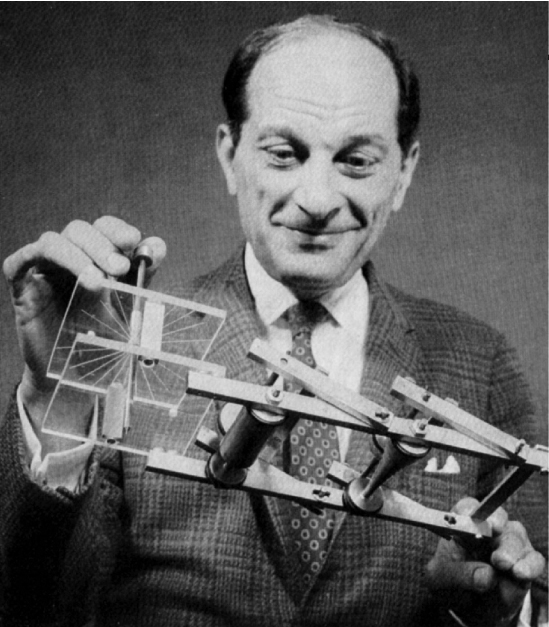
\includegraphics[width=0.9\columnwidth]{stanislaw.jpg}
    \end{column}
  \end{columns}
\end{frame}

\begin{frame}{História dos Métodos de Monte Carlo\footnote{para quem se interessou, a história se encontra em \textcite{eckhardtStanUlamJohn1987}}}
  \begin{columns}
    \begin{column}{0.8\textwidth}
      \begin{vfilleditems}
        \item A ideia do método veio enquanto jogava paciência durante sua
        recuperação de uma cirurgia, Ulam pensou em jogar centenas de jogos para
        estimar estatisticamente a probabilidade de um resultado bem-sucedido
        \item Ulam descreveu a ideia para John von Neumann em 1946
        \item \small Por ser secreto, o trabalho de von Neumann e Ulam exigia um codinome.
        Um colega de von Neumann e Ulam, Nicholas Metropolis, sugeriu usar o nome Monte Carlo,
        que se refere ao Casino Monte Carlo em Mônaco, onde o tio de Ulam (Michał Ulam)
        pedia dinheiro emprestado a parentes para jogar.
      \end{vfilleditems}
    \end{column}
    \begin{column}{0.2\textwidth}
      \centering
      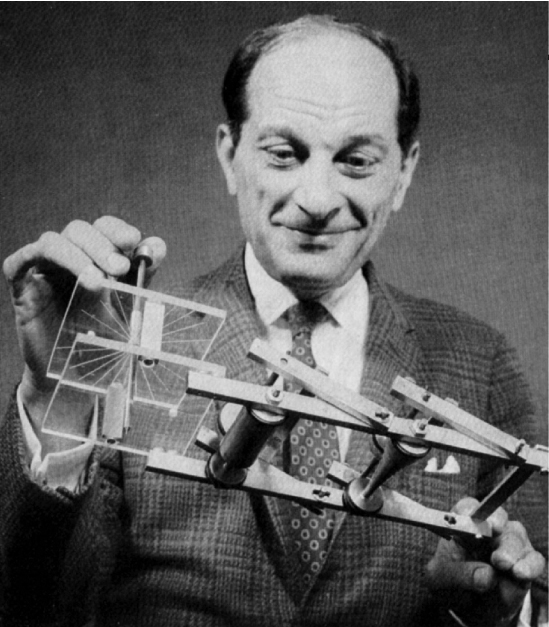
\includegraphics[width=0.9\columnwidth]{stanislaw.jpg}
    \end{column}
  \end{columns}
\end{frame}

\subsection{Por quê Precisamos de MCMC?}
\begin{frame}{Por quê Precisamos de MCMC?}
  A principal barreira computacional para estatística Bayesiana é o denominador
  $P(\text{data})$ da fórmula de Bayes:

  $$P(\theta \mid \text{data})=\frac{P(\theta) \cdot P(\text{data} \mid \theta)}{P(\text{data})}$$

  Em casos discretos podemos fazer o denominador virar a soma de todos os parâmetros
  usando a \textbf{regra da cadeia de probabilidade} (\textit{chain rule}):

  $$P(A,B \mid C)=P(A \mid B,C) \times P(B \mid C)$$

  Isto também é chamado de \textbf{marginalização}:

  $$P(\text{data})=\sum_{\theta} P(\text{data} \mid \theta) \times P(\theta)$$
\end{frame}

\begin{frame}{Por quê Precisamos de MCMC?}
  Porém no caso de valores contínuos o denominador $P(\text{data})$ vira uma integral
  bem grande e complicada de calcular:

  $$P(\text{data})=\int_{\theta} P(\text{data} \mid \theta) \times P(\theta)d \theta$$

  Em muitos casos essa integral vira \textit{intratável} (incalculável) e
  portanto devemos achar outras maneiras de calcular a probabilidade posterior
  $P(\theta \mid \text{data})$ de Bayes sem usar o denominador $P(\text{data})$.
  \vfill
  \Large \textbf{É aqui que entra Métodos de Monte Carlo!}
\end{frame}

\begin{frame}{Para quê serve o denominador $P(\text{data})$}
  Para normalizar a posterior com o intuito de torná-la uma distribuição
  probabilística válida. Isto quer dizer que a soma de todas as probabilidades
  dos eventos possíveis da distribuição devem ser iguais a $1$:
  \begin{vfilleditems}
    \item no caso de distribuição probabilística \textbf{discreta}:
    $$\sum_{\theta} P(\theta \mid \text{data}) = 1$$
    \item no caso de distribuição probabilística \textbf{contínua}:
    $$\int_{\theta} P(\theta \mid \text{data})d \theta = 1$$
  \end{vfilleditems}
\end{frame}

\begin{frame}{Se removermos o denominador de Bayes o que temos?}
  Ao removermos o denominador $(\text{data})$ temos que a posterior
  $P(\theta \mid \text{data})$ é \textbf{proporcional} à \textit{priori}
  multiplicada pela verossimilhança $P(\theta) \cdot P(\text{data} \mid \theta)$:

  $$P(\theta \mid \text{data}) \propto P(\theta) \cdot P(\text{data} \mid \theta)$$

\end{frame}

\subsubsection{Correntes Markov}
\begin{frame}{Método de Montecarlo com Correntes Markov -- (MCMC)}
  Aí que entra \textbf{Método Montecarlo com Correntes Markov}\footnote{do inglês
  \textit{Markov Chain Monte Carlo} (MCMC)}.
  \vfill
  MCMC é uma classe ampla de ferramentas computacionais para aproximação
  de integrais e geração de amostras de uma probabilidade posterior
  \parencite{brooksHandbookMarkovChain2011}.
  \vfill
  MCMC é usada quando não é possível coletar amostras de $\boldsymbol{\theta}$
  direto da distribuição probabilística posterior
  $P(\boldsymbol{\theta} \mid \text{data})$.
  Ao invés disso, nos coletamos amostras de maneira iterativa que a cada passo do
  processo nós esperamos que a distribuição da qual amostramos
  $P^*(\boldsymbol{\theta}^{(*)} \mid \text{data})$
  se torna cada vez mais similar à posterior $P(\boldsymbol{\theta} \mid \text{data})$.
  \vfill
  Tudo isso é para \textbf{eliminar o cálculo} (muitas vezes impossível) do \textbf{denominador} $P(\text{data})$.
\end{frame}

\begin{frame}{Correntes Markov}
  \begin{columns}
    \begin{column}{0.8\textwidth}
      \begin{vfilleditems}
        \item A ideia é \textbf{definir uma corrente Markov ergódica}
        (quer dizer que há uma distribuição estacionária única)
        dos quais o conjunto de estados possíveis é o espaço amostral e a
        distribuição estacionária é a distribuição a ser \textit{aproximada} (ou \textit{amostrada}).
        \item Seja $X_0, X_1, \dots, X_n$ uma simulação da corrente.
        A corrente Markov \textbf{converge à distribuição estacionária de qualquer
        estado inicial} $X_0$ após um \textbf{número suficiente grande de iterações} $r$,
        a distribuição do estado $X_r$ estará similar à distribuição estacionária,
        então podemos usá-la com amostra.
      \end{vfilleditems}
    \end{column}
    \begin{column}{0.2\textwidth}
      \centering
      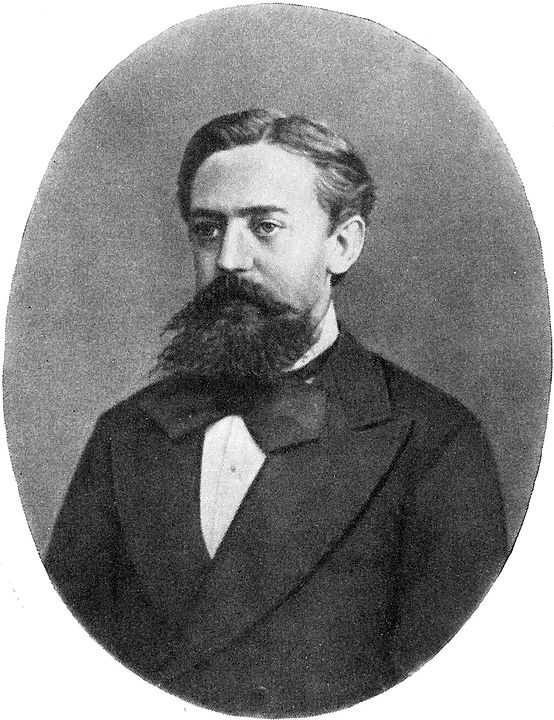
\includegraphics[width=0.9\columnwidth]{andrei_markov.jpg}
    \end{column}
  \end{columns}
\end{frame}

\begin{frame}{Correntes Markov}
  \begin{columns}
    \begin{column}{0.8\textwidth}
      \begin{vfilleditems}
        \item As correntes Markov possuem uma propriedade que a distribuição probabilística
        do próximo estado depende \textbf{apenas do estado atual e não na sequência
        de eventos que precederam}:
        $P(X_{n+1}=x \mid X_{0},X_{1},X_{2},\ldots ,X_{n}) = P(X_{n+1}=x \mid X_{n})$.
        Essa propriedade é chamada de \textbf{Markoviana}.
        \item Similarmente, repetindo esse argumento com $X_r$ como o ponto inicial,
        podemos usar $X_{2r}$ como amostra, e assim por diante.
        Podemos então usar a sequência de estados $X_r, X_{2r}, X_{3r}, \dots$
        como quase \textbf{amostras independentes} da distribuição estacionária da
        corrente Markov.
      \end{vfilleditems}
    \end{column}
    \begin{column}{0.2\textwidth}
      \centering
      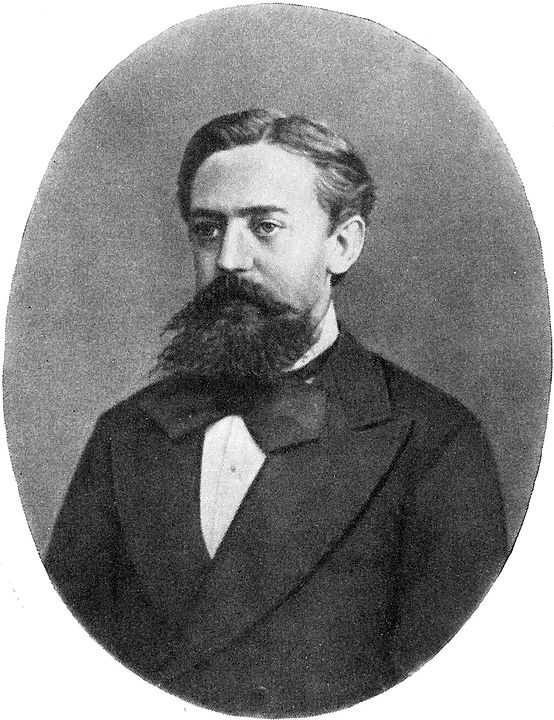
\includegraphics[width=0.9\columnwidth]{andrei_markov.jpg}
    \end{column}
  \end{columns}
\end{frame}

% Idea taken from http://steventhornton.ca/blog/markov-chains-in-latex.html
\begin{frame}{Exemplo de Corrente Markov}
  \centering
  \begin{tikzpicture}
    % Add the states
    \node[state,
    text=yellow,
    minimum size=2cm,
    thick
    ]
    (s) {Sol};
    \node[state,
    right=3cm of s,
    text=blue!30!white,
    minimum size=2cm,
    thick
    ]
    (r) {Chuva};

% Connect the states with arrows
\draw[every loop,
    auto=right,
    line width=1mm,
    >=latex]
  (s) edge[bend right, auto=left]  node {0.6} (r)
  (r) edge[bend right, auto=right] node {0.7} (s)
  (s) edge[loop above]             node {0.4} (s)
  (r) edge[loop above]             node {0.3} (r);
\end{tikzpicture}
\end{frame}

\begin{frame}{Correntes Markov}
  A eficácia dessa abordagem depende em:

  \begin{vfilleditems}
    \item \textbf{o quão grande $r$ deve ser} para garantir uma \textbf{amostra adequadamente boa}
    \item \textbf{poder computacional} requerido para cada iteração da corrente Markov.
  \end{vfilleditems}

  \vfill
  \footnotesize
  Além disso, é costumeiro descartarmos as primeiras iterações do algoritmo pois
  elas costumam não ser representativas da distribuição a ser aproximada.
  Nas iterações iniciais de algoritmos MCMC geralmente a corrente Markov
  está em um processo de aquecimento\footnote{Algumas referências chamam esse processo de \textit{burnin}}
  (\textit{warm-up}) e seu estado está bem distante do ideal para começarmos uma amostragem
  fidedigna.
  \vfill
  Geralmente, recomenda-se que se descarte metade das iterações \parencite{gelmanBasicsMarkovChain2013}.
\end{frame}

\subsection{Algoritmos de MCMC}
\begin{frame}{Algoritmos de MCMC}
  Temos \textbf{MUITOS} algoritmos de MCMC\footnote{Veja a \href{https://en.wikipedia.org/wiki/Markov_chain_Monte_Carlo}{página da Wikipedia para uma listagem completa}}
  Mas aqui vamos cobrir duas classes de algoritmos MCMC:
  \begin{vfilleditems}
    \item Metropolis-Hastings \parencite{metropolisEquationStateCalculations1953, hastingsMonteCarloSampling1970}

    \item Hamiltonian Monte Carlo\footnote{às vezes chamado de \textit{Hybrid Monte Carlo}, especialmente na literatura de Física} \parencite{neal2011mcmc, betancourtConceptualIntroductionHamiltonian2017}
  \end{vfilleditems}
\end{frame}

\begin{frame}{Classe de Algoritmos MCMC -- Metropolis-Hastings}
  Os primeiros algoritmos de MCMC. Usam uma regra de aceitação/rejeição das
  propostas. Caracterizados por propostas oriundas de um passeio aleatório\footnote{\textit{random walk}}
  no espaço amostral. O algoritmo de \textbf{Gibbs} pode ser visto como um
  \textbf{caso especial} do algoritmo de MH porque
  todas as propostas são aceitas \parencite{gelmanIterativeNonIterativeSimulation1992}
  \vfill
  Assintoticamente, possuem uma taxa de aceitação de 23.4\% e o custo de cada iteração é
  $\mathcal{O}(d)$, na qual $d$ é a dimensão do espaço amostral \parencite{beskosOptimalTuningHybrid2013}.
\end{frame}

\begin{frame}{Classe de Algortimos MCMC -- Hamiltonian Monte Carlo}
  Os algoritmos MCMC mais eficientes na atualidade. Tenta evitar o comportamento
  de passeio aleatório introduzindo um vetor de momento auxiliar e
  implementando dinâmicas Hamiltonianas. As propostas são "guiadas"~
  para regiões de maior densidade do espaço amostral. Isso faz com que HMC seja
  \textbf{ordens de magnitude mais eficiente que MH e Gibbs}.
  \vfill
  Assintoticamente, possuem uma taxa de aceitação de 65.1\% e o custo de cada iteração é
  $\mathcal{O}(d^{\frac{1}{4}})$, na qual $d$ é a dimensão do espaço amostral \parencite{beskosOptimalTuningHybrid2013}.
\end{frame}

\subsubsection{Metropolis}
\begin{frame}{Algoritmo de Metropolis}
  \begin{columns}
    \begin{column}{0.8\textwidth}
      O primeiro algoritmo MCMC amplamente utilizado para gerar amostras de
      correntes Markov foi originário na física na década de 1950 e chama-se Metropolis
      \parencite{metropolisEquationStateCalculations1953} em homenagem ao primeiro
      autor \href{https://en.wikipedia.org/wiki/Nicholas_Metropolis}{Nicholas Metropolis}.
      \vfill
      Em síntese, o algoritmo de Metropolis é uma adaptação de um passeio aleatório
      com uma regra de aceitação/rejeição para convergir à distribuição-alvo.
      \vfill
      O algorimo de Metropolis usa uma \textbf{distribuição de propostas}
      $J_t(\boldsymbol{\theta}^{(*)})$
      para definir próximos valores da distribuição
      $P^*(\boldsymbol{\theta}^{(*)} \mid \text{data})$.
      Essa distribuição deve ser simétrica:
      $$
      J_t (\boldsymbol{\theta}^{(*)} \mid \boldsymbol{\theta}^{(t-1)}) = J_t(\boldsymbol{\theta}^{(t-1)} \mid \boldsymbol{\theta}^{(*)})
      $$
    \end{column}
    \begin{column}{0.2\textwidth}
      \centering
      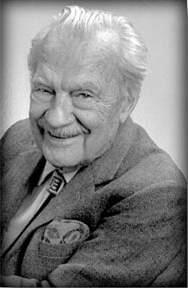
\includegraphics[width=0.9\columnwidth]{nicholas_metropolis.png}
    \end{column}
  \end{columns}
\end{frame}

\begin{frame}{Algoritmo de Metropolis}
  A essência do algoritmo é um passeio aleatório pelo espaço amostral dos parâmetros,
  onde a probabilidade da corrente Markov mudar de estado é definida como:

  $$
  P_{\text{mudar}} = \min\left({\frac{P (\boldsymbol{\theta}_{\text{proposto}})}{P (\boldsymbol{\theta}_{\text{atual}})}},1\right).
  $$

  Isso quer dizer a corrente Markov somente mudará para um novo estado em duas condições:
  \begin{vfilleditems}
    \small
    \item \small Quando a probabilidade dos parâmetros propostos pelo passeio aleatório
    $P(\boldsymbol{\theta}_{\text{proposto}})$ é \textbf{\textcolor{blue}{maior}}
    que a probabilidade dos parâmetros do estado atual
    $P(\boldsymbol{\theta}_{\text{atual}})$, mudamos com 100\% de probabilidade.

    \item \small Quando a probabilidade dos parâmetros propostos pelo passeio aleatório
    $P(\boldsymbol{\theta}_{\text{proposto}})$ é \textbf{\textcolor{red}{menor}}
    que a probabilidade dos parâmetros do estado atual
    $P(\boldsymbol{\theta}_{\text{atual}})$, mudamos com probabilidade igual a
    proporção dessa diferença.
  \end{vfilleditems}
\end{frame}

\begin{frame}[fragile]{Algoritmo de Metropolis}
    \SetAlCapFnt{\normalsize}
    \SetAlCapNameFnt{\normalsize}
    \begin{algorithm}[H]
    \DontPrintSemicolon
    \SetAlgoNoEnd
    \SetAlgoLined
    Defina um ponto inicial $\boldsymbol{\theta}^{(0)} \in \mathbb{R}^p$ do qual $P\left(\boldsymbol{\theta}^{(0)} \mid \boldsymbol{y} \right) > 0$\;
     \Para{$t = 1, 2, \dots$}{
      Amostra uma proposta $\boldsymbol{\theta}^{(*)}$ de uma distribuição de propostas no tempo $t$, $J_t \left(\boldsymbol{\theta}^{(*)} \mid \boldsymbol{\theta}^{(t-1)} \right)$\;
      Como regra de aceitação/rejeição calcule a proporção das probabilidades:
      $r = \frac{P\left(\boldsymbol{\theta}^{(*)}  \mid \boldsymbol{y} \right)}{P\left(\boldsymbol{\theta}^{(t-1)} \mid \boldsymbol{y} \right)}$\;
      Designe:
      $
        \boldsymbol{\theta}^{(t)} =
          \begin{cases}
          \boldsymbol{\theta}^{(*)} & \text{com probabilidade $\min(r,1)$}\\
          \boldsymbol{\theta}^{(t-1)} & \text{caso contrário}
        \end{cases}
      $\;
     }
     \caption{Metropolis}
    \end{algorithm}
\end{frame}

\begin{frame}{Intuição Visual de Metropolis}
\centering
    \begin{tikzpicture}
        \begin{axis}[every axis plot, line width=2pt,
            ylabel=PDF,
            domain=-4:4,samples=200,
            ymax = 0.6, ytick={0, 0.2, 0.4},
            axis x line*=bottom, % no box around the plot, only x and y axis
            axis y line*=left, % the * suppresses the arrow tips
            enlargelimits=true,
            ] % extend the axes a bit

            \addplot [blue] {gaussian(0, 1)};
            \node[inner sep=0pt] (hikerlower) at (-2,0.13){\Strichmaxerl[2pt]};
            \node[inner sep=0pt] (hikerupper) at (0,0.5){\Strichmaxerl[2pt]};
            \node[inner sep=0pt] (hikerlower2) at (2,0.13){\Strichmaxerl[2pt]};
            \draw[->, red, line width=2pt] (hikerlower) to [out=90,in=135] node[above left] {\large$P=1$} (hikerupper);
            \draw[->, yellow, line width=2pt] (hikerupper) to [out=45,in=135] node[right] {\large$P\approx\frac{0.1}{0.4}\approx\frac{1}{4}$} (hikerlower2);
        \end{axis}
        \end{tikzpicture}

\end{frame}

\subsubsection{Metropolis-Hastings}
\begin{frame}{Algoritmo de Metropolis}
  \begin{columns}
    \begin{column}{0.8\textwidth}
      Na década de 1970, surgiu um generalização do algoritmo de Metropolis
      que \textbf{não} necessita que as distribuições de proposta sejam simétricas:
      $$
      J_t (\boldsymbol{\theta}^{(*)} \mid \boldsymbol{\theta}^{(t-1)}) \neq J_t(\boldsymbol{\theta}^{(t-1)} \mid \boldsymbol{\theta}^{(*)})
      $$
      A generalização foi proposta por \href{https://en.wikipedia.org/wiki/W._K._Hastings}{Wilfred Keith Hastings}
      \parencite{hastingsMonteCarloSampling1970} e chama-se algoritmo
      de \textbf{Metropolis-Hastings}.
    \end{column}
    \begin{column}{0.2\textwidth}
      \centering
      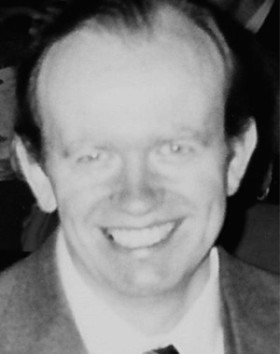
\includegraphics[width=0.9\columnwidth]{hastings.jpg}
    \end{column}
  \end{columns}
\end{frame}

\begin{frame}[fragile]{Algoritmo de Metropolis - Hastings}
    \SetAlCapFnt{\normalsize}
    \SetAlCapNameFnt{\normalsize}
    \small
    \begin{algorithm}[H]
    \DontPrintSemicolon
    \SetAlgoNoEnd
    \SetAlgoLined
    Defina um ponto inicial $\boldsymbol{\theta}^{(0)} \in \mathbb{R}^p$ do qual $P\left(\boldsymbol{\theta}^{(0)} \mid \boldsymbol{y} \right) > 0$\;
     \Para{$t = 1, 2, \dots$}{
      Amostra uma proposta $\boldsymbol{\theta}^{(*)}$ de uma distribuição de propostas no tempo $t$, $J_t \left(\boldsymbol{\theta}^{(*)} \mid \boldsymbol{\theta}^{(t-1)} \right)$\;
      Como regra de aceitação/rejeição calcule a proporção das probabilidades:
      $r = \frac{\frac{P \left(\boldsymbol{\theta}^{(*)} \mid \boldsymbol{y} \right)}{J_t \left(\boldsymbol{\theta}^{(*)} \mid \boldsymbol{\theta}^{(t-1)} \right)}}{\frac{P \left(\boldsymbol{\theta}^{(t-1)} \mid \boldsymbol{y} \right)}{J_t \left(\boldsymbol{\theta}^{(t-1)} \mid \boldsymbol{\theta}^{(*)} \right)}}$\;
      Designe:
      $
        \boldsymbol{\theta}^{(t)} =
          \begin{cases}
          \boldsymbol{\theta}^{(*)} & \text{com probabilidade $\min(r,1)$}\\
          \boldsymbol{\theta}^{(t-1)} & \text{caso contrário}
        \end{cases}
      $\;
     }
     \caption{Metropolis-Hastings}
    \end{algorithm}
\end{frame}

\begin{frame}{Animação Metropolis\footnote{veja Metropolis em ação no \href{https://chi-feng.github.io/mcmc-demo/app.html?algorithm=RandomWalkMH&target=banana}{\texttt{chi-feng/mcmc-demo}}}}
  \centering
  \movie[loop, width=9cm, height=6cm]{Animação Metropolis}{animations/rwmh.m4v}
\end{frame}

\subsubsection{Limitações dos Algoritmos Metropolis}
\begin{frame}{Limitações dos Algoritmos Metropolis}
  As limitações do algoritmo de Metropolis-Hastings são principalmente
  \textbf{computacionais}:
  \begin{vfilleditems}
    \item Com propostas geradas aleatoriamente, geralmente leva um grande número de
    iterações para entrar em áreas de densidade posterior mais alta (mais provável).

    \item Mesmo algoritmos de Metropolis-Hastings eficientes às vezes aceitam menos de
    25\% das propostas \parencite{robertsWeakConvergenceOptimal1997, beskosOptimalTuningHybrid2013}.

    \item Em situações dimensionais mais baixas, o poder computacional aumentado pode compensar a eficiência mais baixa até certo ponto.
    Mas em situações de modelagem de dimensões mais altas e mais complexas, computadores maiores
    e mais rápidos sozinhos raramente são suficientes para superar o desafio.
  \end{vfilleditems}
\end{frame}

\subsubsection{Gibbs}
\begin{frame}{Algoritmo de Gibbs}
  \begin{columns}
    \begin{column}{0.8\textwidth}
      Para contornar o problema de baixa taxa de aceitação dos algoritmos de Metropolis
      foi desenvolvido o algoritmo de Gibbs que
      \textbf{não possui uma regra de aceitação/rejeição}
      para a mudança de estado da corrente Markov:
      \textbf{Todas as propostas são aceitas}!
      \vfill
      O algoritmo de Gibbs teve ideia original concebida pelo físico Josiah Willard Gibbs
      em referência a uma analogia entre um algoritmo de amostragem e a
      física estatística (\textit{statistical physics} um ramo da física que tem sua
      base em mecânica estatística, \textit{statistical mechanics}).
      O algoritmo foi descrito pelos irmãos Stuart e Donald Geman em 1984
      \parencite{gemanStochasticRelaxationGibbs1984}, cerca de oito décadas após
      a morte de Gibbs.
    \end{column}
    \begin{column}{0.2\textwidth}
      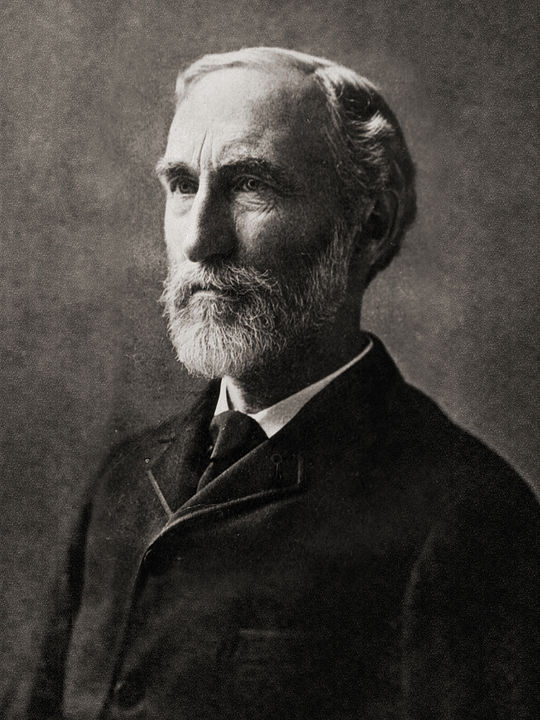
\includegraphics[width=0.9\columnwidth]{josiah_gibbs.jpg}
    \end{column}
  \end{columns}
\end{frame}

\begin{frame}{Algoritmo de Gibbs}
  O algoritmo de Gibbs é muito útil em espaços amostrais multidimensionais\footnote{
  no qual há bem mais que 2 parâmetros a serem amostrados da probabilidade posterior}.
  Também é conhecido como amostragem condicional alternativa
  (\textit{alternating conditional sampling}), pois amostramos sempre um parâmetro
  \textbf{condicionado} à probabilidade dos outros parâmetros do modelo.
  \vfill
  O algoritmo de Gibbs pode ser visto como um \textbf{caso especial} do algoritmo
  de Metropolis-Hastings porque todas as propostas são aceitas
  \parencite{gelmanIterativeNonIterativeSimulation1992}.
  \vfill
  A essência do algoritmo de Gibbs é a amostragem de parâmetros condicionada à outros parâmetros:
  $$P(\theta_1 \mid \theta_2, \dots \theta_p)$$
\end{frame}

\begin{frame}[fragile]{Algoritmo de Gibbs}
    \SetAlCapFnt{\normalsize}
    \SetAlCapNameFnt{\normalsize}
    \begin{algorithm}[H]
    \DontPrintSemicolon
    \SetAlgoNoEnd
    \SetAlgoLined
    Defina um ponto inicial $\boldsymbol{\theta}^{(0)} \in \mathbb{R}^p$ do qual $P\left(\boldsymbol{\theta}^{(0)} \mid \boldsymbol{y} \right) > 0$\;
     \Para{$t = 1, 2, \dots$}{
      Designe:
      $ \boldsymbol{\theta}^{(t)} =
        \begin{cases}
        \theta^{(t)}_1 &\sim P \left(\theta_1 \mid \theta^{(0)}_2, \dots, \theta^{(0)}_p \right) \\
        \theta^{(t)}_2 &\sim P \left(\theta_2 \mid \theta^{(t-1)}_1, \dots, \theta^{(0)}_p \right) \\
        &\vdots \\
        \theta^{(t)}_p &\sim P \left(\theta_p \mid \theta^{(t-1)}_1, \dots, \theta^{(t-1)}_{p-1} \right)
     \end{cases}
      $\;
     }
     \caption{Gibbs}
    \end{algorithm}
\end{frame}

\begin{frame}{Animação Gibbs\footnote{Veja Gibbs em ação no \href{https://chi-feng.github.io/mcmc-demo/app.html?algorithm=GibbsSampling&target=banana}{\texttt{chi-feng/mcmc-demo}}}}
  \centering
  \movie[loop, width=9cm, height=6cm]{Animação Gibbs}{animations/gibbs.m4v}
\end{frame}

\subsubsection{Limitações do Algoritmo de Gibbs}
\begin{frame}{Limitações do Algoritmo de Gibbs}
  A principal limitação do algoritmo de Gibbs é com relação a
  \textbf{amostragem condicional alternativa}:
  \begin{vfilleditems}
    \item Em Metropolis temos propostas aleatórias
    de uma distribuição de propostas na qual amostramos cada parâmetro
    \textbf{incondicionalmente} à outros parâmetros e de maneira \textbf{simultânea} usando a
    probabilidade conjunta desses parâmetros. As mudanças de estado da corrente
    Markov são então executadas \textbf{multidimensionalmente}.
    Isto provoca movimentos "\textbf{diagonais}"~multidimensionais.

    \item No caso do algoritmo de Gibbs essa movimentação se dá apenas em um
    único parâmetro, pois amostramos \textbf{sequencialmente} e
    \textbf{condicionalmente} à outros parâmetros.
    Isto provoca movimentos \textbf{horizontais/verticais} unidimensionais,
    mas nunca movimentos diagonais multidimensionais.
  \end{vfilleditems}
\end{frame}

\subsubsection{Hamiltonian Monte Carlo (HMC)}
\begin{frame}{Classe de Algoritmos MCMC - Hamiltoninan Monte Carlo (HMC)}
  \begin{columns}
    \begin{column}{0.8\textwidth}
      Os problemas de baixas taxas de aceitação de propostas das técnicas de
      Metropolis e do desempenho baixo do algoritmo de Gibbs em problemas
      multidimensionais nas quais a geometria da posterior é complexa
      fizeram com que surgisse uma nova técnica MCMC usando dinâmica Hamiltoniana
      (em homenagem ao físico irlandês
      \href{https://en.wikipedia.org/wiki/William_Rowan_Hamilton}{William Rowan Hamilton}.
    \end{column}
    \begin{column}{0.2\textwidth}
      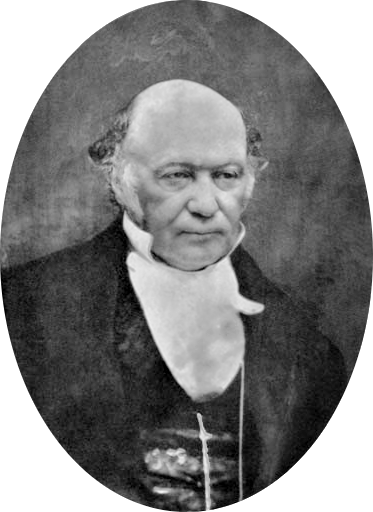
\includegraphics[width=0.9\columnwidth]{hamilton.png}
    \end{column}
  \end{columns}
\end{frame}

\begin{frame}{Algoritmo de HMC}
  O HMC é uma adaptação da técnica de Metropolis e emprega um esquema guiado de
  geração de novas proposta: isso melhora a taxa de aceitação de propostas e,
  consequentemente, a eficiência.
  \vfill
  Mais especificamente, o HMC usa o gradiente do log da posterior para direcionar
  a cadeia de Markov para regiões de maior densidade posterior,
  onde a maioria das amostras são coletadas.
  $$
  \frac{d \log P(\boldsymbol{\theta} \mid \boldsymbol{y})}{d \theta}
  $$
  Como resultado, uma corrente Markov com o algoritmo HMC bem ajustada aceitará
  propostas em uma taxa muito mais alta do que o algoritmo Metropolis tradicional
  \parencite{robertsWeakConvergenceOptimal1997, beskosOptimalTuningHybrid2013}.
\end{frame}

\begin{frame}{História do Algoritmo de HMC}
  HMC foi inicialmente descrito na literatura de física\footnote{que chamaram de \textit{"Hybrid"~Monte Carlo} -- HMC}
  \parencite{duaneHybridMonteCarlo1987}.
  \vfill
  Logo depois, HMC foi aplicado a problemas estatísticos por
  \textcite{nealImprovedAcceptanceProcedure1994} que chamou de \textit{Hamiltonean Monte Carlo}
  -- HMC).
  \vfill
  Para uma discussão aprofundada (que não é o foco deste conteúdo) de HMC eu recomendo
  \textcite{neal2011mcmc} e \textcite{betancourtConceptualIntroductionHamiltonian2017}.
\end{frame}

\begin{frame}{O que muda com HMC?}
  HMC usa dinâmica Hamiltoniana aplicada para partículas explorando de maneira mais
  eficiente a geometria de uma probabilidade posterior.
  \vfill
  Além de explorar melhor a geometria da posterior e tolerar geometrias complexas,
  HMC é muito mais eficiente que Metropolis e não sofre do problema de correlação
  dos parâmetros que Gibbs.
\end{frame}

\begin{frame}{Intuição por trás do Algoritmo de HMC}
  \small
  Para cada componente $\theta_j$, o HMC adiciona uma variável de momento
  $\phi_j$. A densidade posterior $P(\boldsymbol{\theta} \mid y)$ é incrementada
  por uma distribuição independente $P(\boldsymbol{\phi})$ dos momentos,
  definindo assim uma distribuição conjunta:
  $$
  P(\boldsymbol{\theta}, \boldsymbol{\phi} \mid y) = P(\boldsymbol{\phi}) \cdot P(\boldsymbol{\theta} \mid y)
  $$
  \small
  O HMC usa uma distribuição de propostas que muda dependendo do estado atual na
  corrente Markov. O HMC descobre a direção em que a distribuição posterior aumenta,
  chamada de \textit{gradiente}, e distorce a distribuição de propostas em
  direção ao \textit{gradiente}.
  \vfill
  A probabilidade da corrente Markov mudar de estado no algoritmo HMC é definida como:
  $$
  P_{\text{mudar}} = \min\left({\frac{P(\boldsymbol{\theta}_{\text{proposto}}) \cdot P(\boldsymbol{\phi}_{\text{proposto}})}{P(\boldsymbol{\theta}_{\text{atual}})\cdot P(\boldsymbol{\phi}_{\text{atual}})}}, 1\right)
  $$
\end{frame}

\begin{frame}{Distribuição dos Momentos -- $P(\boldsymbol{\phi})$}
  Normalmente damos a $\boldsymbol{\phi}$ uma distribuição normal multivariada
  com média 0 e covariância de $\mathbf{M}$,
  uma "matriz de massa".
  \vfill
  Para mantêr as coisas um pouco mais simples, usamos uma matriz de massa diagonal
  $\mathbf{M}$. Isso faz com que os componentes de $\boldsymbol{\phi}$ sejam
  independentes com
  $$\phi_j \sim \text{Normal}(0, M_{jj})$$
\end{frame}

\begin{frame}[fragile]{Algoritmo de HMC}
    \SetAlCapFnt{\normalsize}
    \SetAlCapNameFnt{\normalsize}
    \begin{algorithm}[H]
    \DontPrintSemicolon
    \SetAlgoNoEnd
    \SetAlgoLined
    \footnotesize
    Defina um ponto inicial $\boldsymbol{\theta}^{(0)} \in \mathbb{R}^p$ do qual $P\left(\boldsymbol{\theta}^{(0)} \mid \boldsymbol{y} \right) > 0$\;
    Amostre $\boldsymbol{\phi}$ de uma $\text{Normal}(\mathbf{0},\mathbf{M})$\;
    Simultaneamente amostre $\boldsymbol{\theta}^{(*)}$ e $\boldsymbol{\phi}$ com $L$ passos e tamanho de passo $\epsilon$.\;
    Defina o valor atual $\boldsymbol{\theta}$ como valor proposto $\boldsymbol{\theta}^{(*)}$:
    $\boldsymbol{\theta}^{(*)} \leftarrow \boldsymbol{\theta}$\;
    \Para{$1, 2, \dots, L$}{
     Use o gradiente do $\log$ da posterior de $\boldsymbol{\theta}^{(*)}$ para produzir um meio-passo de $\boldsymbol{\phi}$:
     $\boldsymbol{\phi} \leftarrow \boldsymbol{\phi} + \frac{1}{2} \epsilon \frac{d \log P(\boldsymbol{\theta}^{(*)} \mid \boldsymbol{y})}{d \theta}$\;
     Use $\boldsymbol{\phi}$ para atualizar $\boldsymbol{\theta}^{(*)}$:
     $\boldsymbol{\theta}^{(*)} \leftarrow \boldsymbol{\theta}^{(*)} + \epsilon \mathbf{M}^{-1} \boldsymbol{\phi}$\;
     Novamente use o gradiente de $\boldsymbol{\theta}$ para produzir um meio-passo de $\boldsymbol{\phi}$:
     $\boldsymbol{\phi} \leftarrow \boldsymbol{\phi} + \frac{1}{2} \epsilon \frac{d \log P(\boldsymbol{\theta}^{(*)} \mid \boldsymbol{y})}{d \theta}$\;
    }
    Como regra de aceitação/rejeição calcule:
    $r = \frac{P \left(\boldsymbol{\theta}^{(*)} \mid \boldsymbol{y} \right) P \left(\boldsymbol{\phi}^{(*)} \right)}{P \left(\boldsymbol{\theta}^{(t-1)} \mid \boldsymbol{y} \right) P \left(\boldsymbol{\phi}^{(t-1)} \right)}$\;
    Designe:
      $
        \boldsymbol{\theta}^{(t)} =
          \begin{cases}
          \boldsymbol{\theta}^{(*)} & \text{com probabilidade $\min(r,1)$}\\
          \boldsymbol{\theta}^{(t-1)} & \text{caso contrário}
        \end{cases}
      $\;
    \caption{Hamiltonian Monte Carlo (HMC)}
    \end{algorithm}
\end{frame}

\begin{frame}{Animação HMC\footnote{Veja HMC em ação no \href{https://chi-feng.github.io/mcmc-demo/app.html?algorithm=HamiltonianHMC&target=banana}{\texttt{chi-feng/mcmc-demo}}}}
  \centering
  \movie[loop, width=9cm, height=6cm]{Animação HMC}{animations/hmc.m4v}
\end{frame}

\begin{frame}{Um interlúdio de Integrador Numéricos}
  No campo das equações diferenciais ordinais temos a ideia de discretizar um
  sistema de equações diferenciais ordinais ao aplicar um pequeno passo $\epsilon$\footnote{algumas vezes também chamado de $h$}.
  Tais abordagem são chamadas de \textbf{integradores numéricos} e comportam uma
  \textbf{ampla classe} de ferramentas.
  \vfill
  O mais famoso e simples desses integradores numéricos é o método de Euler. No qual
  usa-se um tamamho de passo $\epsilon$ para calcular a solução numérica do estado
  em um futuro tempo $t$ a partir de condições iniciais específicas.
\end{frame}

\begin{frame}{Um interlúdio de Integrador Numéricos}
  \begin{columns}
    \begin{column}{0.6\textwidth}
      O problema é que o método de Euler quando aplicado para dinâmicas Hamiltonianas
      é que ele não preserva o volume. Uma das propriedades fundamentais das dinâmicas
      Hamiltonianas é que elas preservam volume, um resultado chamado de Teorema de
      Liouville. Isto faz com que o método de Euler seja uma péssima escolha como
      integrador numérico de um algoritmo HMC.
    \end{column}
    \begin{column}{0.4\textwidth}
      \begin{figure}
      \includegraphics[width=0.8\columnwidth]{euler_0_3.jpg}
      \caption{Método de Euler num algoritmo HMC com $\epsilon = 0.3$ e $L = 20$}
      \end{figure}
    \end{column}
  \end{columns}
\end{frame}

\begin{frame}{Um interlúdio de Integrador Numéricos\footnote{Um excelente livro-texto
  para integradores numéricos e integradores simpléticos é
  \textcite{irseles2008numericalanalysis}}}
  \begin{columns}
    \begin{column}{0.6\textwidth}
      Para preservação de volumes precisamos usar um
      \textbf{integrador simplético}. Integradores simpléticos são no máximo
      de ordem 2 e precisam ser usados com um tamanho de passo $\epsilon$ constante.
      Um dos principais integradores numéricos simpléticos usado em dinânimcas
      Hamiltonianas é o integrador \textbf{Störmer–Verlet}, também conhecido
      como \textit{leapfrog}.
    \end{column}
    \begin{column}{0.4\textwidth}
      \begin{figure}
        \includegraphics[width=0.8\columnwidth]{leapfrog_0_3.jpg}
        \caption{Integrador \textit{Leapfrog} num algoritmo HMC com $\epsilon = 0.3$ e $L = 20$}
        \end{figure}
    \end{column}
  \end{columns}
\end{frame}

\begin{frame}{Limitações do Algorito HMC}
  \begin{columns}
    \begin{column}{0.6\textwidth}
      Como vocês podem ver o algoritmo de HMC é muito sensível a escolhe da quantidade
      de passos $L$ e do tamanho do passo $\epsilon$. Em especial o integrador
      \textit{leapfrog} permite apenas um $\epsilon$ constante, portanto temos um
      equilíbrio delicado entre $L$ e $\epsilon$. Em  termos algorítmicos, $L$
      e $\epsilon$ são hiperparâmetros (tem que ser cuidadosamente ajustados).
    \end{column}
    \begin{column}{0.4\textwidth}
      \begin{figure}
        \includegraphics[width=0.8\columnwidth]{leapfrog_1_2.jpg}
        \caption{Integrador \textit{Leapfrog} num algoritmo HMC com $\epsilon = 1.2$ e $L = 20$}
        \end{figure}
    \end{column}
    \end{columns}
\end{frame}

\subsubsection{No-U-Turn-Sampler (NUTS)}
\begin{frame}{\textbf{N}o-\textbf{U}-\textbf{T}urn-\textbf{S}ampler (NUTS)}
  Em HMC, conseguimos ajustar o $\epsilon$ durante a execução do algoritmo. Mas, geralmente
  precisamos executar algumas vezes o amostrador HMC para ajustar o $L$.
  \vfill
  Aqui vem a ideia do \textbf{N}o-\textbf{U}-\textbf{T}urn-\textbf{S}ampler (NUTS)
  \parencite{hoffman2014no}.
  Não é preciso ajustar \textbf{nada} apenas "apertar"~o botão. Ele calcula automaticamente
  $\epsilon$ e $L$.
\end{frame}

\begin{frame}{\textbf{N}o-\textbf{U}-\textbf{T}urn-\textbf{S}ampler (NUTS)}
  Mais especificamente precisamos de um critério que informe que já simulamos as dinâmicas
  Hamiltonianas por "tempo suficiente". \textit{i.e.} simular as dinâmicas por mais tempo
  não aumentaria a distância entre a proposta $\boldsymbol{\theta}^{(*)}$ e o valor atual
  $\boldsymbol{\theta}$.
  \vfill
  NUTS então usa um critério baseado no produto interno entre os vetores do momento
  atual $\boldsymbol{\phi}$ e a diferença entre os vetores
  da proposta $\boldsymbol{\theta}^{(*)}$ e o valor atual $\boldsymbol{\theta}$,
  que é a derivada com respeito ao tempo $t$ de metade da distância ao quadrado
  entre $\boldsymbol{\theta}$ e $\boldsymbol{\theta}^{(*)}$
  $$
  (\boldsymbol{\theta}^{(*)} - \boldsymbol{\theta}) \cdot \boldsymbol{\phi}
  = (\boldsymbol{\theta}^{(*)} - \boldsymbol{\theta}) \cdot \frac{d}{dt} (\boldsymbol{\theta}^{(*)} - \boldsymbol{\theta})
  = \frac{d}{dt} \frac{(\boldsymbol{\theta}^{(*)} - \boldsymbol{\theta}) \cdot (\boldsymbol{\theta}^{(*)} - \boldsymbol{\theta})}{2}
  $$
\end{frame}

\begin{frame}{\textbf{N}o-\textbf{U}-\textbf{T}urn-\textbf{S}ampler (NUTS)}
  Isso sugere um algorimo que não permite com que as propostas sejam guiadas de maneira
  infinita até que a distância entre a proposta $\boldsymbol{\theta}^{(*)}$ e o valor atual
  $\boldsymbol{\theta}$ seja menor que zero.
  \vfill
  Isto quer dizer que tal algoritmo não \textbf{permitirá meia-voltas} (\textit{u-turns}).
\end{frame}

\begin{frame}{\textbf{N}o-\textbf{U}-\textbf{T}urn-\textbf{S}ampler (NUTS)}
  NUTS usa o integrador \textit{leapfrog} para criar uma árvore binária da qual os nós-folha
  são as posições do momento $\boldsymbol{\phi}$ traçando tanto um caminho para frente
  ($t+1$) quanto para trás ($t-1$) em um tempo fictício em um determinado tempo $t$.
  O crescimento dos nós-folha são \textbf{interrompidos} quando é detectado meia-volta
  tanto para frente quanto para trás.
  \begin{figure}
    \centering
    \includegraphics[width=0.6\textwidth]{nuts.jpg}
    \caption{NUTS crescendo nós-folha para frente}
  \end{figure}
\end{frame}

\begin{frame}{\textbf{N}o-\textbf{U}-\textbf{T}urn-\textbf{S}ampler (NUTS)}
  NUTS também um procedimento chamado \textit{Dual Averaging}
  \parencite{nesterov2009primal} para ajustar simultaneamente $\epsilon$ e $L$ ao
  considerar o produto $\epsilon \cdot L$.
  \vfill
  Tal ajuste é feito durante a fase de \textit{warmup} e os valores definidos de
  $\epsilon$ e $L$ são mantidos fixos durante a fase de amostragem.
\end{frame}

\begin{frame}{Algoritmo de NUTS}
    \SetAlCapFnt{\footnotesize}
    \SetAlCapNameFnt{\footnotesize}
    \begin{algorithm}[H]
    \DontPrintSemicolon
    \SetAlgoNoEnd
    \SetAlgoLined
    \fontsize{4.5pt}{6.5pt}\selectfont
    Defina um ponto inicial $\boldsymbol{\theta}^{(0)} \in \mathbb{R}^p$ do qual $P\left(\boldsymbol{\theta}^{(0)} \mid \boldsymbol{y} \right) > 0$\;
    \textcolor{blue}{Inicie uma árvore binária vazia com $2^L$ nós}\;
    Amostre $\boldsymbol{\phi}$ de uma $\text{Normal}(\mathbf{0},\mathbf{M})$\;
    Simultaneamente amostre $\boldsymbol{\theta}$ e $\boldsymbol{\phi}$ com $L$ passos e tamanho de passo $\epsilon$.\;
    Defina o valor atual $\boldsymbol{\theta}$ como valor proposto $\boldsymbol{\theta}^{(*)}$:
    $\boldsymbol{\theta}^{(*)} \leftarrow \boldsymbol{\theta}$\;
    \Para{$1, 2, \dots, 2L$}{
     \textcolor{blue}{Escolha uma direção $v \sim \text{Uniforme}\left( \left\{-1, 1 \right\} \right)$}\;
     Use o gradiente do $\log$ da posterior de $\boldsymbol{\theta}^{(*)}$ para produzir um meio-passo de $\boldsymbol{\phi}$ na direção $v$:
     $\boldsymbol{\phi} \leftarrow \boldsymbol{\phi} + v \frac{1}{2} \epsilon \frac{d \log P(\boldsymbol{\theta}^{(*)} \mid \boldsymbol{y})}{d \theta}$\;
     Use $\boldsymbol{\phi}$ para atualizar $\boldsymbol{\theta}^{(*)}$:
     $\boldsymbol{\theta}^{(*)} \leftarrow \boldsymbol{\theta}^{(*)} + \epsilon \mathbf{M}^{-1} \boldsymbol{\phi}$\;
     Novamente use o gradiente de $\boldsymbol{\theta}^{(*)}$ para produzir um meio-passo de $\boldsymbol{\phi}$ na direção $v$:
     $\boldsymbol{\phi} \leftarrow \boldsymbol{\phi} + v \frac{1}{2} \epsilon \frac{d \log P(\boldsymbol{\theta}^{(*)} \mid \boldsymbol{y})}{d \theta}$\;
     Defina o nó $L_t^v$ como a proposta $\boldsymbol{\theta}$\;
     \eSe{
       A diferença entre os vetores
       da proposta $\boldsymbol{\theta}^{(*)}$ e o valor atual $\boldsymbol{\theta}$ na direção $v$ for menor que zero: $v \frac{d}{dt} \frac{(\boldsymbol{\theta}^{(*)} - \boldsymbol{\theta}^{(*)}) \cdot (\boldsymbol{\theta}^{(*)} - \boldsymbol{\theta}^{(*)})}{2} < 0$\;
     }{
       \textcolor{red}{Pare a amostragem de $\boldsymbol{\theta}^{(*)}$ na direção $v$ e continue apenas amostrando na direção $-v$}\;
       }{
        \Se{A distância entre os vetores
        da proposta $\boldsymbol{\theta}^{(*)}$ e o valor atual $\boldsymbol{\theta}$ na direção restante $-v$ for menor que zero: $-v \frac{d}{dt} \frac{(\boldsymbol{\theta}^{(*)} - \boldsymbol{\theta}^{(*)}) \cdot (\boldsymbol{\theta}^{(*)} - \boldsymbol{\theta}^{(*)})}{2} < 0$\;
       }{
        \textcolor{red}{Pare a amostragem de $\boldsymbol{\theta}^{(*)}$\;
        }
       }
     }
    }
    Como regra de aceitação/rejeição calcule:
    $r = \frac{P \left(\boldsymbol{\theta}^{(*)} \mid \boldsymbol{y} \right) P \left(\boldsymbol{\phi}^{(*)} \right)}{P \left(\boldsymbol{\theta}^{(t-1)} \mid \boldsymbol{y} \right) P \left(\boldsymbol{\phi}^{(t-1)} \right)}$\;
    Designe:
      $
        \boldsymbol{\theta}^{(t)} =
          \begin{cases}
          \boldsymbol{\theta}^{(*)} & \text{com probabilidade $\min(r,1)$}\\
          \boldsymbol{\theta}^{(t-1)} & \text{caso contrário}
        \end{cases}
      $\;
    \caption{No-U-Turn-Sampler (NUTS)}
    \end{algorithm}
\end{frame}

\begin{frame}{Animação NUTS\footnote{Veja NUTS em ação no \href{https://chi-feng.github.io/mcmc-demo/app.html?algorithm=EfficientNUTS&target=banana}{\texttt{chi-feng/mcmc-demo}}}}
  \centering
  \movie[loop, width=9cm, height=6cm]{Animação NUTS}{animations/nuts.m4v}
\end{frame}

\subsubsection{Limitações de HMC e NUTS}
\begin{frame}{Limitações do Algorito HMC e NUTS - Funil de \textcite{nealSliceSampling2003}}
  O famoso funil da morte \footnote{muito comum em modelos hierárquicos}.
  Aqui vemos que os algoritmos HMC e NUTS, durante a exploração da
  posterior, tem que a todo momento trocar valores\footnote{lembre-se que
  $\epsilon$ e $L$ são definidos na fase de \textit{warmup} e
  mantidos fixos durante a fase de amostragem} de $\epsilon$ e $L$.
% https://crackedbassoon.com/writing/funneling
% import numpy as np
% import matplotlib
% import matplotlib.pyplot as plt
% from matplotlib import rcParams
% from scipy.stats import norm
% fs = rcParams["figure.figsize"]
% rcParams["figure.figsize"] = (fs[0], fs[0] / 2)
% rcParams["lines.linewidth"] = 2
% rcParams["font.size"] = 14
% rcParams["axes.edgecolor"] = 'b'
% rcParams["xtick.labelcolor"] = 'w'
% rcParams["ytick.labelcolor"] = 'w'


% # generate data
% np.random.seed(0)
% k = 9
% n = 10000
% v = norm.rvs(0, 3, n)
% x = norm.rvs(0, np.exp(v / 2), (k, n))

% # plot data and analytic log-likelihood
% r = 500
% x, v = np.meshgrid(np.linspace(-20, 20, r), np.linspace(-9, 9, r))
% logp = norm.logpdf(v, 0, 3) + norm.logpdf(x, 0, np.exp(v / 2))
% plt.imshow(logp, vmin=-7.5, vmax=-2.5, cmap="viridis", origin="lower")
% plt.xticks(np.linspace(0, 499, 5), labels=np.linspace(-20, 20, 5).astype(int))
% plt.yticks(np.linspace(0, 499, 5), labels=np.linspace(-9, 9, 5).astype(int))

% # save figure
% plt.savefig('slides/images/funnel.png', bbox_inches=0, transparent=True, dpi=300)
  \centering
  \includegraphics[width=0.65\textwidth]{funnel.png}
\end{frame}

\begin{frame}{Funil de \textcite{nealSliceSampling2003} e Parametrização Não-Centralizada\footnote{\textit{Non-Centered Parametrization} (NCP)}}
  \small
  O funil ocorre quando temos uma variável que a sua variância depende da variância
  de outra em uma escala exponencial. Um exemplo canônico de uma parametrização
  centralizada é:
  $$
  P(y,x) = \text{Normal}(y \mid 0 ,3) \cdot
  \text{Normal}\left(x \mid 0, e^{\left(\frac{y}{2}\right)}\right)
  $$
  Isto ocorre bastante em modelos hierárquicos, na relação dos \textit{prioris} de grupo
  com a(s) \textit{hiperpriori(s)} global(is). Então, reparametrizamos de maneira
  não-centrada alterando a geometria da posterior para facilitar a vida do amostrador
  MCMC:
  $$
  \begin{aligned}
    P(\tilde{y},\tilde{x}) &= \text{Normal}(\tilde{y} \mid 0, 1) \cdot
  \text{Normal}(\tilde{x} \mid 0, 1) \\
    y &= \tilde{y} \cdot 3 + 0 \\
    x &= \tilde{x} \cdot  e^{\left(\frac{y}{2}\right)} + 0
  \end{aligned}
  $$
\end{frame}

\begin{frame}{\href{https://mc-stan.org}{\texttt{Stan}} e NUTS}
  \href{https://mc-stan.org}{\texttt{Stan}} foi o primeiro amostrador MCMC a
  implementar NUTS. Além disso tem uma rotina otimizada automática de ajuste de $L$
  e $\epsilon$ durante a fase de \textit{warmup}. Possui os seguintes valores como
  hiperparâmetros padrões do NUTS\footnote{para mais informações sobre como
  modificar esses hiperparâmetros consulte a \href{
    https://mc-stan.org/docs/reference-manual/hmc-algorithm-parameters.html}{
    Seção 15.2 do \textit{Stan Reference Manual}}}:
  \begin{vfilleditems}
    \item \textbf{Taxa-alvo de aceitação de propostas Metropolis}: \lstinline!adapt_delta = 0.8!
    \item \textbf{Profundidade máxima de árvore} (em potências de 2): \lstinline!max_treedepth = 10! (quer dizer $2^{10} = 1024$)
  \end{vfilleditems}
\end{frame}

\subsection{Convergência de Correntes Markov}
\begin{frame}{Convergência de Correntes Markov}
  MCMC tem uma propriedade interessante que é garantido que \textbf{assintoticamente ele convergirá
  à distribuição-alvo}.
  \vfill
  Ou seja, se tivermos todo o tempo do mundo, é garantido que, irrelevante da geometria
  da distribuição-alvo (posterior), \textbf{MCMC irá lhe dar a resposta correta}.
  \vfill
  Porém não temos todo o tempo do mundo. Diferentes algoritmos MCMC, como HMC e NUTS,
  podem reduzir o tempo de amostragem (e \textit{warmup}) necessários para convergência.
\end{frame}

\subsubsection{Métricas de Convergência}
\begin{frame}{Métricas de Convergência}
  Temos algumas maneiras de mensurar se as correntes Markov convergiram à distribuição-alvo,
  \textit{i.e.} são "confiáveis":
  \begin{vfilleditems}
    \item Número de Amostras Efetivas (\textit{Effective Sample Size} -- ESS):
    uma aproximação do "número de amostras independentes"~geradas por uma corrente Markov.
    \item $\widehat{R}$ (\textit{Rhat}):
    escala de \textbf{R}edução potencial, uma métrica de mensuração que as correntes
    Markov se "misturaram", e, potencialmente, convergiram
  \end{vfilleditems}
\end{frame}

\begin{frame}{Métricas de Convergência - \textit{Effective Sample Size} \parencite{gelman2013bayesian}}
  $$\widehat{n}_{\text{eff}} = \frac{mn}{1 + \sum_{t=1}^T \widehat{\rho}_t}$$
  Onde:
  \begin{vfilleditems}
    \item $m$: número de correntes Markov
    \item $n$: amostras totais por corrente Markov (descontando \textit{warmup})
    \item $\widehat{\rho}_t$: uma estimativa de autocorrelação
  \end{vfilleditems}
\end{frame}

\begin{frame}{Métricas de Convergência - \textit{Rhat} \parencite{gelman2013bayesian}}
  $$\widehat{R} = \sqrt{\frac{\widehat{\text{var}}^+(\psi \mid y)}{W}}$$
  onde a $\widehat{\text{var}}^+(\psi \mid y)$ é a variância das amostras das
  correntes Markov para um determinado parâmetro $\psi$ sob uma média ponderada
  das variâncias intra-correntes (\textit{within-chain}) $W$ e inter-correntes
  (\textit{between-chain}) $B$
  $$\widehat{\text{var}}^+(\psi \mid y) = \frac{n-1}{n} W + \frac{1}{n} B$$
  Intuitivamente, seu valor é $1.0$ se as correntes estiverem totalmente convergentes.
  Como uma heurística, se $\widehat{R}$ for maior que $1.1$, você deve se preocupar pois
  provavelmente as correntes não tenham convergido adequadamente.
\end{frame}

\subsubsection{Visualizações de Convergência}
\begin{frame}{\textit{Traceplot} -- Correntes Markov Convergentes}
  \begin{figure}
    \centering
    \resizebox{.4\linewidth}{!}{\input{images/good_chains_traceplot.tex}}
  \end{figure}
\end{frame}

\subsubsection{O que fazer se Correntes Markov não Convergirem}

\begin{frame}[fragile]{\textit{Rhat} -- Mensagens de Erro do \href{https://mc-stan.org}{\texttt{Stan}}\footnote{além disso não deixe de checar o \href{https://mc-stan.org/misc/warnings.html}{guia dos \textcolor{red}{\textit{warnings}} do \texttt{Stan}}}}
  \begin{lstlisting}[basicstyle=\footnotesize\color{red}]
Warning messages:
1: There were 275 divergent transitions after warmup. See
http://mc-stan.org/misc/warnings.html#divergent-transitions-after-warmup
to find out why this is a problem and how to eliminate them.
2: Examine the pairs() plot to diagnose sampling problems

3: The largest R-hat is 1.12, indicating chains have not mixed.
Running the chains for more iterations may help. See
http://mc-stan.org/misc/warnings.html#r-hat
4: Bulk Effective Samples Size (ESS) is too low, indicating posterior
means and medians may be unreliable.
Running the chains for more iterations may help. See
http://mc-stan.org/misc/warnings.html#bulk-ess
5: Tail Effective Samples Size (ESS) is too low, indicating posterior
variances and tail quantiles may be unreliable.
Running the chains for more iterations may help. See
http://mc-stan.org/misc/warnings.html#tail-ess
  \end{lstlisting}
\end{frame}
% https://mc-stan.org/misc/warnings.html

\begin{frame}{\textit{Traceplot} -- Correntes Markov Divergentes}
  \begin{figure}
    \centering
    \resizebox{.4\linewidth}{!}{\input{images/bad_chains_traceplot.tex}}
  \end{figure}
\end{frame}

\begin{frame}{O que fazer se Correntes Markov não Convergirem}
  \textbf{Primeiro}: Antes de fazer ajustes finos no número de correntes
  \texttt{chains} ou no número de iterações \texttt{iter} (entre outros ...)
  saiba que o amostrador HMC-NUTS do \href{https://mc-stan.org}{\texttt{Stan}} e
  seu ecossistema de pacotes (\href{http://mc-stan.org/rstanarm/}{\texttt{rstanarm}} e
  \href{https://paul-buerkner.github.io/brms/}{\texttt{brms}} inclusos) é \textbf{muito
  eficiente e eficaz em explorar as mais diversas complexas e "malucas"~geometrias}
  de distribuições-alvo posterior.
  \vfill
  Os argumentos padrões, \texttt{iter = 2000}, \texttt{chains = 4} e
  \texttt{warmup = floor(iter / 2)}, funcionam perfeitamente para 99\% dos casos
  (mesmo em modelos complexos).
\end{frame}

\begin{frame}{O que fazer se Correntes Markov não Convergirem}
  \vfill
  Dito isto, \textbf{na maioria das vezes quando você
  possui problemas de amostragem e computacionais no seu modelo Bayesiano, o problema
  está na especificação do modelo e não no algoritmo de amostragem MCMC}\footnote{Esta
  frase foi dita por Andrew Gelman (o "pai"~do \texttt{Stan}) e é conhecido como o
  \textit{Folk Theorem} \parencite{gelmanFolkTheoremStatistical2008}:
  \textit{"When you have computational problems, often there’s a problem with
  your model"}}
\end{frame}

\begin{frame}{O que fazer se Correntes Markov não Convergirem}
  Se o seu modelo Bayesiano está com problemas de convergência há alguns
  passos que podem ser tentados\footnote{além disso,
  vale a pena ativar a decomposição QR na matriz $\mathbf{X}$ de dados, criando uma
  base ortogonal (não correlacionada) para amostragem. Isso faz com a distribuição-alvo
  (posterior) fique muito mais amigável do ponto de vista topológico/geométrico
  para o amostrador MCMC explorá-la de maneira mais eficiente e eficaz.}.
  Aqui listados do mais simples para o mais complexo:
  \begin{vfilleditems}
    \item \textbf{Aumentar o número de iterações e correntes}: primeira opção
    é aumentar o número de iterações do MCMC com o argumento \texttt{iter = XXX}
    e também é possível aumentar o número de correntes com o argumento
    \texttt{chains = X}. Lembrando que o padrão é \texttt{iter = 2000} e
    \texttt{chains = 4}.
  \end{vfilleditems}
\end{frame}

\begin{frame}{O que fazer se Correntes Markov não Convergirem}
  \begin{vfilleditems}
    \item \textbf{Alterar a rotina de adaptação do HMC}: a segunda opção é fazer com
    que o algoritmo de amostragem HMC fique mais conservador
    (com proposições de pulos menores). Isto pode ser alterado com o argumento
    \texttt{adapt\_delta} da lista de opções \texttt{control}.
    \texttt{control = list(adapt\_delta = 0.9)}. O padrão do \texttt{adapt\_delta} é $0.8$.
    Então qualquer valor entre $0.8$ e $1.0$ o torna mais conservador.
    \item \textbf{Reparametrização do Modelo}: a terceira opção é reparametrizar o
    modelo. Há duas maneiras de parametrizar o modelo: a primeira com parametrização
    centrada (\textit{centered parameterization}) e a segunda com parametrização
    não-centrada (\textit{non-centered parameterization}).
  \end{vfilleditems}
\end{frame}

\begin{frame}{O que fazer se Correntes Markov não Convergirem}
  \begin{vfilleditems}
    \item \textbf{Coletar mais dados}: às vezes o modelo é complexo demais e
    precisamos de uma amostragem maior para conseguirmos estimativas estáveis.
    \item \textbf{Repensar o modelo}: falha de convergência quando temos uma
    amostragem adequada geralmente é por conta de uma especificação de \textit{prioris} e
    verossimilhança que não são compatíveis com os dados. Nesse caso, é preciso
    repensar o processo generativo de dados no qual os pressupostos do modelo
    estão ancorados.
  \end{vfilleditems}
\end{frame}

\section{Comparação de Modelos}

\subsection{Leituras Recomendadas}
\begin{frame}{Comparação de Modelos - Leituras Recomendadas}
	\begin{vfilleditems}
		\item \textcite{gelman2013bayesian} - Capítulo 7: Evaluating, comparing, and expanding models
		\item \textcite{gelman2020regression} - Capítulo 11, Seção 11.8: Cross validation
		\item \textcite{mcelreath2020statistical} - Capítulo 7, Seção 7.5: Model comparison
		\item \textcite{vehtariPracticalBayesianModel2015}
		\item Tutorial do \texttt{loo} de \textcite{loo}
		\item \textcite{storopoli2021estatisticabayesianaR} - Comparação de Modelos
		\item \textcite{spiegelhalter2002bayesian}
		\item \textcite{van2005dic}
		\item \textcite{watanabe2010asymptotic}
		\item \textcite{gelfand1996model}
		\item \textcite{watanabe2010asymptotic}
		\item \textcite{geisser1979predictive}
	\end{vfilleditems}
\end{frame}

\subsection{Por quê Comparar Modelos?}
\begin{frame}{Por quê Comparar Modelos?}
	Depois de estimarmos um modelo Bayesiano,
	muitas vezes queremos medir sua precisão preditiva, por si só ou para
	fins de comparação, seleção ou cálculo de média do modelo \parencite{geisser1979predictive}.
\end{frame}

\begin{frame}{Mas, e as Verificações Preditivas da Posterior?}
	É uma maneira subjetiva e arbitrária de analisarmos e compararmos modelos
	entre si usando sua precisão preditiva.
	\vfill
	Há uma maneira objetiva de compararmos modelos Bayesianos com uma
	métrica robusta que nos ajude a selecionar qual o melhor modelo dentre o rol
	de modelos candidatos.
	\vfill
	Ter uma maneira objetiva de comparar modelos e escolher o melhor dentre eles
	é muito importante pois no \textit{workflow} Bayesiano geralmente temos diversas
	iterações entre \textit{prioris} e funções de verossimilhança o que ocasiona na
	criação de diversos modelos diferentes \parencite{gelmanBayesianWorkflow2020}.
\end{frame}

\subsection{Técnicas de Comparação de Modelos}
\begin{frame}{Técnicas de Comparação de Modelos}
	Temos diversas técnicas de comparação de modelos que usam a precisão preditiva,
	sendo as principais:
	\begin{vfilleditems}
		\item \textit{Leave-one-out cross-validation} (LOO)
		\parencite{vehtariPracticalBayesianModel2015}
		\item \textit{Deviance Information Criterion} (DIC)
		\parencite{spiegelhalter2002bayesian},  mas sabe-se que tem alguns problemas,
		que surgem em parte por não ser totalmente Bayesiano,
		pois se baseia em uma estimativa pontual \parencite{van2005dic}
		\item \textit{Widely Applicable Information Criteria} (WAIC)
		\parencite{watanabe2010asymptotic}, totalmente Bayesiano no sentido
		de que usa toda a distribuição posterior, e é assintoticamente igual ao
		LOO \parencite{vehtariPracticalBayesianModel2015}
	\end{vfilleditems}
\end{frame}

\begin{frame}{Interlúdio Histórico}
	\small
	Antigamente, não havia esse poder computacional e abundância de dados.
	Comparação de modelos eram baseados em uma métrica de divergência teórica
	oriunda da entropia da teoria da informação:
	$$
		H(p) = - \operatorname{E}\log(p_i) = -\sum^N_{i=1} p_i \log(p_i)
	$$
	\small
	Calculamos a divergência\footnote{\textit{divergence}} multiplicando por
	$-2$\footnote{razões históricas},
	então menores valores são melhores:
	$$
		D(y, \boldsymbol{\theta}) = -2 \cdot \underbrace{\sum^N_{i=1} \log \frac{1}{S}\sum^S_{s=1} P(y_i \mid \boldsymbol{\theta}^s)}_{\text{\textit{log pointwise predictive density} -- lppd}}
	$$
	\footnotesize
	onde $N$ é o tamanho da amostra e $S$ é o número de amostras simuladas da posterior.
\end{frame}

\begin{frame}{Interlúdio Histórico -- AIC \parencite{akaike1998information}}
	$$\text{AIC} = D(y, \boldsymbol{\theta}) + 2k = -2 \text{lppd}_{\text{mle}} + 2k$$
	onde $k$ é o número de parâmetros livres do modelo e $\text{lppd}_{\text{mle}}$ é
	a estimação de máxima verossimilhança (MLE) da lppd.
	\vfill
	AIC é uma aproximação que somente pode ser confiável quando:
	\begin{vfilleditems}
		\item As \textit{prioris} são uniformes (\textit{flat priors}) ou dominadas totalmente pela função de verossimilhança
		\item A posterior é aproximadamente uma distribuição Gaussiana/normal multivariada
		\item O tamanho da amostra $N$ é muito maior que número de parâmetros livres $k$: $N \gg k$
	\end{vfilleditems}
\end{frame}

\begin{frame}{Interlúdio Histórico -- DIC \parencite{spiegelhalter2002bayesian}}
	Uma generalização do AIC, onde substituímos a estimação de máxima verossimilhança
	pela média da posterior e $k$ por uma correção de viés baseada nos dados:
	$$
		DIC = D(y, \boldsymbol{\theta}) + k_{\text{DIC}} = -2 \text{lppd}_{\text{Bayes}}
		+2 \underbrace{\left( \text{lppd}_{\text{Bayes}} - \frac{1}{S} \sum^S_{s=1} \log P(y \mid \boldsymbol{\theta}^s) \right)}_{\text{$k$ corrigido de viés}}
	$$
	DIC remove a restrição das \textit{prioris} uniformes de AIC, mas mesmo assim
	mantém os presupostos da posterior ser uma distribuição Gaussiana/normal multivariada
	e que $N \gg k$
\end{frame}

\subsubsection{Precisão Preditiva}
\begin{frame}{Precisão Preditiva}
	Com o poder computacional que temos hoje não precisamos de aproximações\footnote{AIC, DIC etc.}.
	\vfill
	Podemos discutir métricas objetivas de \textbf{precisão preditiva}.
	\vfill
	Mas antes vamos definir o que é precisão preditiva.
\end{frame}

\begin{frame}{Precisão Preditiva}
	\begin{defn}[Precisão Preditiva]
		Bayesianos mensuram precisão preditiva usando simulações da distribuição posterior
		$\tilde{y}$ do modelo. Para isso temos a distribuição preditiva posterior
		(\textit{predictive posterior distribution}):
		$$
			p(\tilde{y} \mid y) = \int p(\tilde{y}_i \mid \theta) p(\theta \mid y) d \theta
		$$
		\small
		Onde $p(\theta \mid y)$ é a distribuição posterior do modelo\footnote{aquela
			que o \texttt{rstanarm} e \texttt{brms} estima para nós}.
		A fórmula acima significa que calculamos a integral de toda a
		probabilidade conjunta da distribuição posterior preditiva com a
		distribuição posterior do nosso modelo
		\normalsize
		Quanto \textbf{maior} a distribuição preditiva posterior
		$p(\tilde{y} \mid y)$ \textbf{melhor} será a precisão preditiva do modelo.
	\end{defn}
\end{frame}

\begin{frame}{Precisão Preditiva}
	Para mantermos comparabilidade entre amostras, calculamos a
	esperança dessa medida\footnote{do inglês \textit{expectation} que pode ser
		também interpretada como a média ponderada} para cada uma das $N$ observações
	da amostra:

	$$
		\operatorname{elpd} = \sum_{i=1}^N \int p_t(\tilde{y}_i) \log p(\tilde{y}_i \mid y) d \tilde{y}
	$$

	onde $\operatorname{elpd}$ é esperança do log da densidade preditiva pontual
	(\textit{expected log pointwise predictive density}) e
	$p_t(\tilde{y}_i)$ é a distribuição representando o verdadeiro processo
	generativo dos dados para $\tilde{y}_i$.
	Os $p_t(\tilde{y}_i)$ são desconhecidos e geralmente usamos validação
	cruzada\footnote{\textit{Cross Validation}} ou aproximação para
	a estimação da $\operatorname{elpd}$.
\end{frame}

\subsubsection{\textit{Leave-One-Out Cross-Validation} (LOO)}
\begin{frame}{\textit{Leave-One-Out Cross-Validation} (LOO)}
	Podemos calcular a $\operatorname{elpd}$ usando LOO
	\parencite{vehtariPracticalBayesianModel2015}:
	$$
		\operatorname{elpd}_{\text{loo}} = \sum_{i=1}^N \log p(y_i \mid y_{-i})
	$$
	onde
	$$
		p(y_i \mid y_{-i}) = \int p(y_i \mid \theta) p(\theta \mid y_{-i}) d \theta
	$$
	que é a densidade preditiva com uma observação a menos condicionada nos
	dados sem a observação $i$ ($y_{-i}$). Quase sempre usamos a aproximação
	PSIS-LOO\footnote{mais sobre isso já já...} pela sua robustez e baixo custo
	computacional.
\end{frame}

\subsubsection{\textit{Widely Applicable Information Criteria} (WAIC)}
\begin{frame}{\textit{Widely Applicable Information Criteria} (WAIC)}
	\footnotesize
	WAIC \parencite{watanabe2010asymptotic}, assim como o LOO também é uma
	abordagem alternativa para calcularmos a $\operatorname{elpd}$ e é definida como:

	$$
		\widehat{\operatorname{elpd}}_{\text{waic}} = \widehat{\operatorname{lppd}} - \widehat{p}_{\text{waic}}
	$$

	onde $\widehat{p}_{\text{waic}}$ é o número estimado efetivo de paramêtros e
	calculado com base em:

	$$
		\widehat{p}_{\text{waic}} = \sum_{i=1}^N \operatorname{var}_{\text{post}} (\log p(y_i \mid \theta))
	$$

	que conseguimos calcular usando a variância posterior do log da densidade preditiva para cada observação $y_i$:

	$$
		\widehat{p}_{\text{waic}} = \sum_{i=1}^N V^S_{s=1} (\log p(y_i \mid \theta^s))
	$$
	onde $V^S_{s=1}$ representa a variância da amostra:

	$$
		V^S_{s=1} a_s = \frac{1}{S-1} \sum^S_{s=1} (a_s - \bar{a})^2
	$$
\end{frame}

\subsubsection{\textit{K-fold Cross-Validation} (K-fold CV)}
\begin{frame}{\textit{K-fold Cross-Validation} (K-fold CV)}
	Da mesma maneira que conseguimos cacular a $\operatorname{elpd}$ usando LOO
	com $N-1$ partições da amostra podemos também calcular com qualquer número de
	partições que quisermos.
	\vfill
	Tal abordagem é chamada de \textbf{validação cruzada usando $K$ partições}
	(\textit{$K$-fold Cross-Validation}, encurtado para \textit{$K$-fold CV}).
	\vfill
	Ao contrário de LOO, não conseguimos aproximar a
	$\operatorname{elpd}$ usando \textit{$K$-fold CV} e precisamos fazer a computação
	atual da $\operatorname{elpd}$ sobre $K$ partições que quase sempre envolve
	um \textbf{alto custo computacional}.
\end{frame}

\subsection{\textit{Pareto Smoothed Importance Sampling} LOO (PSIS-LOO)}
\begin{frame}{\textit{Pareto Smoothed Importance Sampling} LOO (PSIS-LOO)}
	O PSIS usa \textbf{amostragem de importância}\footnote{\textit{importance sampling}},
	o que significa apenas que usa a abordagem de pesos de importância.
	\vfill
	A \textbf{suavização de Pareto} é uma técnica para tornar os pesos de importância
	mais confiáveis.
\end{frame}
\begin{frame}{Amostragem de Importância (\textit{Importance Sampling})}
	Se as $N$ amostras são condicionalmente independentes\footnote{ou seja
		são independentes condicionadas aos parâmetros do modelo, que é o pressuposto
		básico de qualquer modelo probabilístico Bayesiano} \parencite{gelfand1992model}
	podemos avaliar LOO com amostras $\boldsymbol{\theta}^s$ da posterior
	$P(\theta \mid y)$ usando \textbf{pesos de importância}:
	$$
		r_i^s=\frac{1}{P(y_i|\theta^s)} \propto \frac{P(\theta^s|y_{-i})}{P(\theta^s|y)}
	$$
	Para então conseguirmos \textit{Importance Sampling Leave-One-Out} (IS-LOO):
	$$
		P(\tilde{y}_i|y_{-i})
		\approx
		\frac{\sum_{s=1}^S r_i^s P(\tilde{y}_i|\theta^s)}{\sum_{s=1}^S r_i^s}
	$$
\end{frame}

\begin{frame}{Amostragem de Importância (\textit{Importance Sampling})}
	Porém a posterior $P(\theta \mid y)$ geralmente possui baixa variância e caudas
	mais curtas que as distribuições LOO $P(\theta \mid y_{-1})$ então se usarmos:
	$$
		P(\tilde{y}_i|y_{-i}) \approx \frac{\sum_{s=1}^S r_i^s P(\tilde{y}_i|\theta^s)}{\sum_{s=1}^S r_i^s}
	$$
	podemos gerar instabilidades pois os $r_i$ podem ter variância alta ou até infinita.
\end{frame}

\begin{frame}{Amostragem de Importância com Suavização de Pareto \textit{Pareto Smoothed Importance Sampling}}
	Podemos aprimorar a estimativa IS-LOO usando uma \textbf{suavização de Pareto}
	(\textit{Pareto Smoothed Importance Sampling}) \parencite{vehtariPracticalBayesianModel2015}
	\vfill
	Quando a cauda da distribuição dos pesos de importância é longa, um uso direto
	da amostragem de importância é sensível a um ou alguns valores grandes.
	Ajustando uma distribuição de Pareto generalizada à cauda superior dos pesos de
	importância, suavizamos esses valores.
\end{frame}
\begin{frame}{\textit{Pareto Smoothed Importance Sampling} LOO (PSIS-LOO)}
	Por fim temos PSIS-LOO:
	$$
		\widehat{\operatorname{elpd}}_{\rm psis-loo} =
		\sum_{i=1}^n \log
		\left(\frac{\sum_{s=1}^S w_i^s P(y_i|\theta^s)}{\sum_{s=1}^Sw_i^s} \right)
	$$
	onde $w$ é o peso truncado.
\end{frame}

\begin{frame}{\textit{Pareto Smoothed Importance Sampling} LOO (PSIS-LOO)}
	\small
	Usamos o parâmetro estimado de forma $\widehat{k}$ da distribuição de Pareto
	dos pesos de importância para avaliar a confiabilidade da estimativa:
	\begin{vfilleditems}
		\item \small $k < \frac{1}{2}$ a variância dos pesos de importância é finita,
		o teorema do limite central se mantém, e a estimativa converge rapidamente
		\item \small $\frac{1}{2} < k < 1$ a variância dos pesos de importância é infinitas,
		mas a média existe, o teorema do limite central generalizado
		para distribuições estáveis se mantém, e a convergência da estimativa é mais
		lenta
		A variação da estimativa PSIS é finita, mas pode ser grande.
		\item \small $k > 1$ a variância e a média da distribuição de pesos de importância não
		existe. A variação da estimativa PSIS é finita, mas pode ser grande
	\end{vfilleditems}
	\vfill
	\small
	Qualquer valor de $\widehat{k}$ maior que $0.5$ é sinal de alerta mas na prática
	ainda há um bom desempenho com $\widehat{k}$ até $0.7$
\end{frame}

\subsection{Comparação de Modelos no \texttt{rstarnarm}}
\begin{frame}[fragile]{Comparação de Modelos no \href{http://mc-stan.org/rstanarm/}{\texttt{rstanarm}}}
	\begin{lstlisting}
    library(loo)

    loo_1 <- loo(rstanarm_model_1)
    loo_2 <- loo(rstanarm_model_2)
    loo_3 <- loo(rstanarm_model_3)

    loo_compare(loo_1, loo_2, loo_3)
    \end{lstlisting}
\end{frame}

\subsection{Comparação de Modelos no \texttt{brms}}
\begin{frame}[fragile]{Comparação de Modelos no \href{https://paul-buerkner.github.io/brms/}{\texttt{brms}}}
	\begin{lstlisting}
    library(loo)

    loo_1 <- loo(brms_model_1)
    loo_2 <- loo(brms_model_2)
    loo_3 <- loo(brms_model_3)

    loo_compare(loo_1, loo_2, loo_3)
    \end{lstlisting}
\end{frame}


%--- Citations -------------------------------------------------------%

\begingroup
    \AtBeginSection[]{}
    \section{Referências}
    \begin{frame}[allowframebreaks]{Referências}
        \printbibliography
    \end{frame}
\endgroup

%--- Appendix Slides -------------------------------------------------%
\appendix % do not count the following slides for the total number
\section*{Backup Slides}
\begin{frame}[plain, noframenumbering]{Licença}
    \centering
    \vfill
    \Large O texto e as figuras desses slides possuem uma
    \href{https://creativecommons.org/licenses/by-nc-sa/4.0/deed.pt}{Licença
    Creative Commons
    Atribuição-NãoComercial-CompartilhaIgual 4.0 Internacional (CC BY-NC-SA 4.0)}
    \vfill
    \includegraphics[width = 0.2\textwidth]{CC_SA.png}
\end{frame}

\begin{frame}[plain, noframenumbering]{Como citar esse Conteúdo}
  \centering
  \vfill
  \Large \fullcite{storopoli2021estatisticabayesianaR}
  \vfill
\end{frame}

\begin{frame}[plain, noframenumbering, label=appendixmontyhall, fragile]{Simulação Monte Carlo do Problema de Monty Hall em R}
  \begin{lstlisting}[basicstyle=\footnotesize, language=R]
monty <- function(){
  door_car <- sample(1:3L, 1)
  door_pick <- sample(1:3L, 1)
  door_goats <- setdiff(1:3L, door_car)
  if(door_pick == door_car) {
    door_show <- sample(door_goats, 1)
  } else{
    door_show <- setdiff(door_goats, door_pick)
  }
  door_switch <- setdiff(1:3L, c(door_pick, door_show))[1]
  door_pick <- door_switch
}
wins <- 0
ntrials <- 10000
for (i in 1:ntrials){
  wins <- wins + monty()
}
wins / ntrials
    \end{lstlisting}
\end{frame}

\begin{frame}[plain, noframenumbering, fragile]{Simulação Monte Carlo do Problema de Monty Hall em Julia}
  \begin{lstlisting}[basicstyle=\footnotesize, language=Matlab,escapeinside=\{\}]
function monty()
  door_car = rand(1:3)
  door_pick = rand(1:3)
  door_goats = setdiff([1;2;3],door_car)
  door_show = door_pick == door_car ? rand(door_goats) : setdiff(door_goats,door_pick)
  door_switch = setdiff([1;2;3], [door_pick; door_show])[1]
  door_pick = door_switch
  return door_pick == door_car
end
ntrials = 10_000
wins = reduce(+, (monty() for i {$\in$} 1:ntrials))
wins / ntrials
    \end{lstlisting}
\end{frame}

\begin{frame}[plain, noframenumbering, label=appendixnormal]{Como surgiu a distribuição Normal\footnote{Abraham de Moivre em 1738}\footnote{Uma melhor explanação pode ser encontrada \href{http://www.stat.yale.edu/~pollard/Courses/241.fall2014/notes2014/Bin.Normal.pdf}{clidando aqui}}}
  $$
  \begin{aligned}
    \text{Binomial}(n, k) &= \binom{n}{k} p^k (1-p)^{n-k} \\
    n! &\approx \sqrt{2 \pi n} \left(\frac{n}{e}\right)^n &\text{(Stirling)} \\
    \lim_{n \to \infty} \binom{n}{k} p^k (1-p)^{n-k} &= \frac{1}{\sqrt{2 \pi npq}} e^{-\frac{(k - np)^2}{2npq}}
  \end{aligned}
  $$
  Sabemos que na binomial: $\mathrm{E} = np$ e $\mathrm{Var} = npq$; logo substituindo $\mathrm{E}$ por $\mu$ $\mathrm{Var}$ por $\sigma^2$:
  $$\lim_{n \to \infty} \binom{n}{k} p^k (1-p)^{n-k} = \frac{1}{\sigma \sqrt{2 \pi}} e^{-\frac{(k - \mu)^2}{\sigma^2}}$$
\end{frame}

\begin{frame}[plain, noframenumbering, label=appendixscopus]{Buscas Scopus do \texttt{Stan}}
  \begin{vfilleditems}
      \item Uso Geral na Scopus: \texttt{ALL((brms AND burkner) OR (gelman AND hoffman AND stan) OR mc-stan.org OR rstanarm OR pystan OR (rstan AND NOT mit))}
      \item Uso em Comparação com outras Ferramentas Bayesianas: \texttt{REF((gelman AND hoffman AND stan) OR mc-stan.org) AND REF(brms AND burkner) AND REF(pystan) AND REF(rstanarm) AND REF(rstan AND NOT mit)}
      \item Uso das Ferramentas Bayesians: a busca anterior adicionado de \texttt{REF(PyMC3 OR (PyMC* AND fonnesbeck)) AND REF(tensorflow) AND REF(pytorch) AND REF(Keras)}
  \end{vfilleditems}
\end{frame}

\begin{frame}[plain, noframenumbering, label=appendixnqr]{Decomposição QR}
  \footnotesize
  Em Álgebra Linear 101 aprendemos que qualquer matriz
  (até mesmo as retangulares) podem ser decompostas em um produto de duas matrizes:
  \begin{vfilleditems}
    \footnotesize
    \item $\mathbf{Q}$: uma matriz ortogonal (suas colunas são vetores unitários
    ortogonais, \textit{i.e.} $\mathbf{Q}^T = \mathbf{Q}^{-1}$)
    \item $\mathbf{R}$: uma matrix triangular superior
  \end{vfilleditems}
  \footnotesize
  Agora vamos incorporar a decomposição QR no modelo de regressão linear.
  Aqui, usarei o QR "fino" em vez do "gordo", que escala $\mathbf{Q}$ e $\mathbf{R}$
  matrizes por um fator de $\sqrt{n-1}$ onde $n$ é o número de linhas de $\mathbf{X}$.
  Na prática, é melhor implementar a decomposição QR fina, que é preferível à decomposição QR gorda.
  É numericamente mais estável. Matematicamente, a decomposição QR fina é:
  $$
  \begin{aligned}
  \mathbf{X}       &= \mathbf{Q}^* \mathbf{R}^* \\
  \mathbf{Q}^*     &= \mathbf{Q} \cdot \sqrt{n - 1} \\
  \mathbf{R}^*     &= \frac{1}{\sqrt{n - 1}} \cdot \mathbf{R}\\
  \boldsymbol{\mu} &= \alpha + \mathbf{X} \cdot \boldsymbol{\beta} + \sigma \\
                   &= \alpha + \mathbf{Q}^* \cdot \mathbf{R}^* \cdot \boldsymbol{\beta} + \sigma \\
                   &= \alpha + \mathbf{Q}^* \cdot (\mathbf{R}^* \cdot \boldsymbol{\beta}) + \sigma \\
                   &= \alpha + \mathbf{Q}^* \cdot \widetilde{\boldsymbol{\beta}} + \sigma
  \end{aligned}
  $$
\end{frame}

\end{document}
